\documentclass[11pt]{article}

\usepackage[italian]{babel}

\usepackage[utf8]{inputenc} % Required for inputting international characters
\usepackage[T1]{fontenc} % Output font encoding for international characters

\usepackage{mathpazo} % Palatino font
\usepackage{graphicx}
\usepackage{fancyhdr}
\usepackage{tabularx}
\usepackage{geometry}

\geometry{legalpaper, margin=2.5cm}

\newcommand{\doctitle}{Object Design Document}
\newcommand{\docversion}{1.1}

\begin{document}
	
	%----------------------------------------------------------------------------------------
	%	TITLE PAGE
	%----------------------------------------------------------------------------------------
	
	\begin{titlepage} % Suppresses displaying the page number on the title page and the subsequent page counts as page 1
		\newcommand{\HRule}{\rule{\linewidth}{0.5mm}} % Defines a new command for horizontal lines, change thickness here
		
		\center % Centre everything on the page
		
		%------------------------------------------------
		%	Headings
		%------------------------------------------------
		
		\textsc{\LARGE Università degli Studi di Salerno}\\
		\textsc{\large Corso di Ingegneria del Software}\\[1.5cm] % Main heading such as the name of your university/college
		
		%------------------------------------------------
		%	Title
		%------------------------------------------------
		
		\HRule\\[0.4cm]
		
		{\huge\bfseries ASCETIC}\\ % Title of your document
		\vspace{0.2cm}
		{\large\bfseries Automated Code Smell Identification and Correction}\\[0.2cm] % Title of your document
		
		\HRule\\[1.5cm]
		
		\textsc{\Large \doctitle}\\[0.3cm] % Major heading such as course name
		
		\textsc{\large Version 1.1}\\[0.5cm] % Minor heading such as course title
		
		
		%------------------------------------------------
		%	Logo
		%------------------------------------------------
		
		\vfill\vfill
		
		
\includegraphics[width=0.5\textwidth]{Various/ascetic_logo.jpg}\\[1cm] % Include a department/university logo - this will require the graphicx package
		
		%------------------------------------------------
		%	Date
		%------------------------------------------------
		
		\vfill\vfill\vfill % Position the date 3/4 down the remaining page
		
		{\large\today} % Date, change the \today to a set date if you want to be precise
		
		
		
		%----------------------------------------------------------------------------------------
		
		\vfill % Push the date up 1/4 of the remaining page
		
	\end{titlepage}
	
	%----------------------------------------------------------------------------------------
	
	\pagestyle{fancy}
	\rhead{ASCETIC}
	\lhead{\doctitle~v.~\docversion}
	\renewcommand{\headrulewidth}{0pt}
	\textbf{Coordinatore Progetto:}
	\begin{table}[h]
		\centering
		\begin{tabularx}{0.9\textwidth}{|X|X|}
			\hline
			\textbf{Nome}     & \textbf{Matricola} \\ \hline
			Manuel De Stefano &  0522500633\\ \hline
		\end{tabularx}
	\end{table}

	\vspace{0.5cm}
	
	\textbf{Partecipanti:}
	\begin{table}[h]
		\centering
		\begin{tabularx}{0.9\textwidth}{|X|X|}
			\hline
			\textbf{Nome}     & \textbf{Matricola} \\ \hline
			Amoriello Nicola &  0512104742\\ \hline
			Di Dario Dario &  0512104758\\ \hline
			Gambardella Michele Simone &  0512104502\\ \hline
			Iovane Francesco &  0512104550\\ \hline
			Pascucci Domenico &  0512102950\\ \hline
			Patierno Sara &  0512103460\\ \hline
		\end{tabularx}
	\end{table}

	\textbf{Revision History:}
	\begin{table}[h]
		\centering
		\begin{tabularx}{0.9\textwidth}{|p{2cm}|l|X|p{3cm}|}
			\hline
			\textbf{Data} & \textbf{Versione} & \textbf{Descrizione} & \textbf{Autore} \\ \hline
			11/12/2018 & 1.0 & Prima stesura & Tutto il Team \\ \hline
			27/12/2018 & 1.1 & Ridefinite le interfacce dei sottosistemi & Tutto il Team \\ \hline
		\end{tabularx}
	\end{table}
	\newpage
	
	
	\tableofcontents
	\newpage
	
	 \section{Introduction}
 
		\subsection{Object Design Trade-offs}
		
		Con la realizzazione dei documenti RAD e SDD abbiamo descritto in linea di massima quello che sarà il nostro sistema e quindi i nostri obiettivi, tralasciando gli aspetti implementativi.\\
		Il seguente documento ha lo scopo di produrre un modello capace di integrare in modo coerente e preciso tutte le funzionalità individuate nelle fasi precedenti.\\
		In particolare definisce le interfacce delle classi, le operazioni, i tipi, gli argomenti e la signature 
		dei sottosistemi definiti nel System Design.\\Inoltre sono specificati i trade-off e le linee guida.\newline
		
		\textbf{Comprensibilità vs Tempo}\\\\
		Il codice deve essere quanto più comprensibile possibile per facilitare la fase di testing ed eventuali
		future modifiche. Il codice sarà quindi accompagnato da commenti che ne semplifichino la
		comprensione. Ovviamente questa caratteristica aggiungerà un incremento di tempo allo sviluppo del progetto.\\
		
		\textbf{Interfaccia vs Usabilità:}\\\\
		L’interfaccia grafica è stata realizzata in modo da essere semplice, chiara e concisa, fa uso di
		form e pulsanti disposti in maniera da rendere semplice l’utilizzo del sistema da parte dell’utente
		finale.	
			
		\subsection{Guidelines for the Interfaces Documentation}
		Gli sviluppatori dovranno seguire alcune linee guida per la scrittura del codice:
		\begin{itemize}
		\item \textbf{Naming Convention}
		\newline \\	
		È buona norma utilizzare nomi:
			\begin{enumerate}
			\item Descrittivi
			\item Pronunciabili
			\item Di uso comune
			\item Lunghezza media-corta
			\item Non abbreviati
			\item Evitando la notazione ungherese
			\item Utilizzando solo caratteri consentiti (a-z, A-Z, 0-9)
			\end{enumerate}
		\item \textbf{Variables}
			\begin{enumerate}
				\item I nomi delle variabili devono cominciare con una lettera minuscola, e le parole seguenti con la lettera maiuscola. Quest'ultime devono essere dichiarate ad inizio blocco, solamente una perriga e devono essere tutte allineate per facilitare la leggibilità.\\\\
				Esempio: smellName\\
				\item È inoltre possibile, in alcuni casi, utilizzare il carattere underscore "\_", ad esempio quando utilizziamo delle variabili costanti oppure quando vengono utilizzate delle proprietà statiche.\\\\
				Esempio: MISPLACED\_CLASS
			\end{enumerate}
		\item \textbf{Methods}
			\begin{enumerate}
				\item I nomi dei metodi devono cominciare con una lettera minuscola, e le parole seguenti con la
				lettera maiuscola. 
				\item Il nome del metodo tipicamente consiste di un verbo che identifica un'azione, seguito dal nome di un oggetto. 
				\item I nomi dei metodi per l’accesso e la modifica delle
				variabili dovranno essere del tipo getNomeVariabile() e setNomeVariabile().
				\item Le variabili dei metodi devono essere dichiarate appena prima del loro utilizzo e devono servire per un solo	scopo, per facilitare la leggibilità.\\\\
				Esempio: getId(), setId()\\
				\item I commenti dei metodi devono essere raggruppati in base alla loro funzionalità, la descrizione
				dei metodi deve apparire prima di ogni dichiarazione di metodo, e deve descriverne lo scopo.
				Deve includere anche informazioni sugli argomenti, sul valore di ritorno, e se applicabile, sulle
				eccezioni.
			\end{enumerate}
			\item \textbf{Classes}
			\begin{enumerate}
				\item I nomi delle classi devono cominciare con una lettera maiuscola, e anche le parole seguenti all’interno del nome devono cominciare con una lettera maiuscola. I nomi di queste ultime devono fornire informazioni sul loro scopo.\\\\
				Esempio: RefactoringManager.java\\
				\item Ogni file sorgente java contiene una singola classe e dev’essere strutturato in un 
				determinato modo. Al suo interno devono essere presenti:
				\begin{itemize}
					\item Una breve introduzione alla classe. L'introduzione indica, oltre ad una breve descrizione del compito della classe, l'autore, la versione e la data di implementazione.
					\item L’istruzione include che permette di importare all’interno della classe gli altri oggetti che la classe utilizza.
					\item La dichiarazione di classe caratterizzata da:
					\begin{enumerate}
						\item Dichiarazione della classe pubblica
						\item Dichiarazioni di costanti
						\item Dichiarazioni di variabili di classe
						\item Dichiarazioni di variabili d’istanza
						\item Costruttore
						\item Commento e dichiarazione metodi.
					\end{enumerate}
				\end{itemize}
			\end{enumerate}
		\end{itemize}
				
				
		\subsection{Definitions, acronyms e abbreviation}
		
		\textbf{Acronims:}
		\begin{itemize}
			\item RAD: Requirements Analysis Document
			\item SDD: System Design Document
			\item ODD: Object Design Document
		\end{itemize}
		\textbf{Abbreviations:}
		\begin{itemize}
			\item DB: DataBase
		\end{itemize}
		\textbf{Definitions:}
		\begin{itemize}
			\item Code Smell: porzioni di codice scritte in maniera non ottimale, le quali non compromettono il funzionamento del sistema ma introducono debolezze di progettazione, riducendo la qualità complessiva del codice.
		\end{itemize}
			
		
		\subsection{References}
		
			\begin{itemize}
				\item  B. Bruegge, A. H. Dutoit, Object Oriented Software Engineering - Using UML, Pattern and Java,
				Prentice Hall, 3rd edition, 2009
				\item Documento SDD del progetto Ascetic
				\item Documento RAD del progetto Ascetic
			\end{itemize}
\newpage	
	\section{Packages}
	Il sistema utilizza il modello architetturale MVC: prevede un livello di memorizzazione dati,  uno di controllo e uno di presentazione.\\ La gestione del sistema è quindi suddivisa in tre livelli:
	\begin{itemize}
		\item Presentation layer
		\item Business layer
		\item Data layer
	\end{itemize}
	Il package Ascetic contiene sottopackage che a loro volta inglobano classi atte alla realizzazione degli scopi del plug-in. Le classi contenute nel package svolgono il ruolo di gestore logico del sistema.\newline \\
		
		\begin{tabular}{|p{3cm}|p{11,4cm}|}
			\hline
			\textbf{Presentation layer} & Rappresenta l’interfaccia del sistema ed offre la possibilità all’utente di interagire con quest’ultimo, offrendo sia la possibilità di immettere, in input, un progetto da analizzare che di visualizzare, in output, i dati prodotti.\\
			\hline
		\end{tabular}
		\newline 
		\\ \\ 
		
		\begin{tabular}{|p{3cm}|p{11,4cm}|}
			\hline
			\textbf{Business Layer} & Include tutti gli oggetti relativi all’elaborazione dei dati. Questo avviene interrogando il DB, tramite la componente Storage, per accedere a dati persistenti, cioè il file strutturato preso in analisi.\\
			& Si occupa di varie gestioni, quali:\\
			& 1. \textbf{Gestione Analisi} \\
			& 2. \textbf{Gestione Refactoring}\\
			& 3. \textbf{Gestione Code Parser}\\
			& 4. \textbf{Gestione Topic}\\
			& 5. \textbf{Gestione Metriche di qualità}\\
			\hline
		\end{tabular}
		\newline
		\\ \\
		
		\begin{tabular}{|p{3cm}|p{11,4cm}|}
			\hline
			\textbf{Data Layer} & Ha il compito di memorizzare i dati utili al sistema, ossia il file contenente il codice sorgente da prendere in esame e il project structured file, ossia una componente che implementa una meccanica di cache realizzata in SQLite come singolo DB di cache per ogni progetto. \\
			\hline
		\end{tabular}\\
\newpage		
		\subsection{Package ascetic}
			Il package ascetic contiene i seguenti sottopackage:
			\begin{figure}[!h]
				\centering
				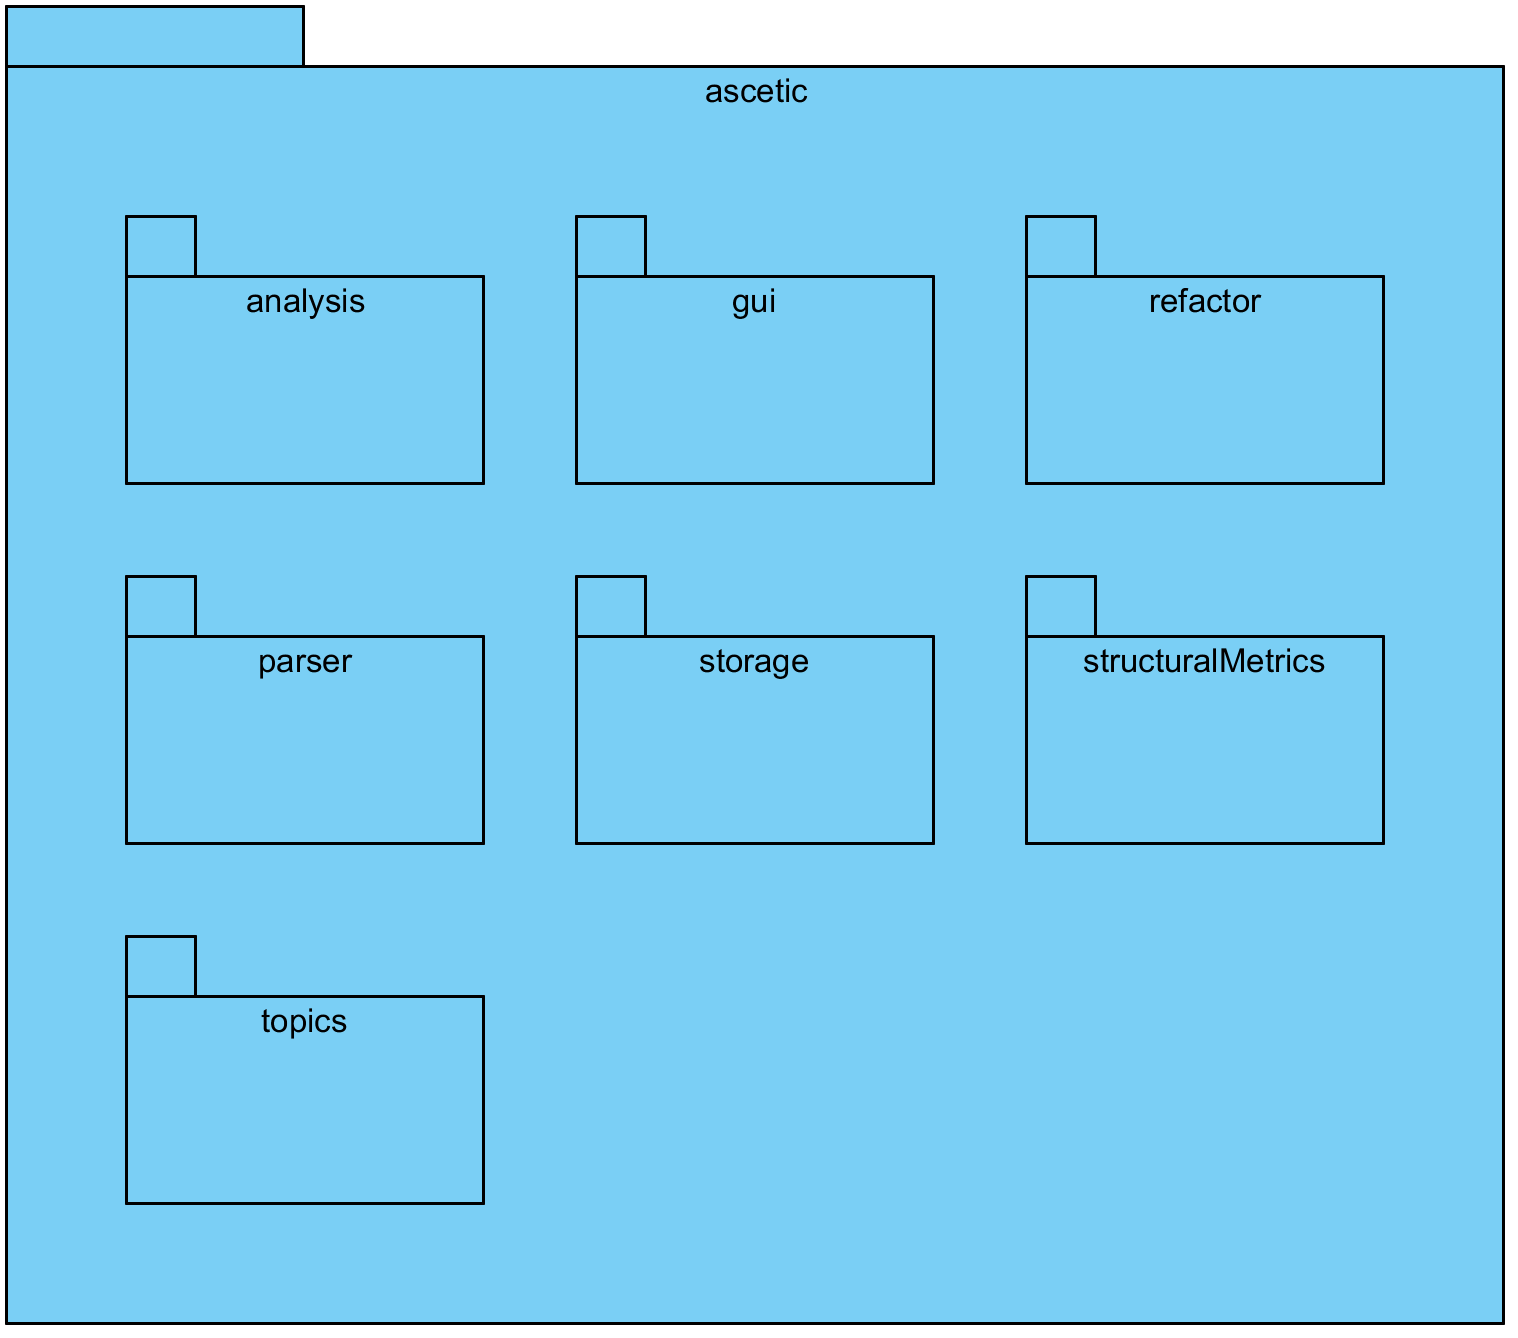
\includegraphics{diagrams/AsceticPackageDiagram}
			\end{figure}
			
			\subsubsection{Package analysis}
			Il sottopackage analysis si suddivide a sua volta in tre sottopackage, ossia: 
			\begin{figure}[!h]
				\centering
				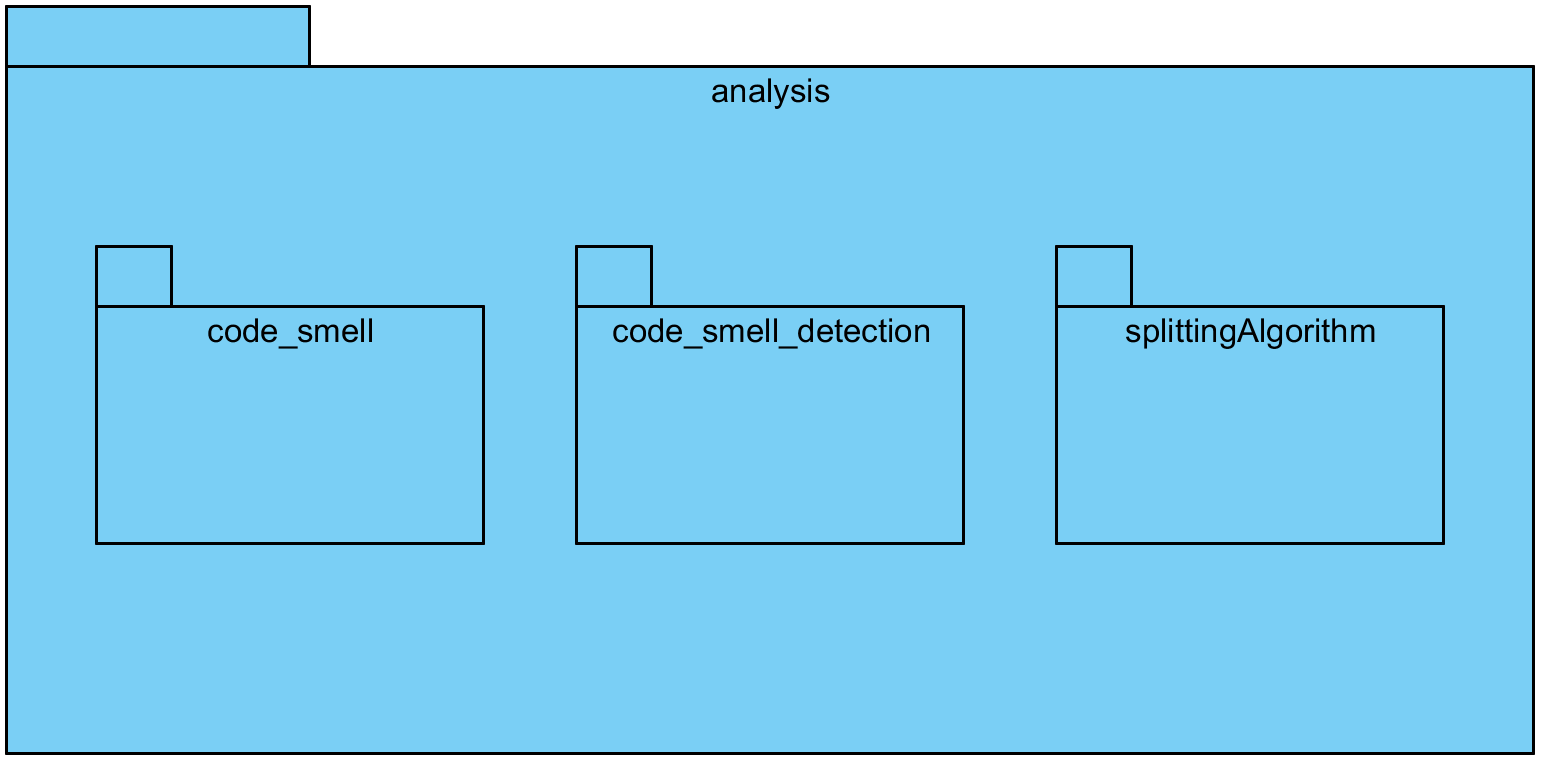
\includegraphics[width=12cm]{diagrams/AnalysisPackageDiagram}
			\end{figure}
						
			\begin{description}
				\item[2.1.1.1 Package code\_smell]
				\item \begin{figure}[!h]
					\centering
					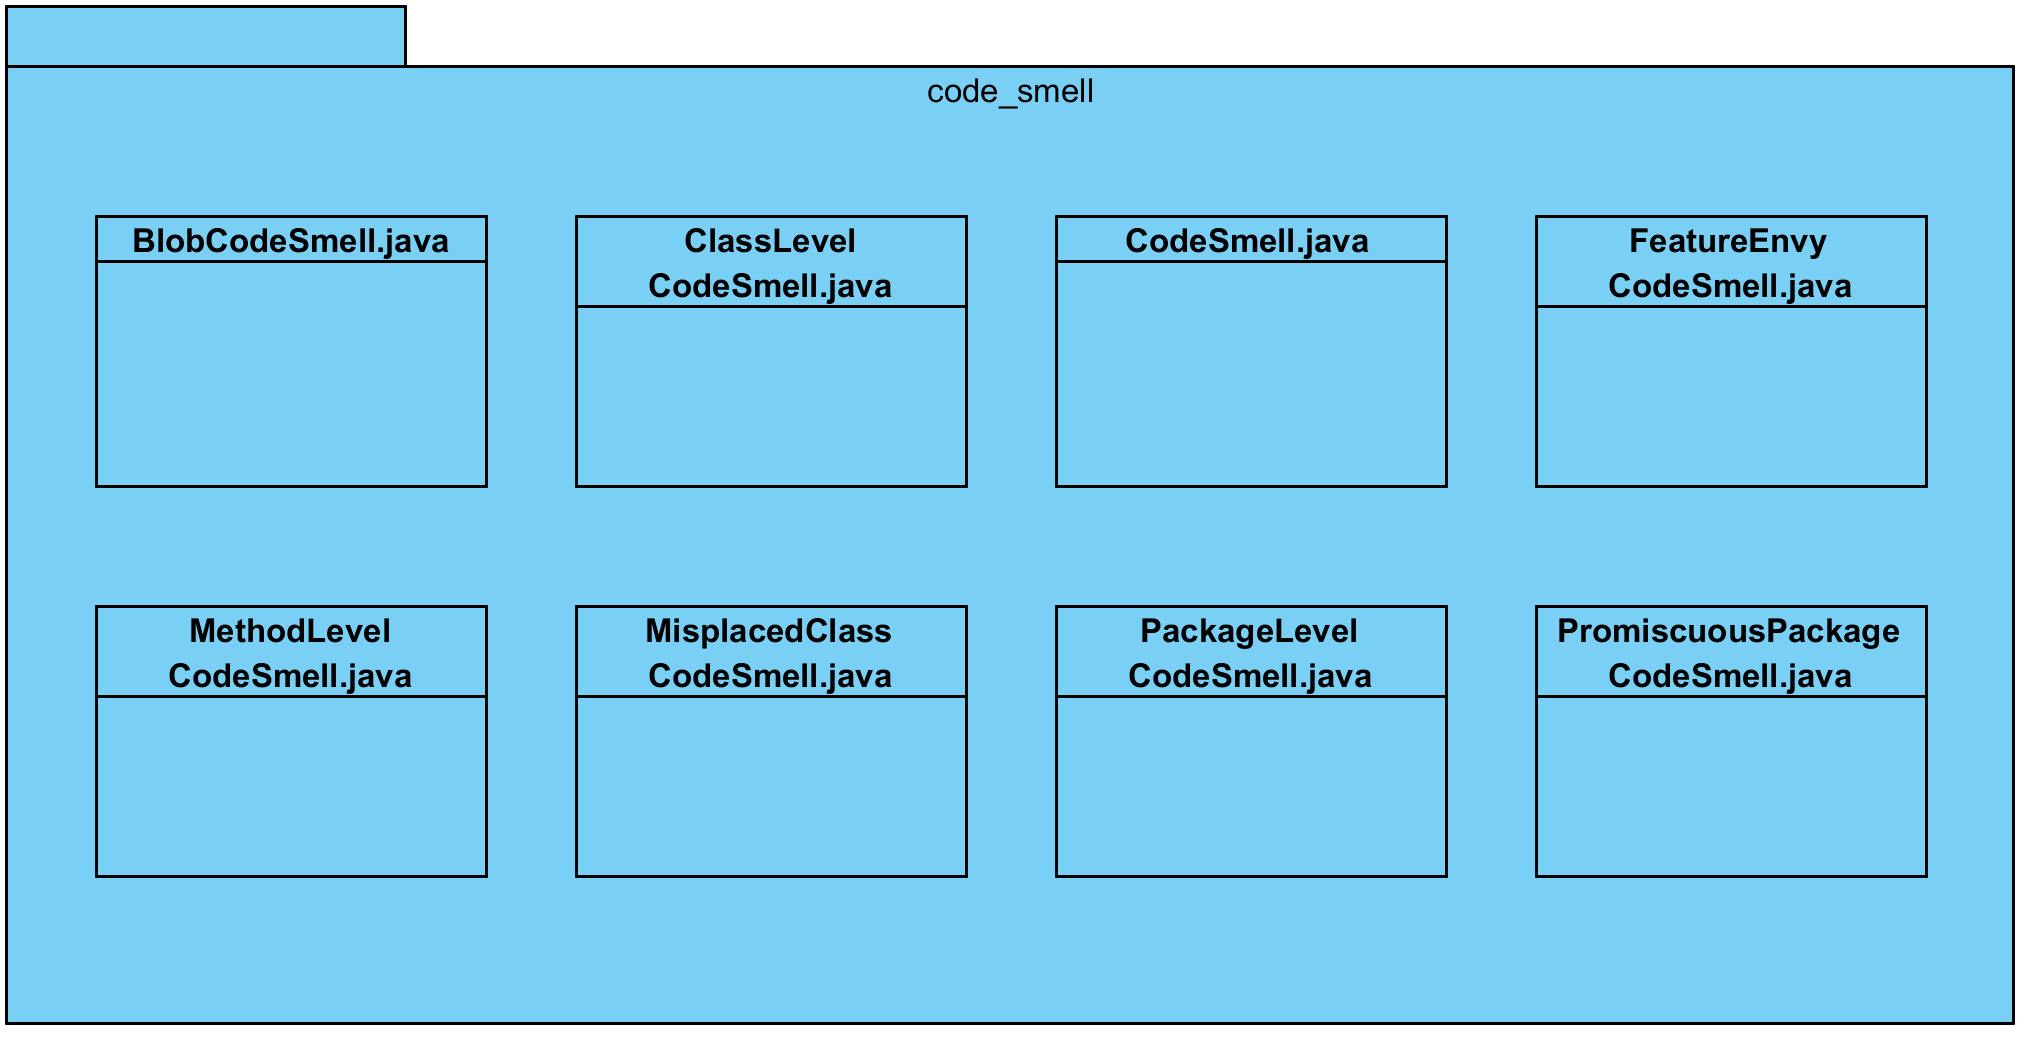
\includegraphics[width=13cm]{diagrams/Code_SmellPackageDiagram}
				\end{figure}
				Di seguito è riportata la tabella delle descrizioni di ogni classe appartenente al package code\_smell:
				\item \begin{tabular}{|p{7,6cm}|p{7,5cm}|}
					\hline
					\textbf{Classe} & \textbf{Descrizione}\\
					\hline
					BlobCodeSmell.java & Permette di istanziare il code smell Blob. \\
					\hline
					ClassLevelCodeSmell.java & Permette di istanziare tutti gli oggetti di tipo CodeSmell che riguardano l'ambito delle classi. \\
					\hline
					CodeSmell.java & Permette di tenere traccia nel database dei code smell individuati durante l'analisi del codice.\\
					\hline
					FeatureEnvyCodeSmell.java & Permette di istanziare il code smell Feature Envy.\\
					\hline
					MethodLevelCodeSmell.java & Permette di istanziare tutti gli oggetti di tipo CodeSmell che riguardano l'ambito dei metodi.\\
					\hline
					MisplacedClassCodeSmell.java & Permette di istanziare il code smell Misplaced Class. \\
					\hline
					PackageLevelCodeSmell.java & Permette di istanziare tutti gli oggetti di tipo CodeSmell che riguardano l'ambito dei package.\\
					\hline
					PromiscuousPackageCodeSmell.java & Permette di istanziare il code smell Promiscuous Package.\\
					\hline
				\end{tabular}
			\\\\
				\item[2.1.1.2 Package code\_smell\_detection] 
				\item Il sottopackage code\_smell\_detection si suddivide a sua volta in altri nove sottopackage, ossia:
				\item 	\begin{figure}[!h]
					\centering
					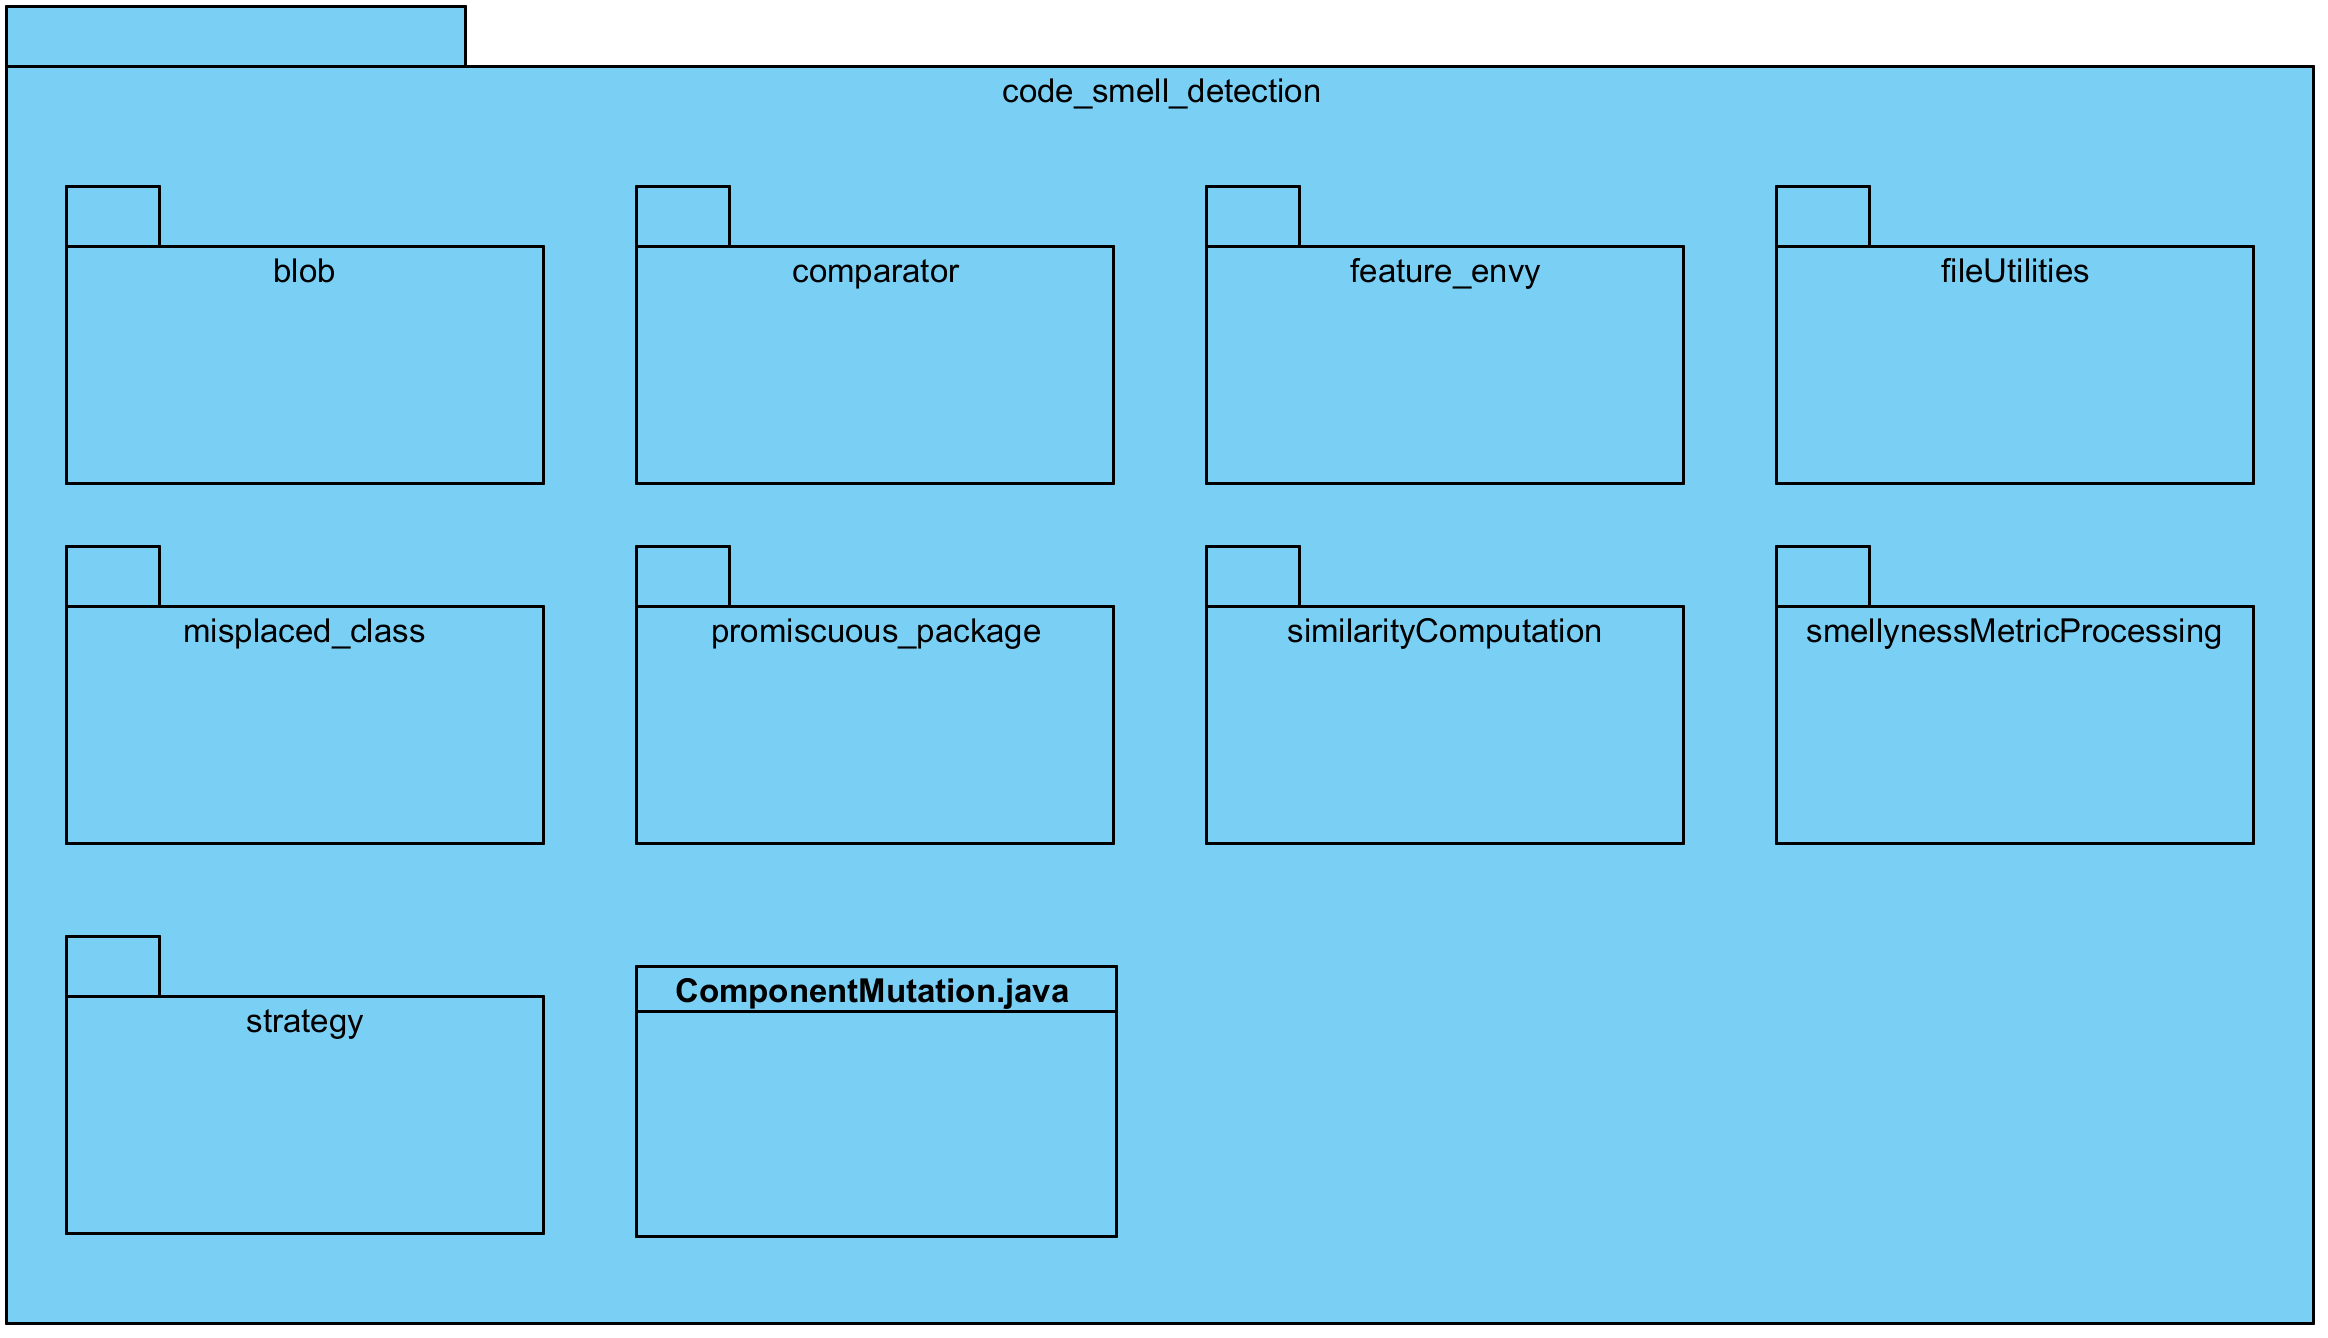
\includegraphics[width=16cm]{diagrams/Code_Smell_DetectionPackageDiagram}
				\end{figure}
				Di seguito è riportata la tabella della descrizione della classe appartenente al package\\code\_smell\_detection:
				\item \begin{tabular}{|p{7,6cm}|p{7,5cm}|}
					\hline
					\textbf{Classe} & \textbf{Descrizione}\\
					\hline
					ComponentMutation.java & Permette di convertire un qualsiasi Bean in String, semplicemente inserendo il contenuto testuale completo del Bean in una stringa.\\
					\hline
				\end{tabular}
				\newpage
				\item[ 2.1.1.2.1 Package blob]
				\item \begin{figure}[!h]
					\centering
					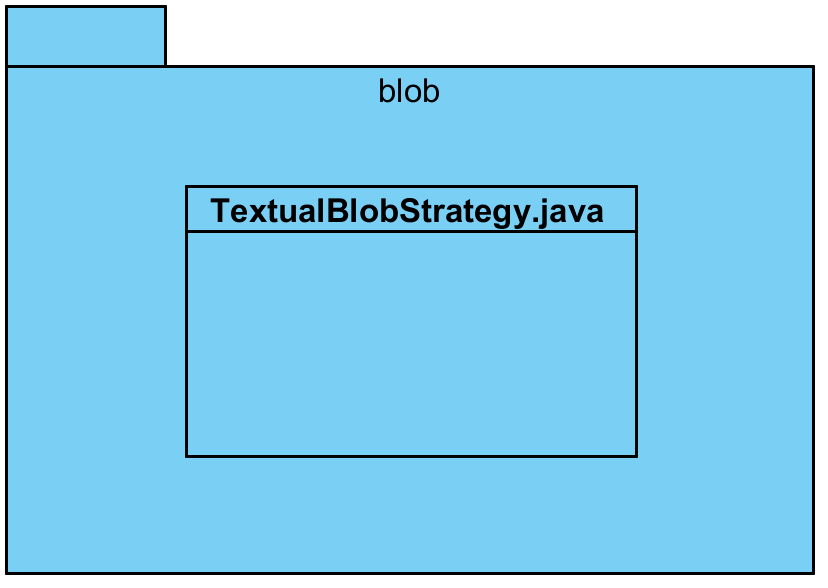
\includegraphics{diagrams/BlobPackageDiagram}
				\end{figure}
			Di seguito è riportata la tabella della descrizione della classe appartenente al package blob:	
				\item \begin{tabular}{|p{7,6cm}|p{7,5cm}|}
					\hline
					\textbf{Classe} & \textbf{Descrizione}\\
					\hline
					TextualBlobStrategy.java & Permette di rilevare attraverso il contenuto testuale, implementando lo Strategy adeguato, i code smell di tipo Blob. \\
					\hline
				\end{tabular}					
				\item[ 2.1.1.2.2 Package comparator] 
				\item \begin{figure}[!h]
					\centering
					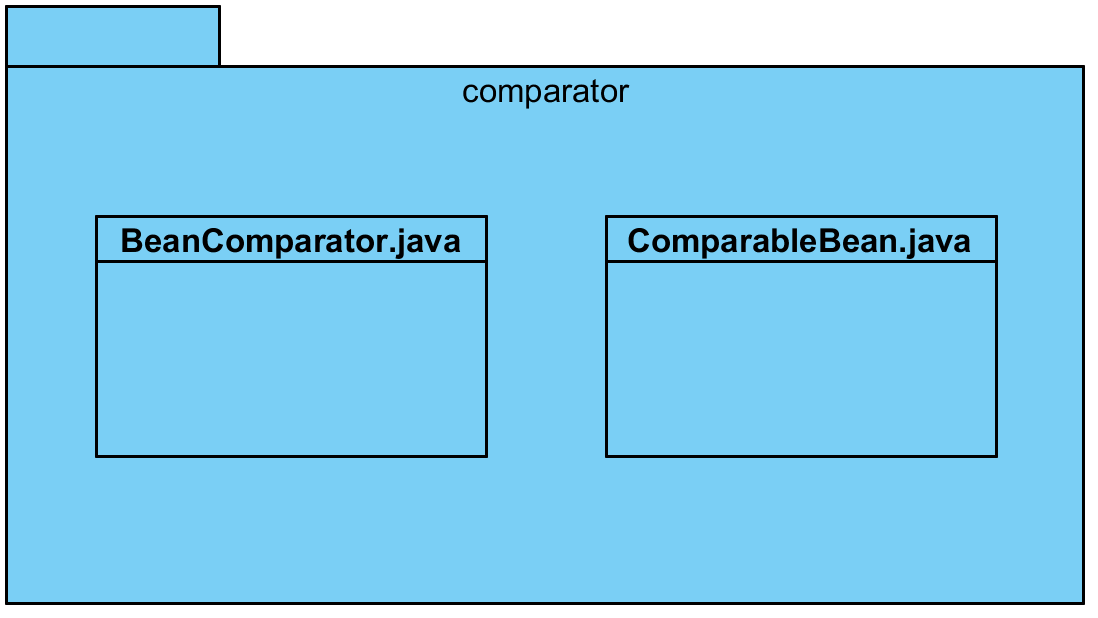
\includegraphics{diagrams/ComparatorPackageDiagram}
				\end{figure}
				Di seguito sono riportate le tabelle delle descrizioni della classe e dell'interfaccia appartenenti al package comparator:
				\item \begin{tabular}{|p{7,6cm}|p{7,5cm}|}
					\hline
					\textbf{Classe} & \textbf{Descrizione}\\
					\hline
					BeanComparator.java & Permette di comparare due Bean. \\
					\hline
				\end{tabular}
				\item \begin{tabular}{|p{7,6cm}|p{7,5cm}|}
					\hline
					\textbf{Interfaccia} & \textbf{Descrizione}\\
					\hline
					ComparableBean.java & Dichiara il metodo che permette di trovare uguaglianze fra i Bean. \\
					\hline
				\end{tabular}
				
				\item[ 2.1.1.2.3 Package feature\_envy] 
				\item \begin{figure}[!h]
					\centering
					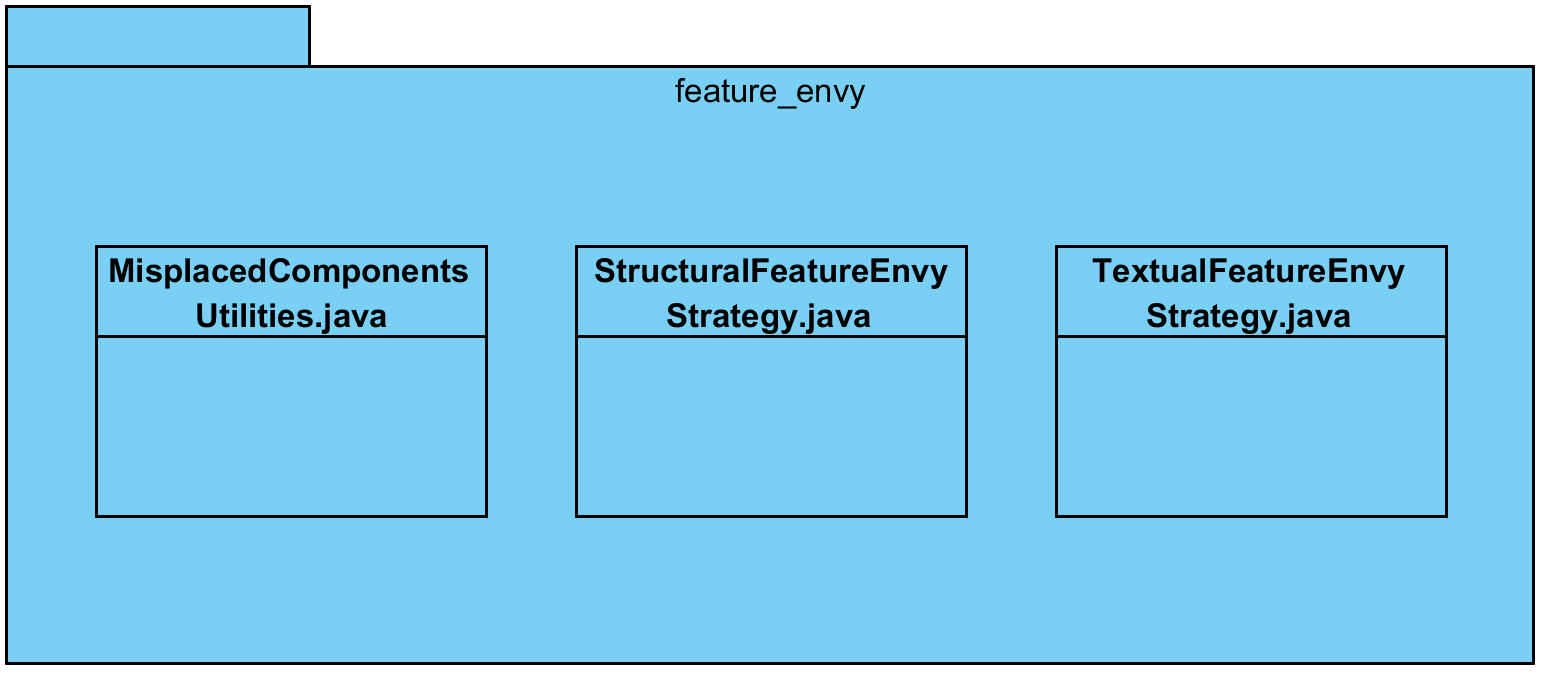
\includegraphics{diagrams/Feature_EnvyPackageDiagram}
				\end{figure}
				Di seguito è riportata la tabella delle descrizioni delle classi appartenenti al package feature\_envy:
				\item \begin{tabular}{|p{7,6cm}|p{7,5cm}|}
					\hline
					\textbf{Classe} & \textbf{Descrizione}\\
					\hline
					MisplacedComponentsUtilities.java & Permette di identificare le possibili classi affette da code smell di tipo Feature Envy in base al calcolo del coseno. \\
					\hline
					StructuralFeatureEnvyStrategy.java & Permette di identificare, a livello strutturale, i code smell di tipo Feature Envy. \\
					\hline
					TextualFeatureEnvyStrategy.java & Permette di rilevare attraverso il contenuto testuale i code smell di tipo Feature Envy. \\
					\hline
				\end{tabular}
				
				\item[ 2.1.1.2.4 Package fileUtilities] 
				\item \begin{figure}[!h]
					\centering					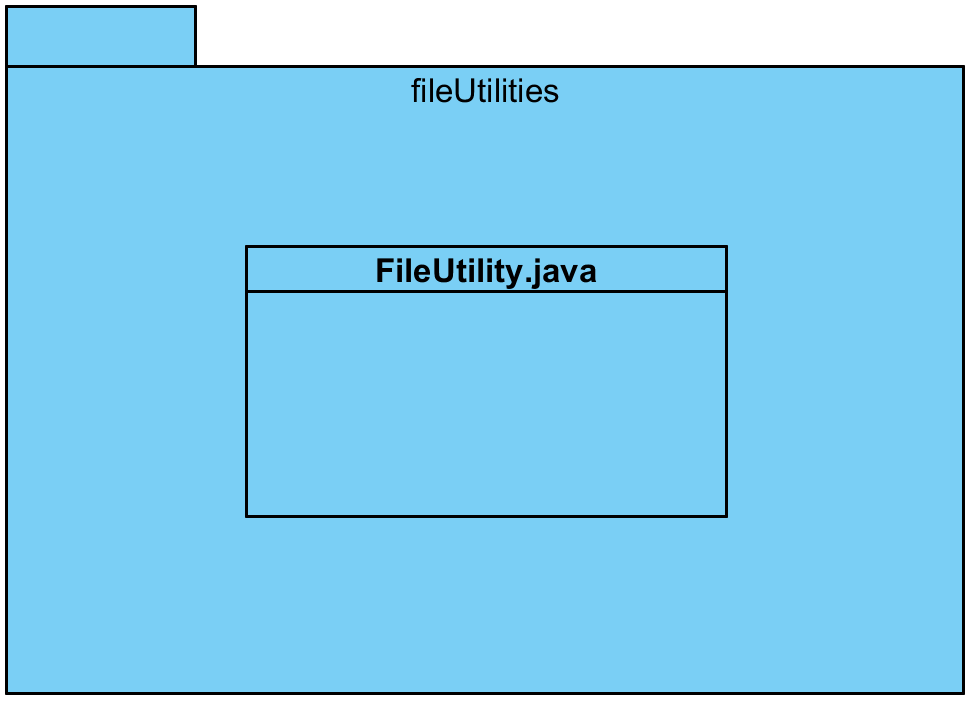
\includegraphics{diagrams/FileUtilityPackageDiagram}
				\end{figure}
				Di seguito è riportata la tabella della descrizione della classe appartenente al package fileUtilities:
				\item \begin{tabular}{|p{7,6cm}|p{7,5cm}|}
					\hline
					\textbf{Classe} & \textbf{Descrizione}\\
					\hline
					FileUtility.java & Permette di effettuare operazioni su file. \\
					\hline
				\end{tabular}
				
				\item[ 2.1.1.2.5 Package misplaced\_class] \item \begin{figure}[!h]
					\centering
					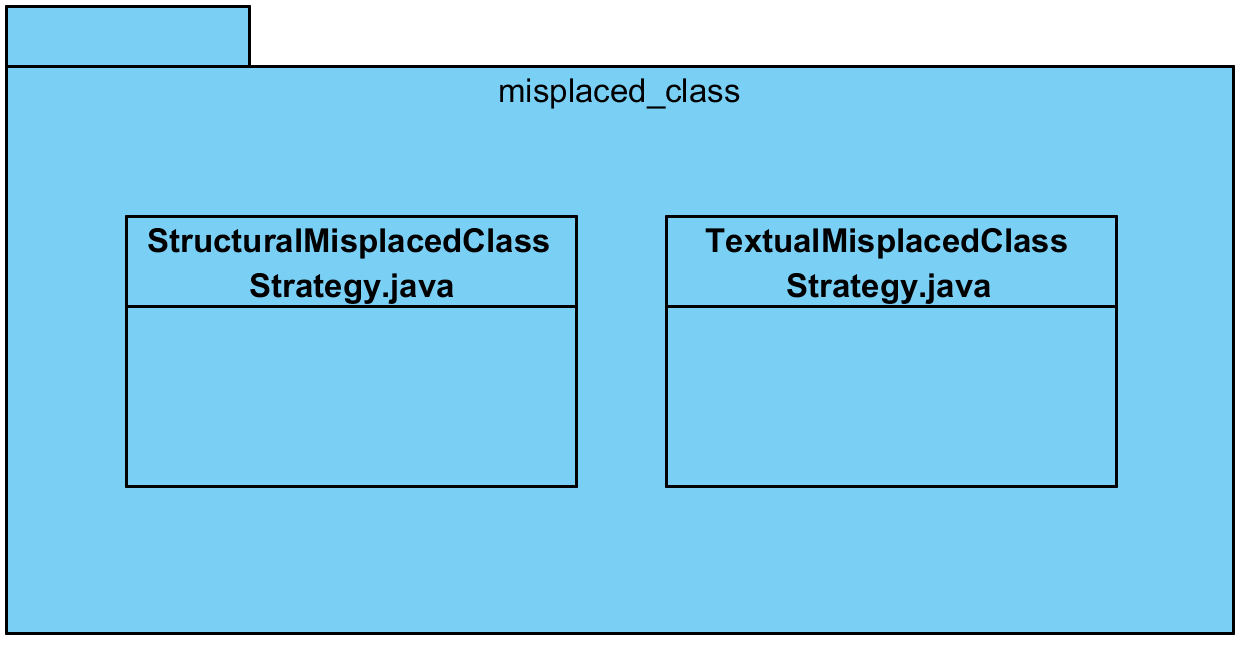
\includegraphics{diagrams/Misplaced_ClassPackageDiagram}
				\end{figure}
				Di seguito è riportata la tabella delle descrizioni delle classi appartenenti al package \\misplaced\_class:
				\item \begin{tabular}{|p{7,6cm}|p{7,5cm}|}
					\hline
					\textbf{Classe} & \textbf{Descrizione}\\
					\hline
					StructuralMisplacedClassStrategy.java & Permette di identificare, a livello strutturale, i code smell di tipo Misplaced Class. \\
					\hline
					TextualMisplacedClassStrategy.java & Permette di rilevare  attraverso il contenuto testuale i code smell di tipo Misplaced Class. \\
					\hline
				\end{tabular}
				\newpage	
				\item[ 2.1.1.2.6 Package promiscuous\_package] \item \begin{figure}[!h]
					\centering
					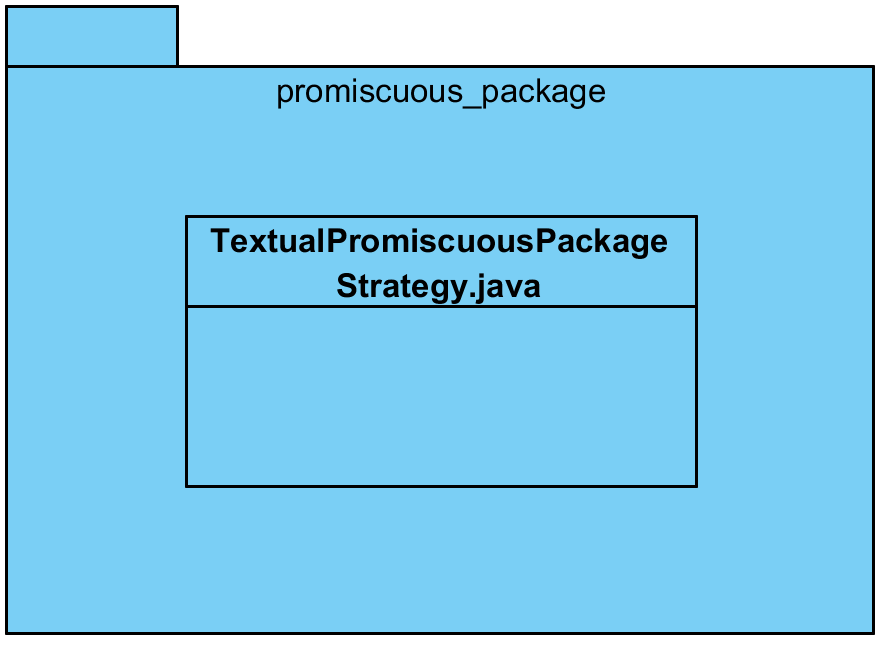
\includegraphics{diagrams/Promiscuous_PackagePackageDiagram}
				\end{figure}
				Di seguito è riportata la tabella della descrizione della classe appartenente al package \\promiscuous\_package:
				\item \begin{tabular}{|p{7,6cm}|p{7,5cm}|}
					\hline
					\textbf{Classe} & \textbf{Descrizione}\\
					\hline
					TextualPromiscuousPackageStrategy.java & Permette di rilevare attraverso il contenuto testuale i code smell di tipo Promiscuous Package. \\
					\hline
				\end{tabular}
					
				\item[ 2.1.1.2.7 Package similarityComputation] \item \begin{figure}[!h]
					\centering
					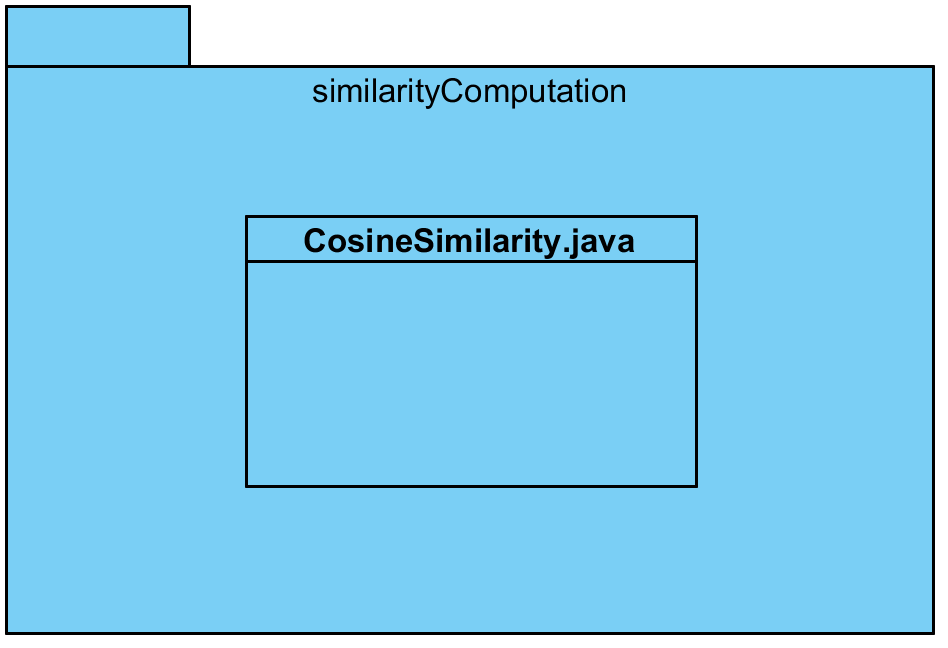
\includegraphics{diagrams/SimilarityComputationPackageDiagram}
				\end{figure}
			Di seguito è riportata la tabella della descrizione della classe appartenente al package \\similarityComputation:
				\item \begin{tabular}{|p{7,6cm}|p{7,5cm}|}
					\hline
					\textbf{Classe} & \textbf{Descrizione}\\
					\hline
					CosineSimilarity.java & Permette di calcolare la differenza fra due Bean attraverso il calcolo del coseno per verificare la presenza di un code smell. \\
					\hline
				\end{tabular}
		
				\item[ 2.1.1.2.8 Package smellynessMetricProcessing]
				\item \begin{figure}[!h]
					\centering
					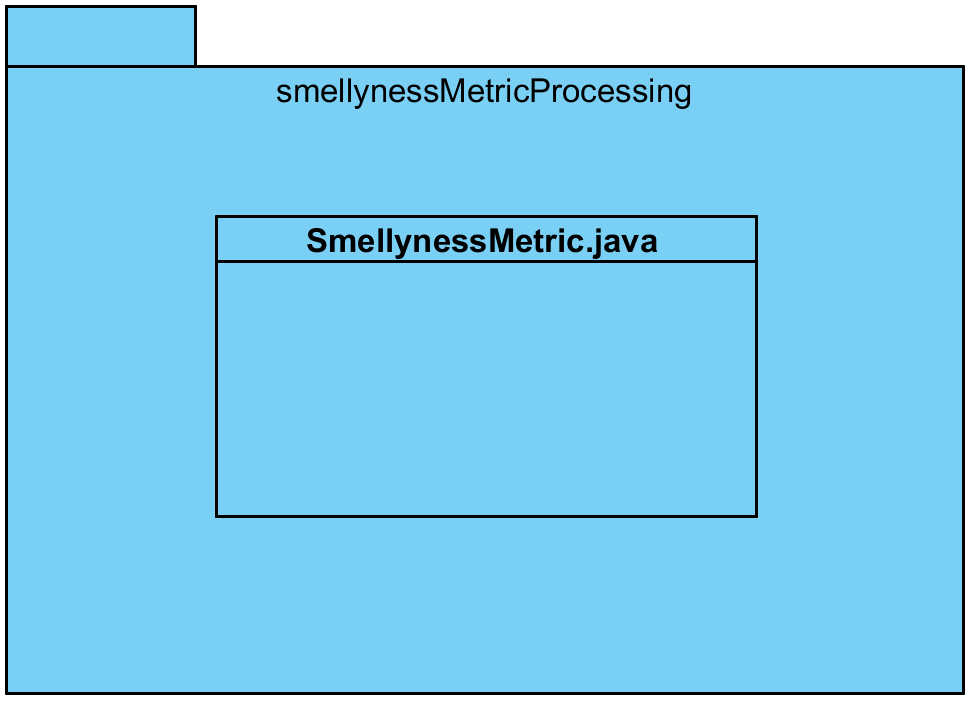
\includegraphics{diagrams/SmellynessMetricProcessingPackageDiagram}
				\end{figure}
				Di seguito è riportata la tabella della descrizione della classe appartenente al package \\smellynessMetricProcessing:
				\item \begin{tabular}{|p{7,6cm}|p{7,5cm}|}
					\hline
					\textbf{Classe} & \textbf{Descrizione}\\
					\hline
					SmellynessMetric.java & Permette di calcolare le metriche all'interno del testo di un Bean. \\
					\hline
				\end{tabular}
					
				\item[ 2.1.1.2.9 Package strategy] 
				\item \begin{figure}[!h]
					\centering
					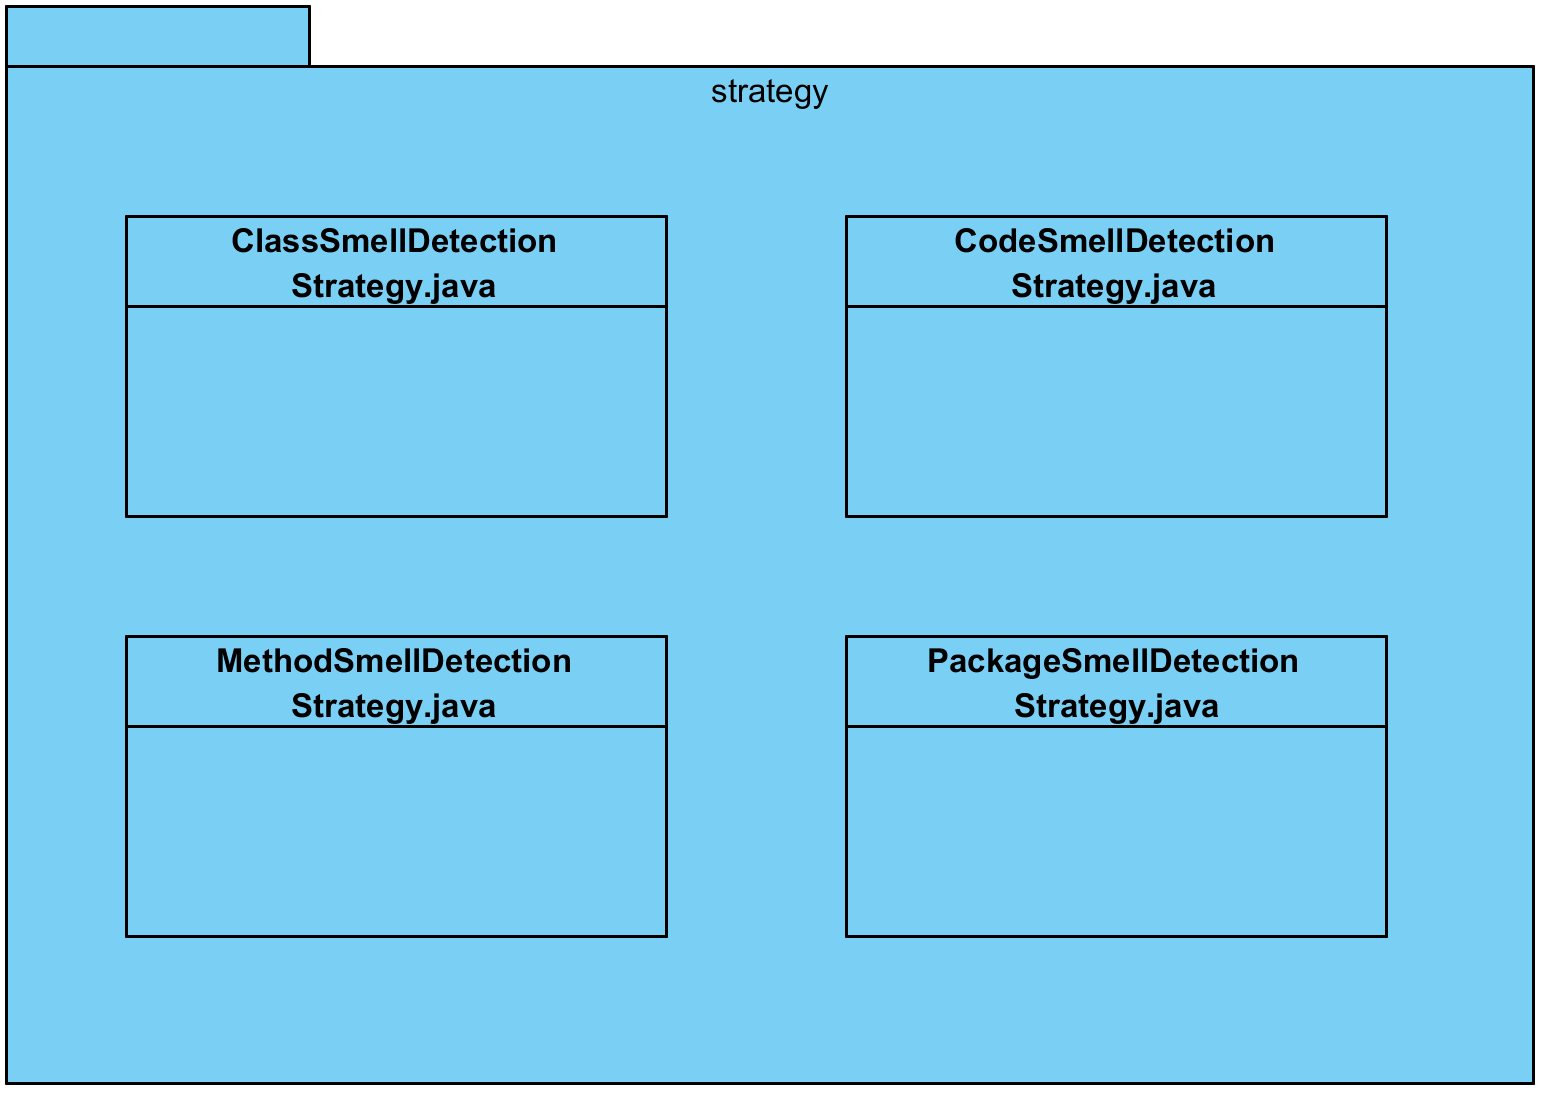
\includegraphics{diagrams/StrategyAnalysisPackageDiagram}
				\end{figure}
				Di seguito è riportata la tabella delle descrizioni delle interfacce appartenenti al package strategy:
				\item \begin{tabular}{|p{7,6cm}|p{7,5cm}|}
					\hline
					\textbf{Interfaccia} & \textbf{Descrizione}\\
					\hline
					ClassSmellDetectionStrategy.java & Dichiara i metodi da implementare negli Strategy addetti al rilevamento
					di code smell nelle classi. \\
					\hline
					CodeSmellDetectionStrategy.java & Dichiara i metodi da implementare negli Strategy. \\
					\hline
					MethodSmellDetectionStrategy.java & Dichiara i metodi da implementare negli Strategy addetti al rilevamento
					di code smell nei metodi. \\
					\hline
					PackageSmellDetectionStrategy.java & Dichiara i metodi da implementare negli Strategy addetti al rilevamento
					di code smell nei package. \\
					\hline
				\end{tabular}
			
			
			\item[2.1.1.3 Package splittingAlgorithm] 
			\item Il sottopackage splittingAlgorithm si suddivide a sua volta in un altro sottopackage, ossia:
			\item 	\begin{figure}[!h]
				\centering
				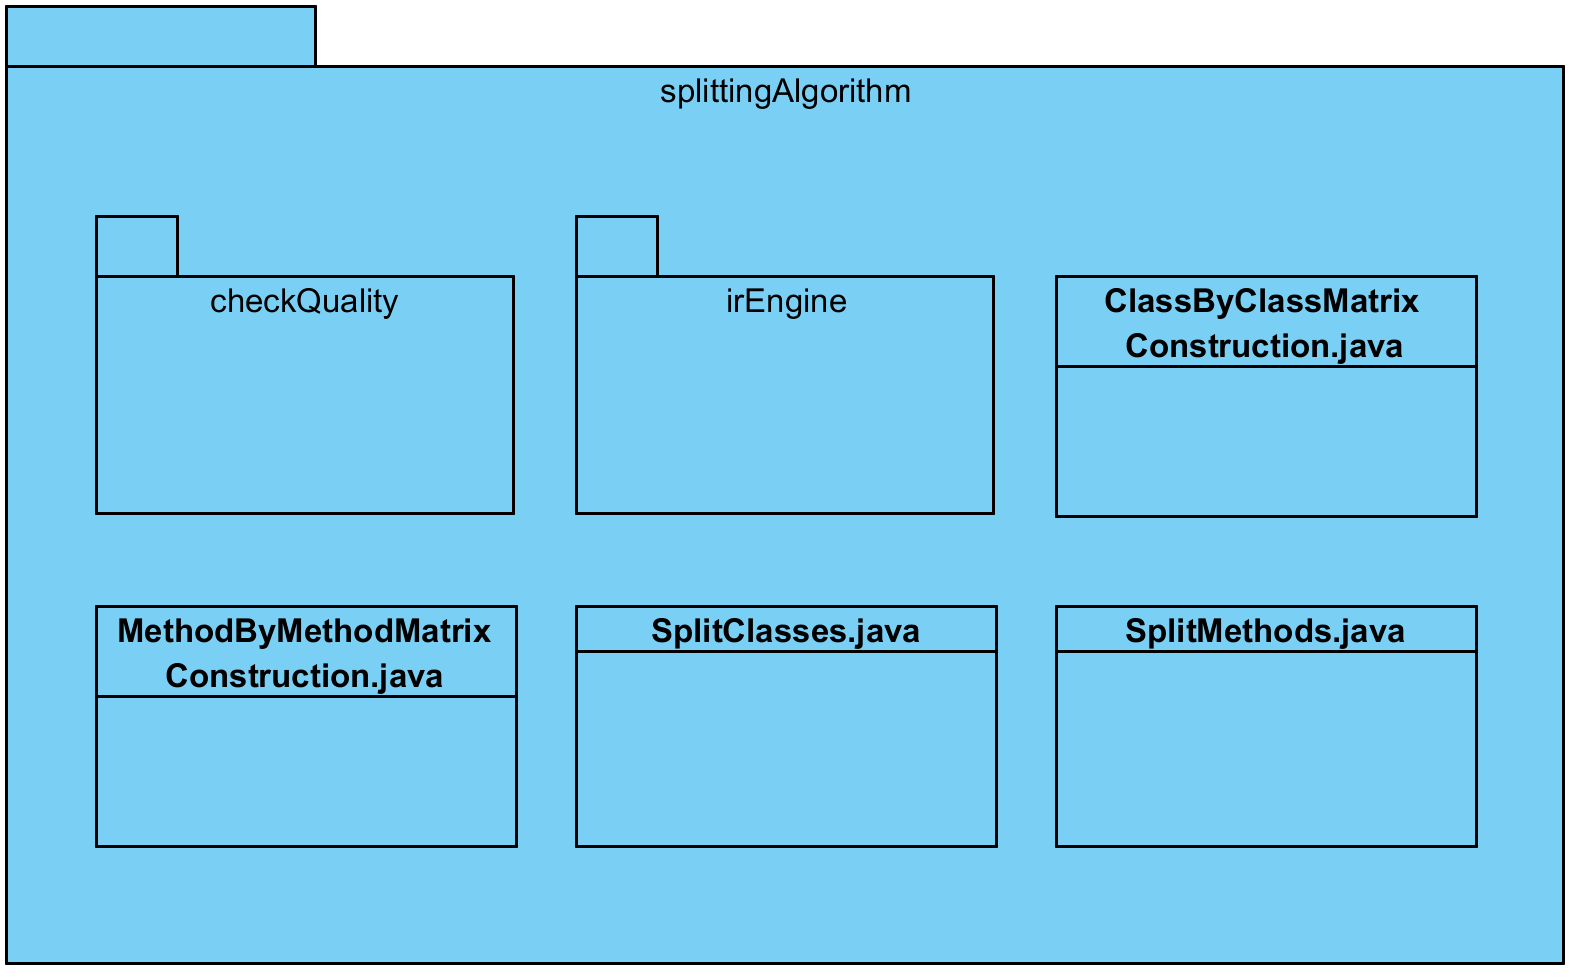
\includegraphics{diagrams/SplittingAlgorithmPackageDiagram}
			\end{figure}
			Di seguito è riportata la tabella delle descrizioni delle classi appartenenti al package splittingAlgorithm:
			\item \begin{tabular}{|p{7,6cm}|p{7,5cm}|}
				\hline
				\textbf{Classe} & \textbf{Descrizione}\\
				\hline
				ClassByClassMatrixConstruction.java & Permette di creare una matrice classe per classe.\\
				\hline
				MethodByMethodMatrixConstruction.java & Permette di creare una matrice metodo per metodo. \\
				\hline
				SplitClasses.java & Permette di dividere una classe in più classi.\\
				\hline
				SplitMethods.java & Permette di dividere un metodo in più metodi.\\
				\hline
			\end{tabular}
		\item[ 2.1.1.3.1 Package packageLevel] 
		\item Il sottopackage packageLevel è contenuto nel package checkQuality:
		\item \begin{figure}[!h]
			\centering
			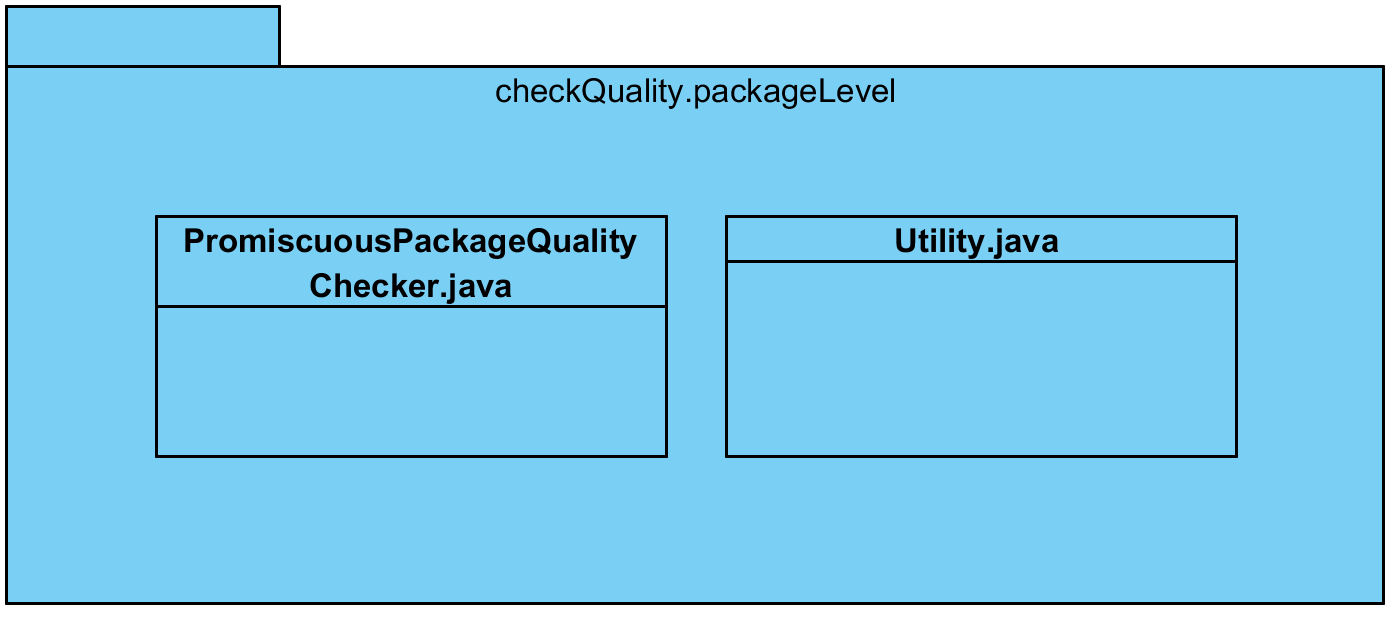
\includegraphics{diagrams/CheckQualityPackageLevelPackageDiagram}
		\end{figure}
		Di seguito è riportata la tabella delle descrizioni delle classi appartenenti al package packageLevel:
		\item \begin{tabular}{|p{7,6cm}|p{7,5cm}|}
			\hline
			\textbf{Classe} & \textbf{Descrizione}\\
			\hline
			PromiscuousPackageQualityChecker.java & Permette di calcolare delle metriche su package per controllarne la qualità. \\
			\hline
			Utility.java & Permette di effettuare operazioni su file. \\
			\hline
		\end{tabular}	
	\item[ 2.1.1.3.2 Package irEngine] 
	\item \begin{figure}[!h]
		\centering
		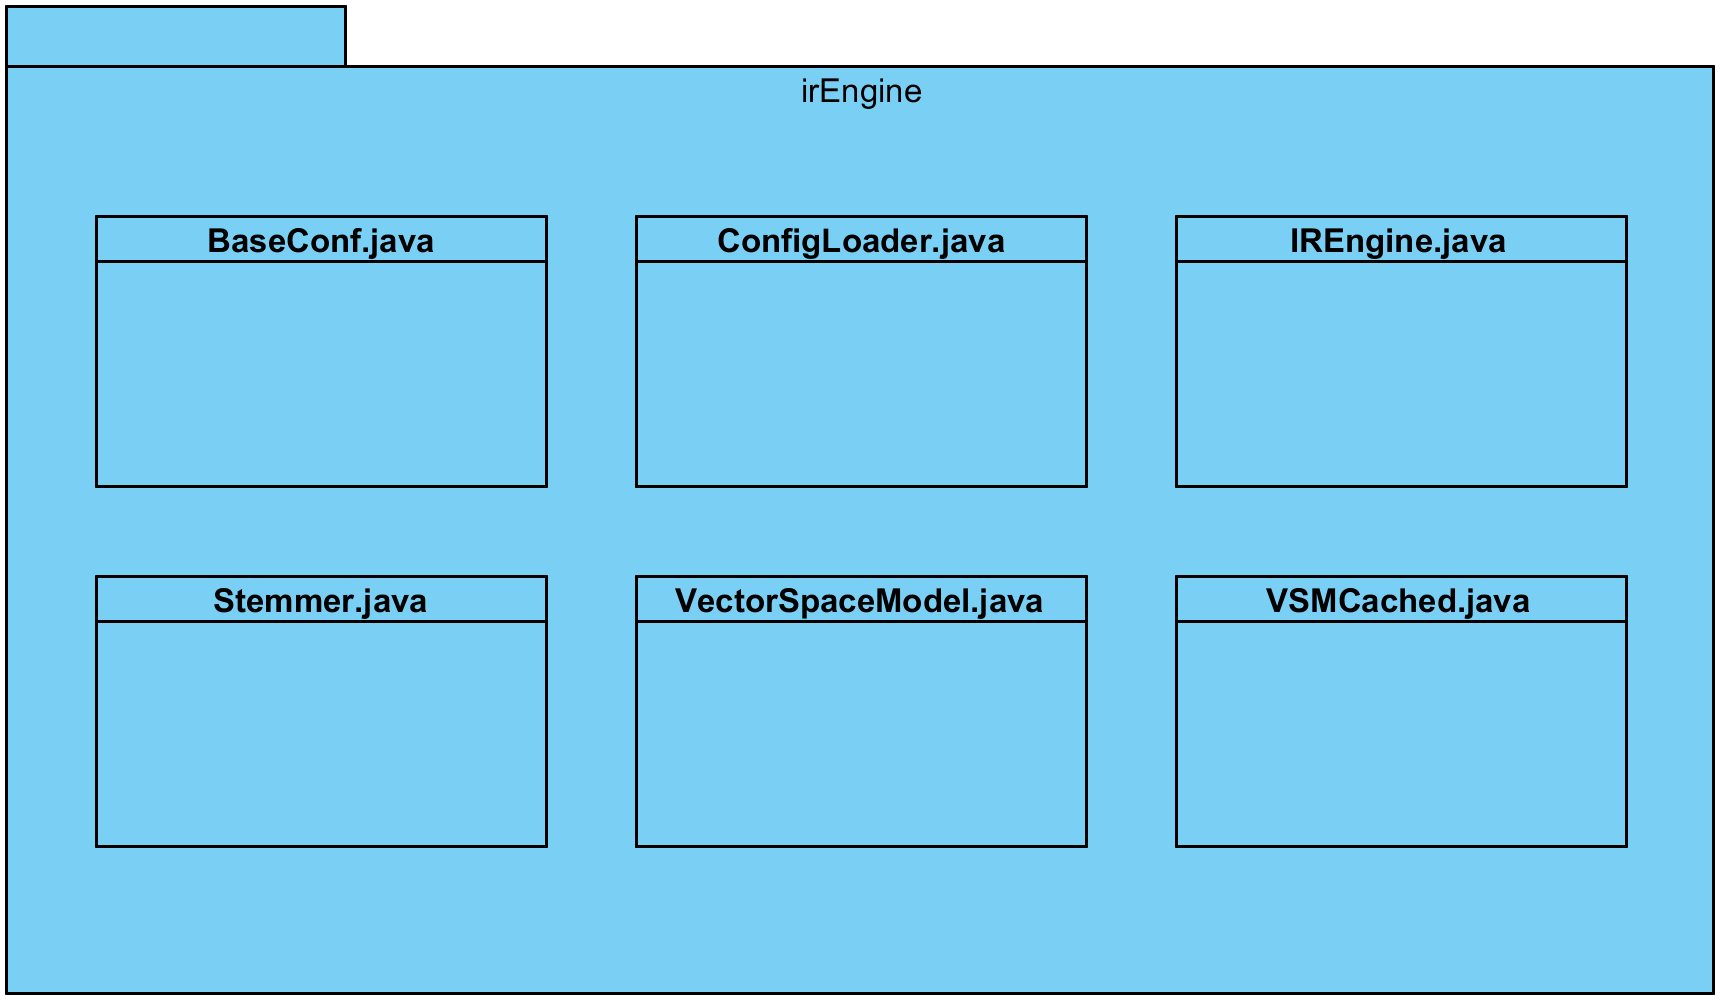
\includegraphics{diagrams/IREnginePackageDiagram}
	\end{figure}
	Di seguito è riportata la tabella delle descrizioni delle classi e dell'interfaccia appartenenti al package irEngine:
	\item \begin{tabular}{|p{7,6cm}|p{7,5cm}|}
		\hline
		\textbf{Classe} & \textbf{Descrizione}\\
		\hline
		BaseConf.java & Permette di creare la configurazione standard del plug-in. \\
		\hline
		ConfigLoader.java & Permette di caricare il file della configurazione standard del plug-in. \\
		\hline
		Stemmer.java & Permette di ridurre termini derivati alle parole da cui derivano.  \\
		\hline
		VectorSpaceModel.java & Permette di effettuare operazioni di conteggio e di estrazione dei termini dai documenti contenenti matrici di termini e di generare quest'ultime. \\
		\hline
		VSMCached.java & Permette di, estendendo VectorSpaceModel, effettuare operazioni sull'istanza dell'oggetto matrice.  \\
		\hline
	\end{tabular}
	\item \begin{tabular}{|p{7,6cm}|p{7,5cm}|}
		\hline
		\textbf{Interfaccia} & \textbf{Descrizione}\\
		\hline
		IREngine.java & Dichiara i metodi per la creazione di documenti contenente matrici di termini e per il calcolo delle somiglianze fra documenti. \\
		\hline
	\end{tabular}	
			\end{description}
		\subsubsection{Package gui}
			Il package gui contiene i seguenti sottopackage:
			 \begin{figure}[!h]
				\centering
				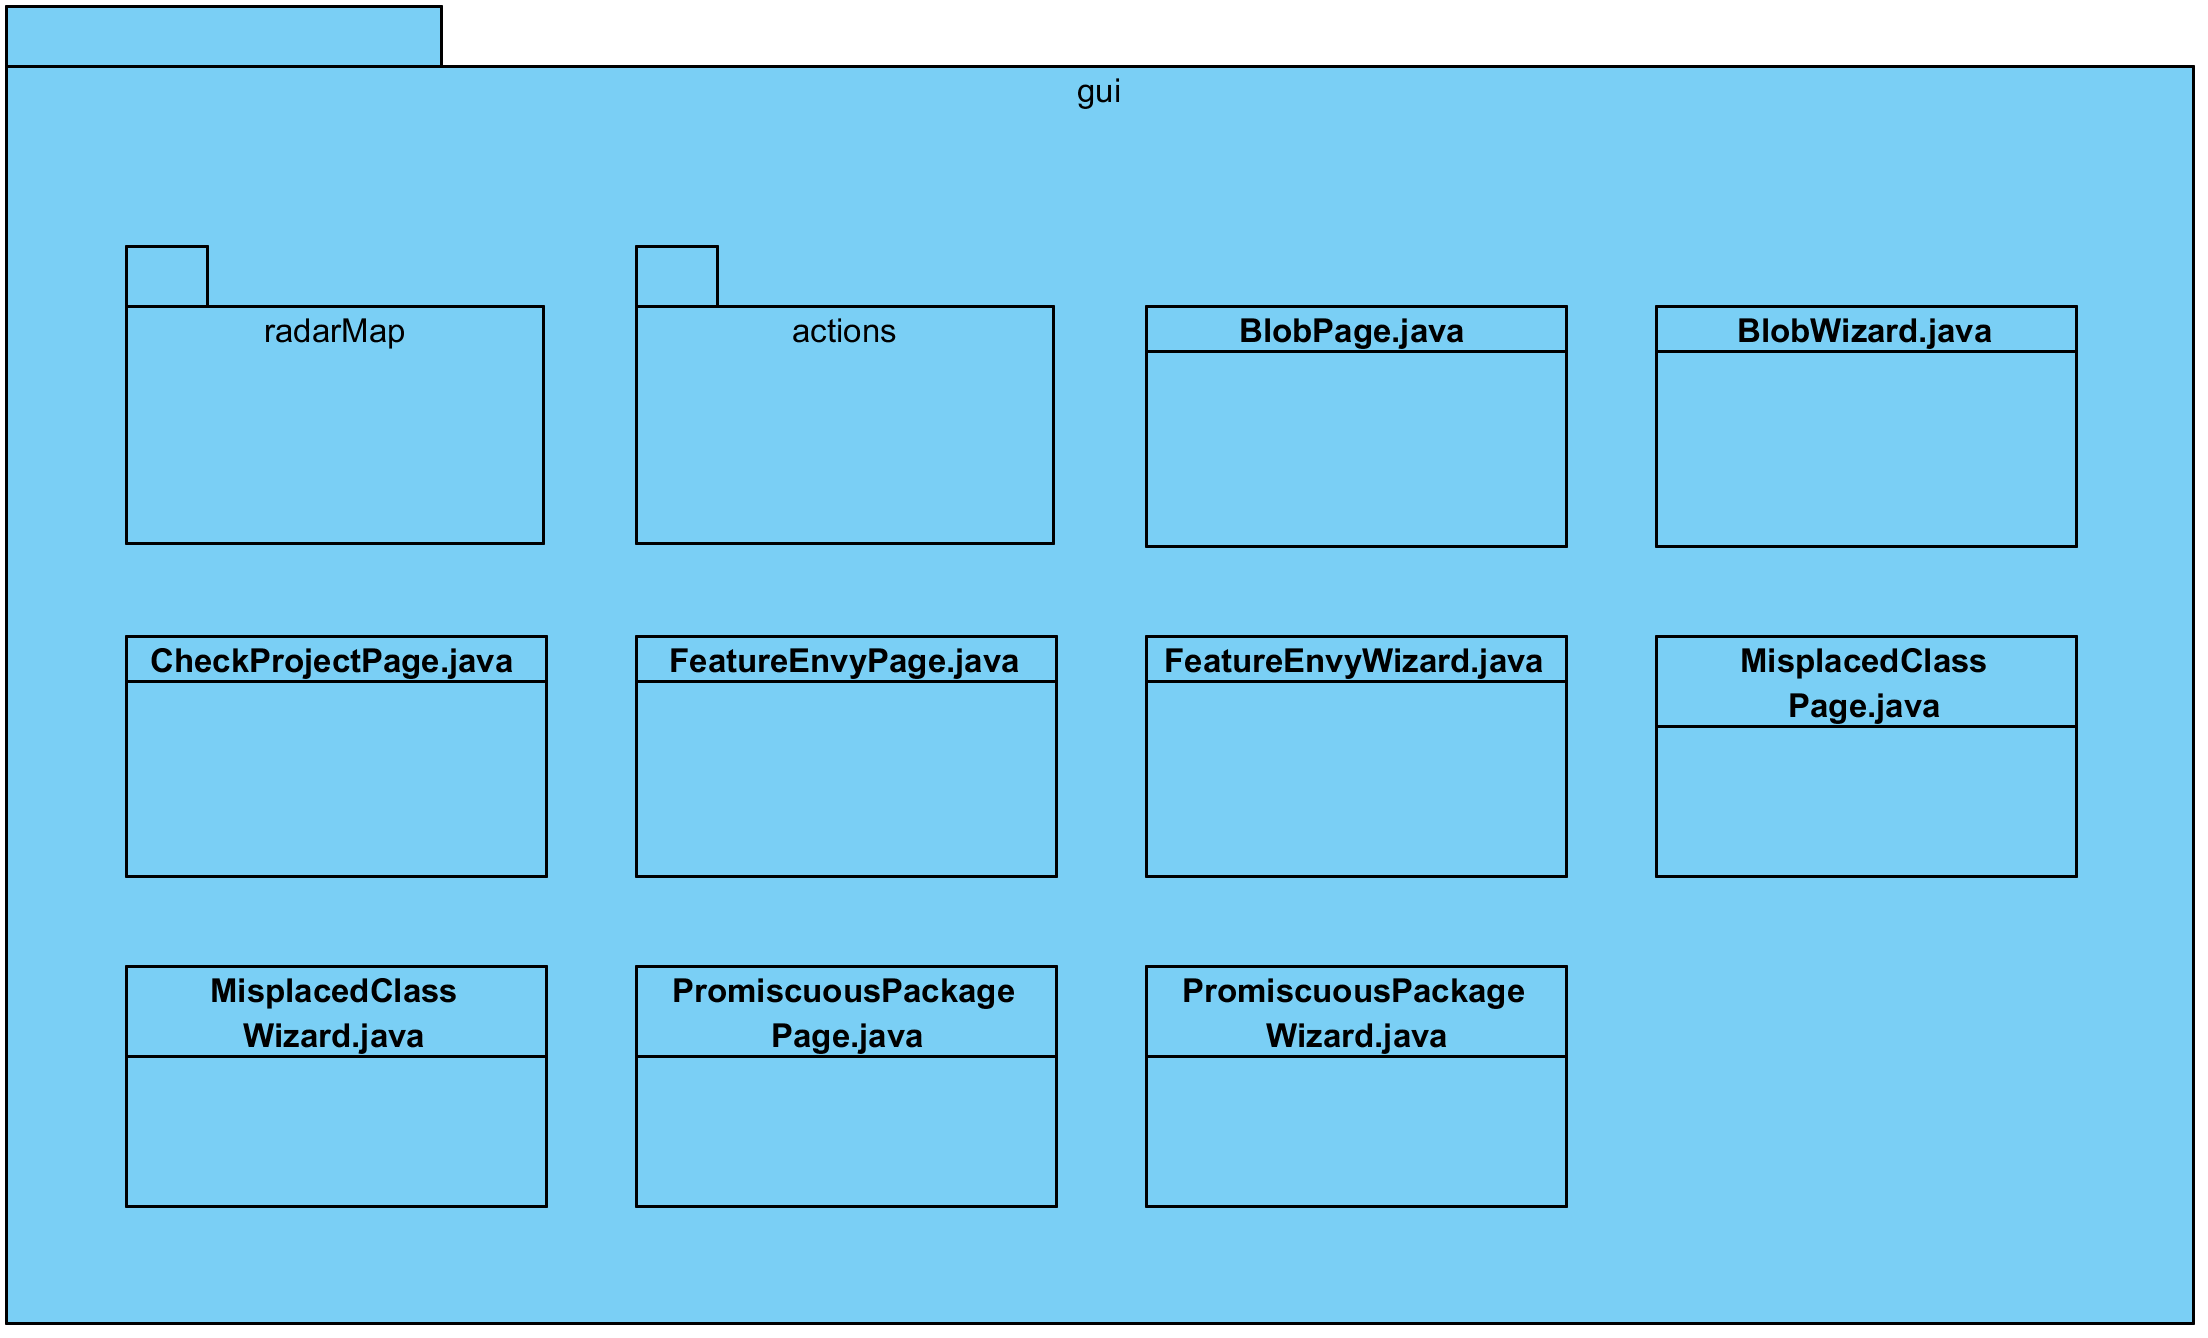
\includegraphics[width=15cm]{diagrams/GUIPackageDiagram}
			\end{figure}
		\begin{description}
			\item Di seguito è riportata la tabella delle descrizioni delle classi appartenenti al package gui:
			\item \begin{tabular}{|p{7,6cm}|p{7,5cm}|}
				\hline
				\textbf{Classe} & \textbf{Descrizione}\\
				\hline
				BlobPage.java & Permette di visualizzare la pagina di analisi dell'elemento affetto da code smell Blob.  \\
				\hline
				BlobWizard.java & Permette di visualizzare la pagina di refactoring dell'elemento affetto da code smell Blob.\\
				\hline
				CheckProjectPage.java & Permette di avviare la schermata principale del plug-in.\\
				\hline
				FeatureEnvyPage.java & Permette di visualizzare la pagina di analisi dell'elemento affetto da code smell Feature Envy. \\
				\hline
				FeatureEnvyWizard.java & Permette di visualizzare la pagina di refactoring dell'elemento affetto da code smell Feature Envy.\\
				\hline
				MisplacedClassPage.java & Permette di  visualizzare la pagina di analisi dell'elemento affetto da code smell Misplaced Class.\\
				\hline
				MisplacedClassWizard.java & Permette di visualizzare la pagina di refactoring dell'elemento affetto da code smell Misplaced Class.\\
				\hline
				PromiscuousPackagePage.java & Permette di  visualizzare la pagina di analisi dell'elemento affetto da code smell Promiscuous Package.\\
				\hline
				PromiscuousPackageWizard.java & Permette di visualizzare la pagina di refactoring dell'elemento affetto da code smell Promiscuous Package.\\
				\hline
			\end{tabular}

			\item[ 2.1.2.1 Package radarMap] 
		\item \begin{figure}[!h]
			\centering
			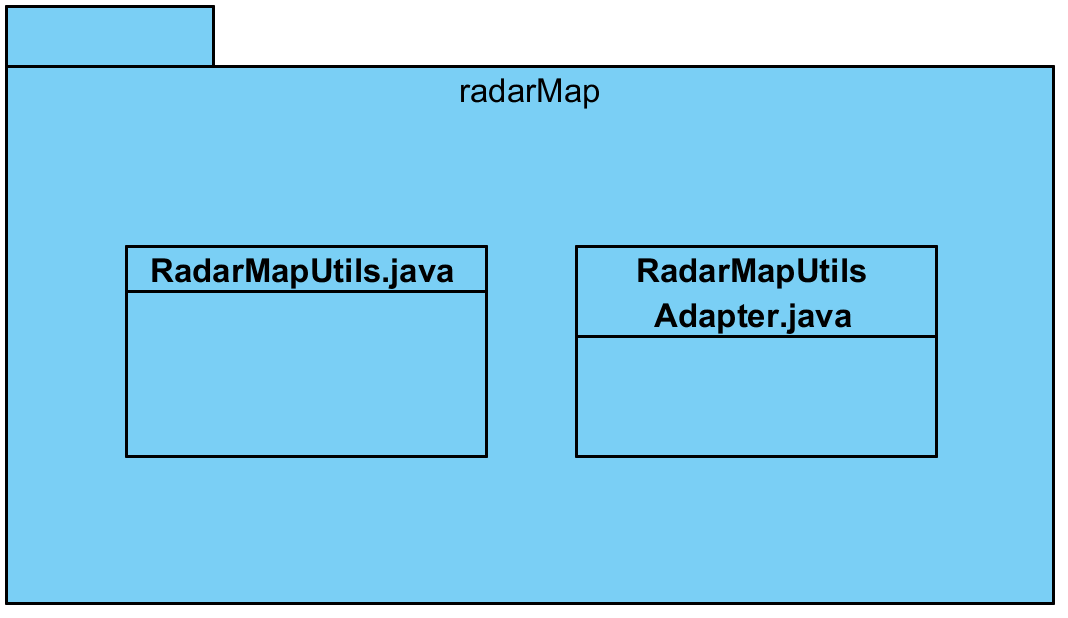
\includegraphics{diagrams/RadarMapPackageDiagram}
		\end{figure}
		Di seguito è riportata la tabella delle descrizioni della classe e dell'interfaccia appartenenti al package radarMap:
		\item \begin{tabular}{|p{7,6cm}|p{7,5cm}|}
			\hline
			\textbf{Classe} & \textbf{Descrizione}\\
			\hline
			RadarMapUtilsAdapter.java & Permette di creare, attraverso le metriche, le radar map dei Bean. \\
			\hline
		\end{tabular}
	\item \begin{tabular}{|p{7,6cm}|p{7,5cm}|}
		\hline
		\textbf{Interfaccia} & \textbf{Descrizione}\\
		\hline
		RadarMapUtils.java & Dichiara i metodi per la creazione delle radar map. \\
		\hline
	\end{tabular}
	\item[ 2.1.2.2 Package action] 
\item \begin{figure}[!h]
	\centering
	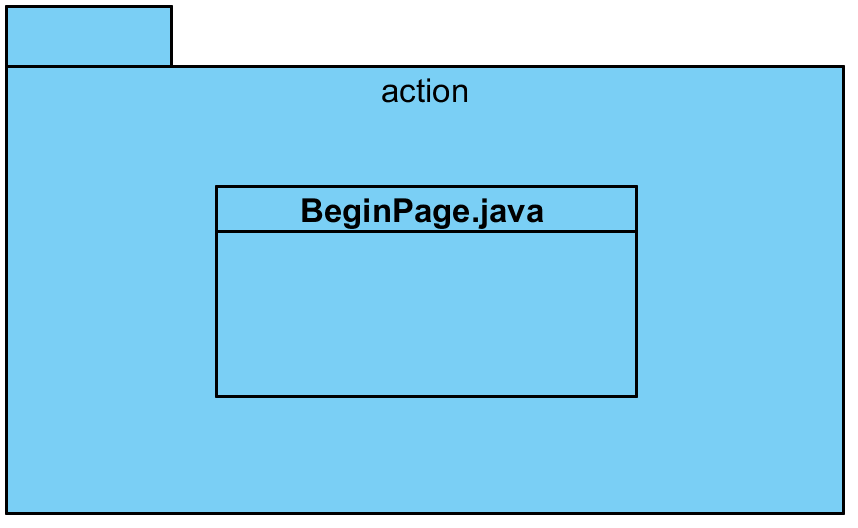
\includegraphics{diagrams/ActionPackageDiagram}
\end{figure}
Di seguito è riportata la tabella della descrizione della classe appartenente al package action:
\item \begin{tabular}{|p{7,6cm}|p{7,5cm}|}
	\hline
	\textbf{Classe} & \textbf{Descrizione}\\
	\hline
	BeginPage.java & Permette di avviare l'esecuzione del plug-in. \\
	\hline
\end{tabular}
	\end{description}	
		\subsubsection{Package parser}
		\begin{figure}[!h]
			\centering
			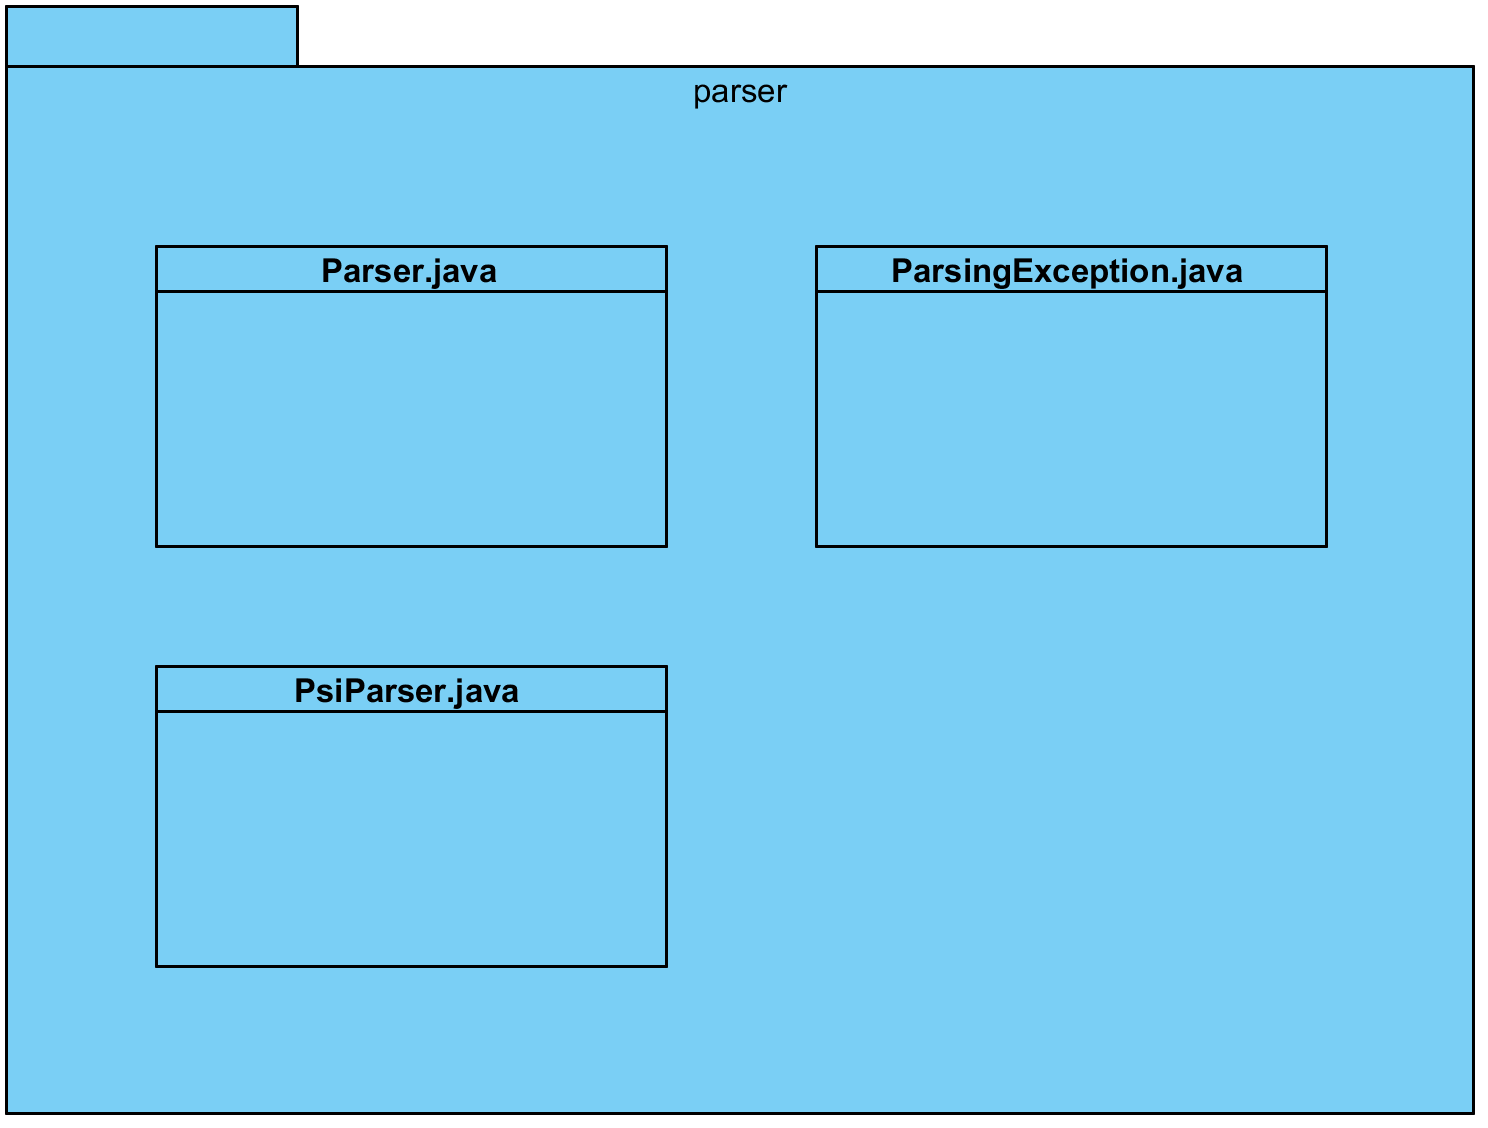
\includegraphics{diagrams/ParserPackageDiagram}
		\end{figure}
		\begin{description}
			\item Di seguito è riportata la tabella delle descrizioni delle classi e dell'interfaccia appartenenti al package parser:
			\item \begin{tabular}{|p{7,6cm}|p{7,5cm}|}
				\hline
				\textbf{Classe} & \textbf{Descrizione}\\
				\hline
				ParsingException.java & Permette di definire l'eccezione lanciata dal Parser.  \\
				\hline
				PsiParser.java & Permette di effettuare la conversione da Psi a Bean.\\
				\hline
			\end{tabular}
			\item \begin{tabular}{|p{7,6cm}|p{7,5cm}|}
				\hline
				\textbf{Interfaccia} & \textbf{Descrizione}\\
				\hline				Parser.java & Dichiara il metodo che  avvia il processo di conversione da Psi a Bean. \\
				\hline
			\end{tabular}
		\end{description}
			\subsubsection{Package refactor}
			Il sottopackage refactor si suddivide a sua volta in altri tre sottopackage, ossia:
			\begin{figure}[!h]
				\centering
				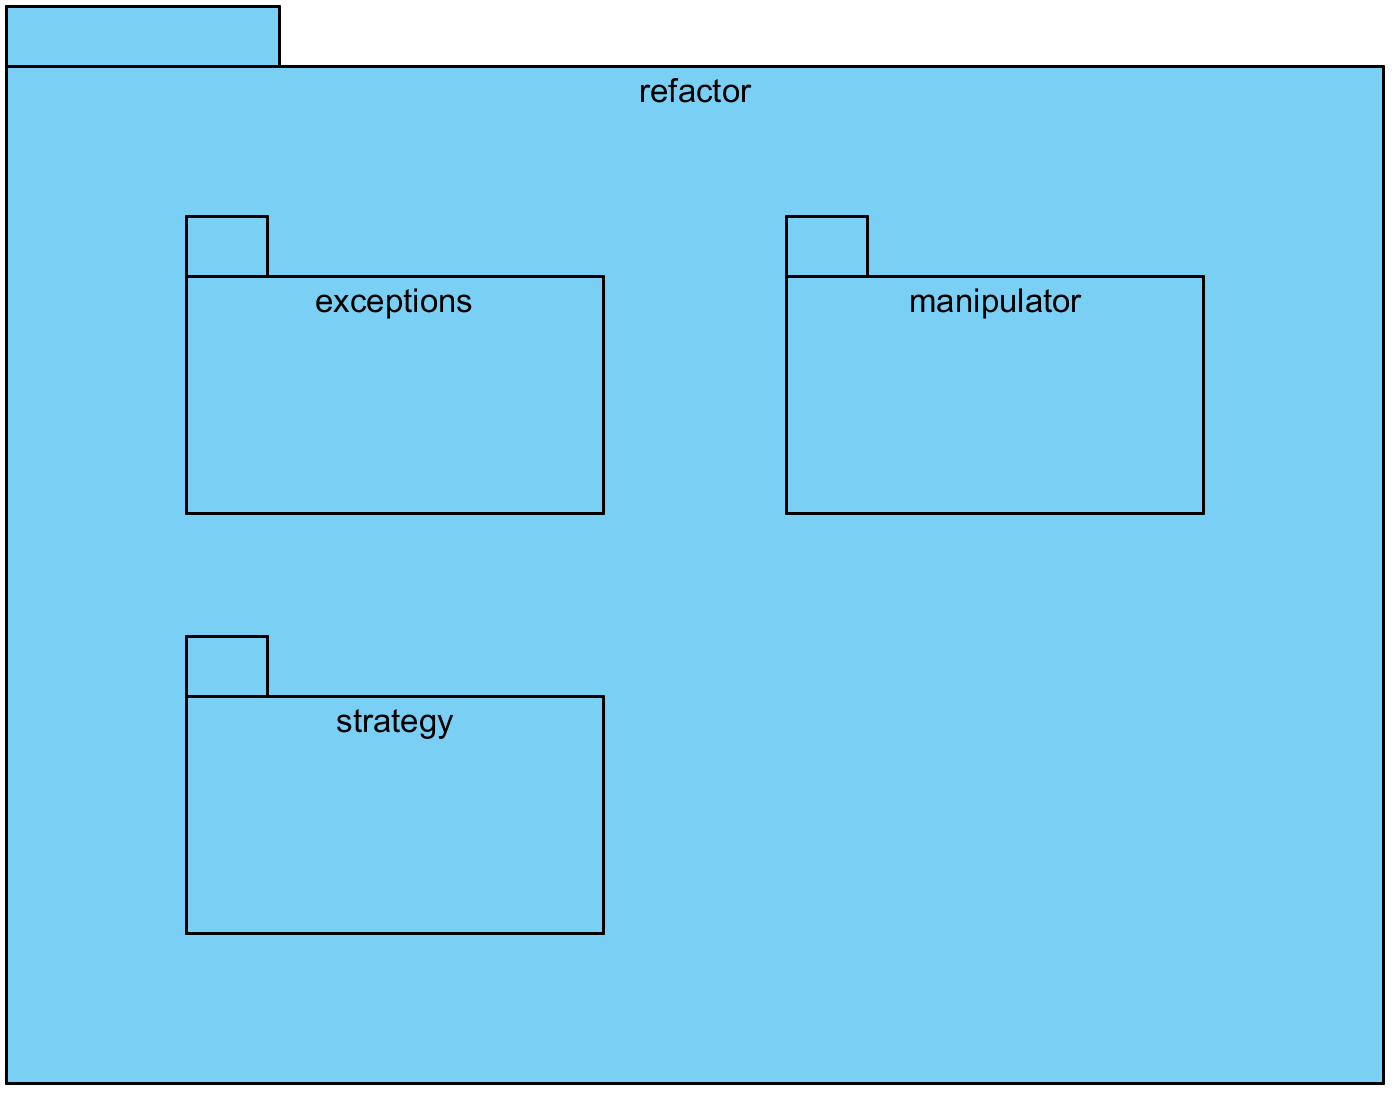
\includegraphics{diagrams/RefactorPackageDiagram}
			\end{figure}
			\begin{description}
				\newpage
				\item[ 2.1.4.1 Package exceptions]
				\item \begin{figure}[!h]
					\centering
					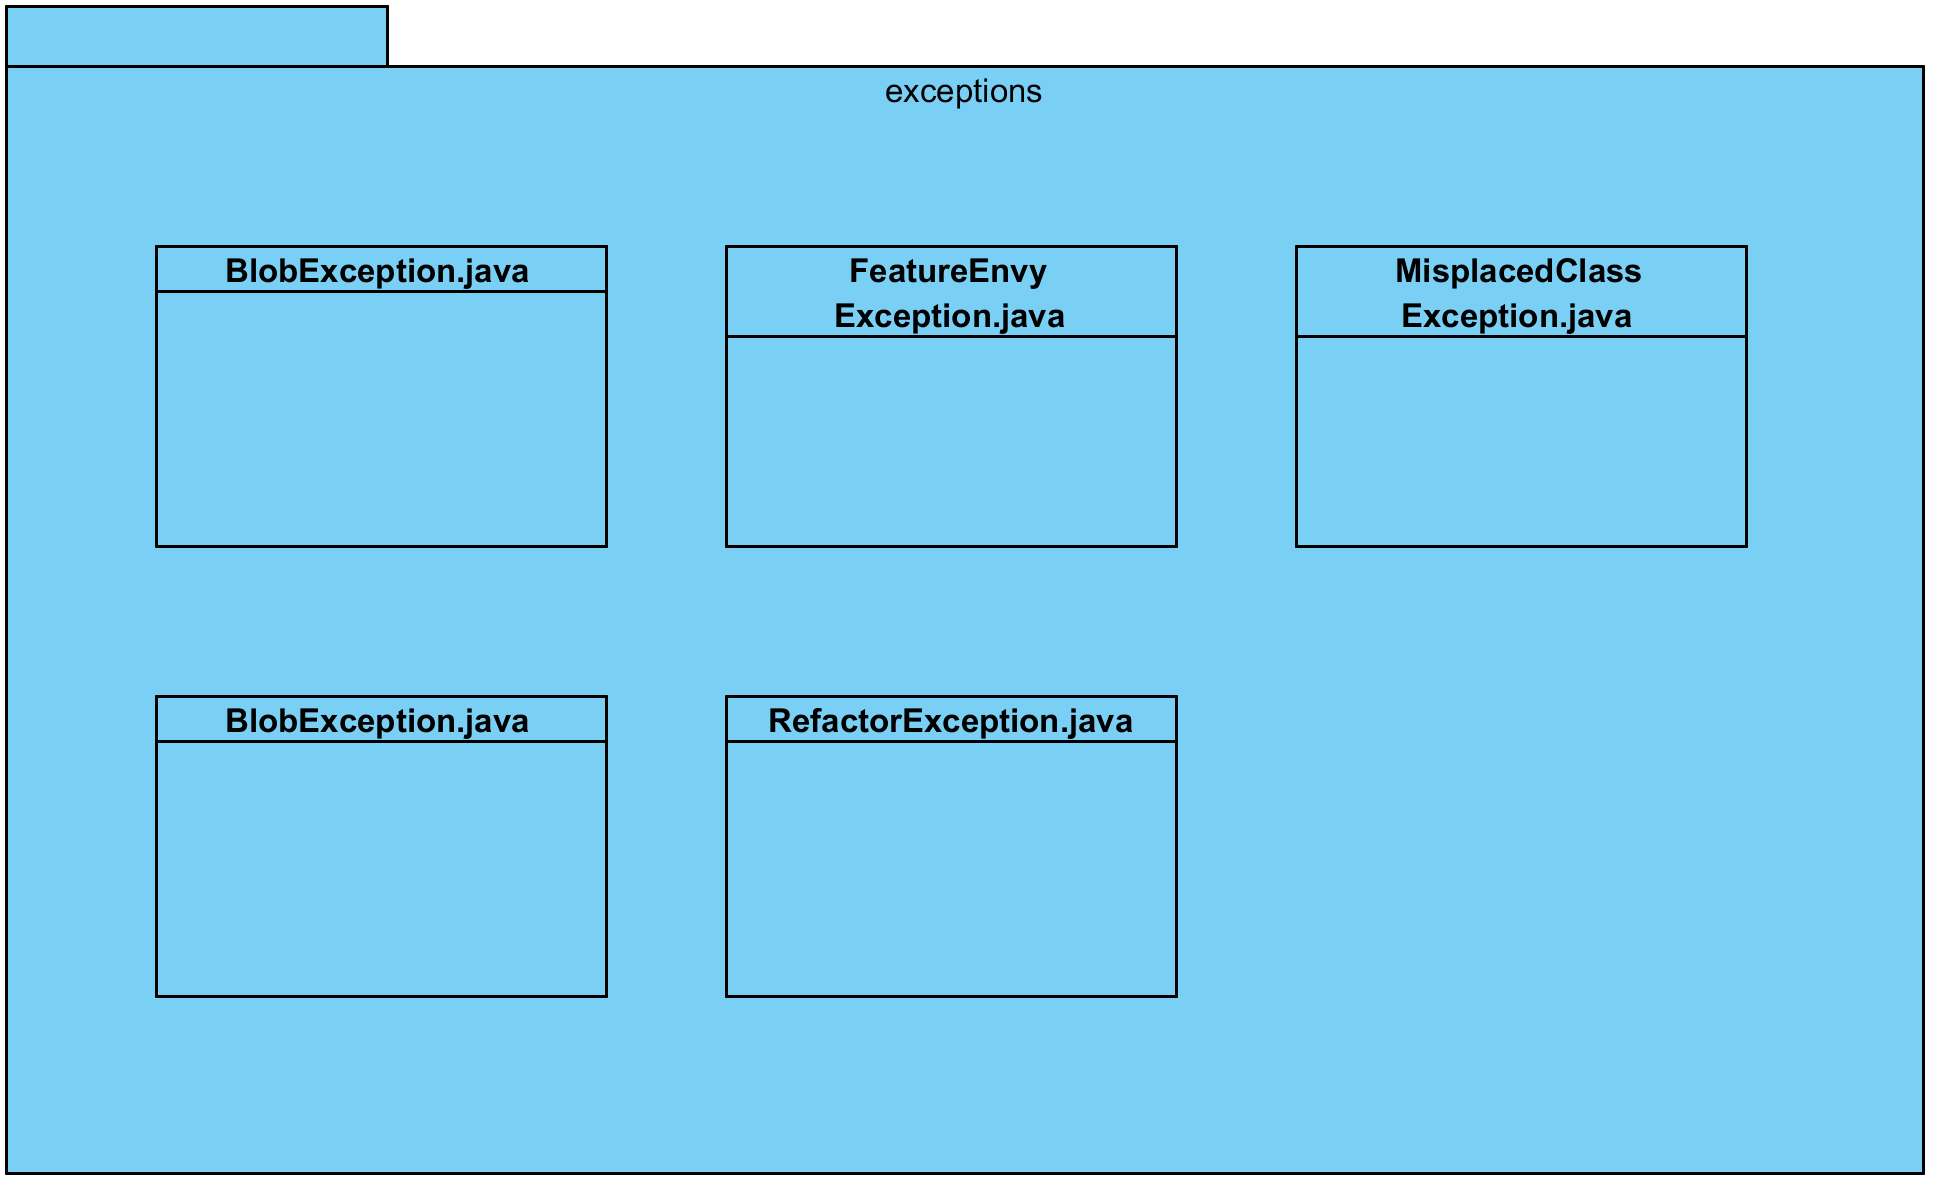
\includegraphics[width=15cm]{diagrams/ExceptionPackageDiagram}
				\end{figure}
				Di seguito è riportata la tabella delle descrizioni delle classi appartenenti al package exceptions:
				\item \begin{tabular}{|p{7,6cm}|p{7,5cm}|}
					\hline
					\textbf{Classe} & \textbf{Descrizione}\\
					\hline
					BlobException.java  & Permette di definire l'eccezione lanciata dallo Strategy riguardante il code smell Blob. \\
					\hline
					FeatureEnvyException.java  & Permette di definire l'eccezione lanciata dallo Strategy riguardante il code smell Feature Envy. \\
					\hline
					MisplacedClassException.java  & Permette di definire l'eccezione lanciata dallo Strategy riguardante il code smell Misplaced Class. \\
					\hline
					PromiscuousPackageException.java  & Permette di definire l'eccezione lanciata dallo Strategy riguardante il code smell Promiscuous Package. \\
					\hline
					RefactorException.java  & Permette di definire l'eccezione estesa dalle altre Exception già elencate. \\
					\hline
				\end{tabular}
				
				\item[ 2.1.4.2 Package manipulator]
				\item \begin{figure}[!h]
					\centering
					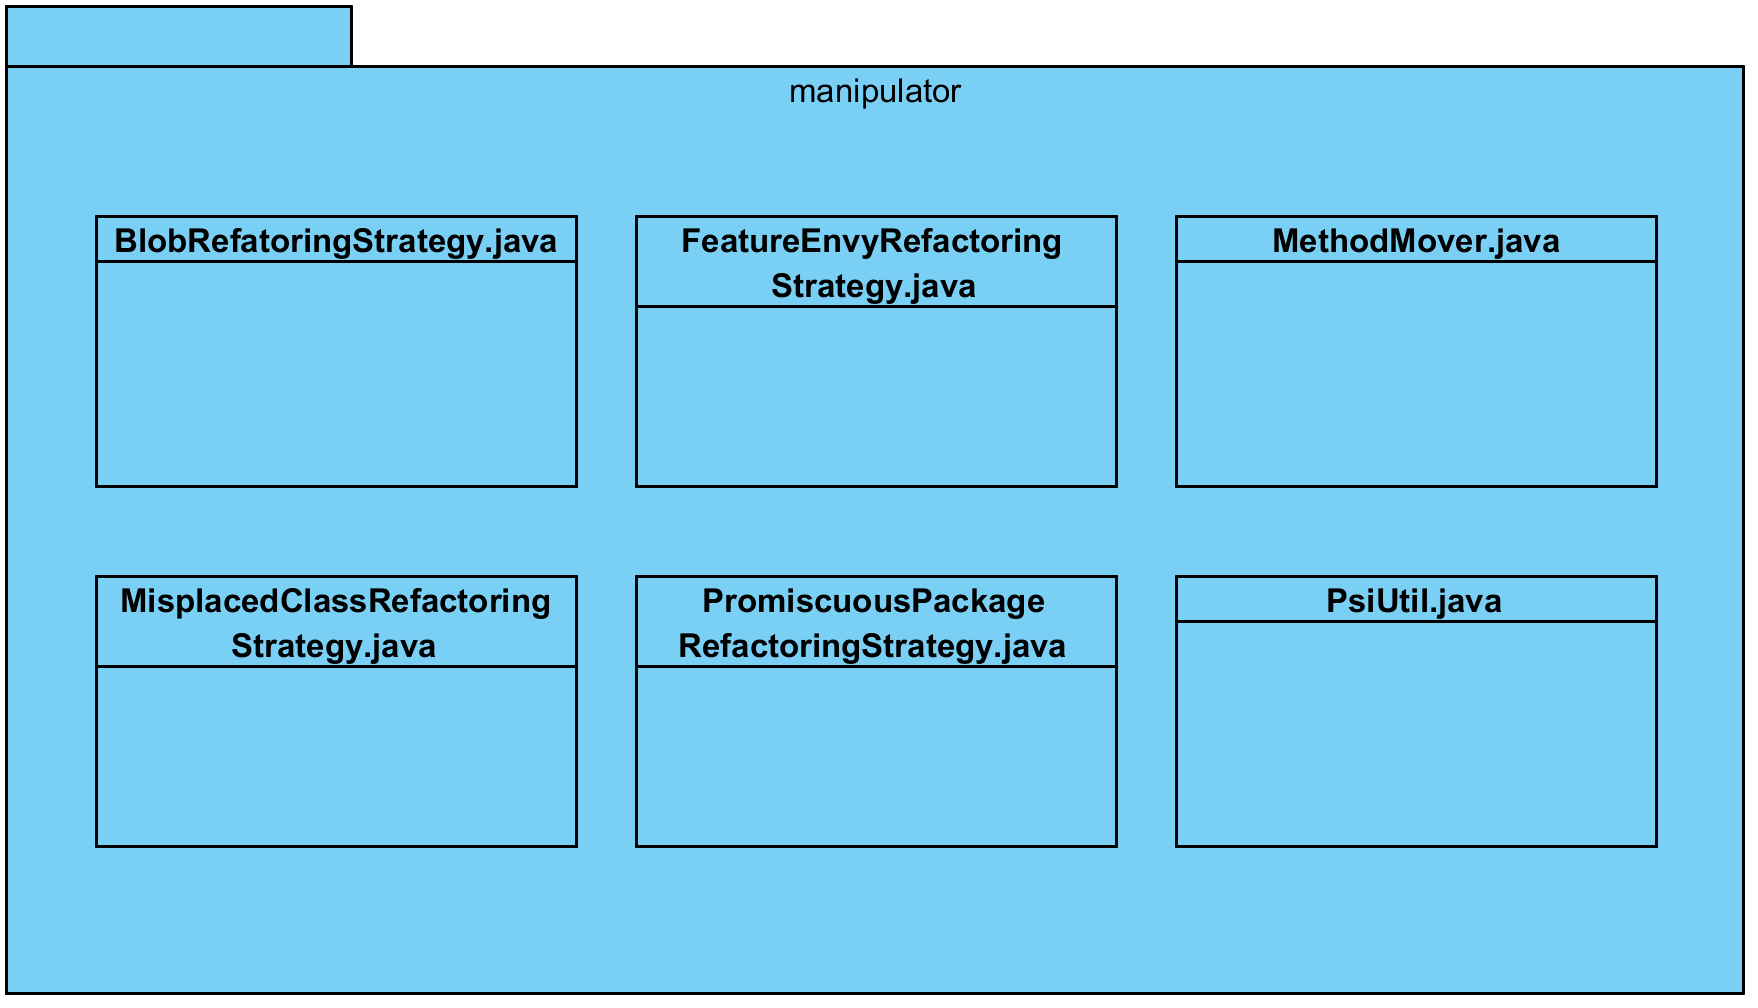
\includegraphics{diagrams/ManipulatorPackageDiagram}
				\end{figure}
				Di seguito è riportata la tabella delle descrizioni delle classi appartenenti al package manipulator:
				\item \begin{tabular}{|p{7,6cm}|p{7,5cm}|}
					\hline
					\textbf{Classe} & \textbf{Descrizione}\\
					\hline
					BlobRefatoringStrategy.java & Permette di effettuare il Refactor degli smell di tipo Blob. \\
					\hline
					FeatureEnvyRefactoringStrategy.java & Permette di effettuare il Refactor degli smell di tipo Feature Envy.\\
					\hline
					MethodMover.java & Permette di muovere un metodo in un'altra classe. \\
					\hline
					MisplacedClassRefactoringStrategy.java & Permette di effettuare il Refactor degli smell di tipo Misplaced Class. \\
					\hline
					PromiscuousPackageRefactoringStrategy.java & Permette di effettuare il Refactor degli smell di tipo Promiscuous Package. \\
					\hline
					PsiUtil.java & Permette di effettuare la conversione da Psi a Bean e viceversa. \\
					\hline
				\end{tabular}
				\item[ 2.1.4.3 Package strategy]
				\item \begin{figure}[!h]
					\centering
					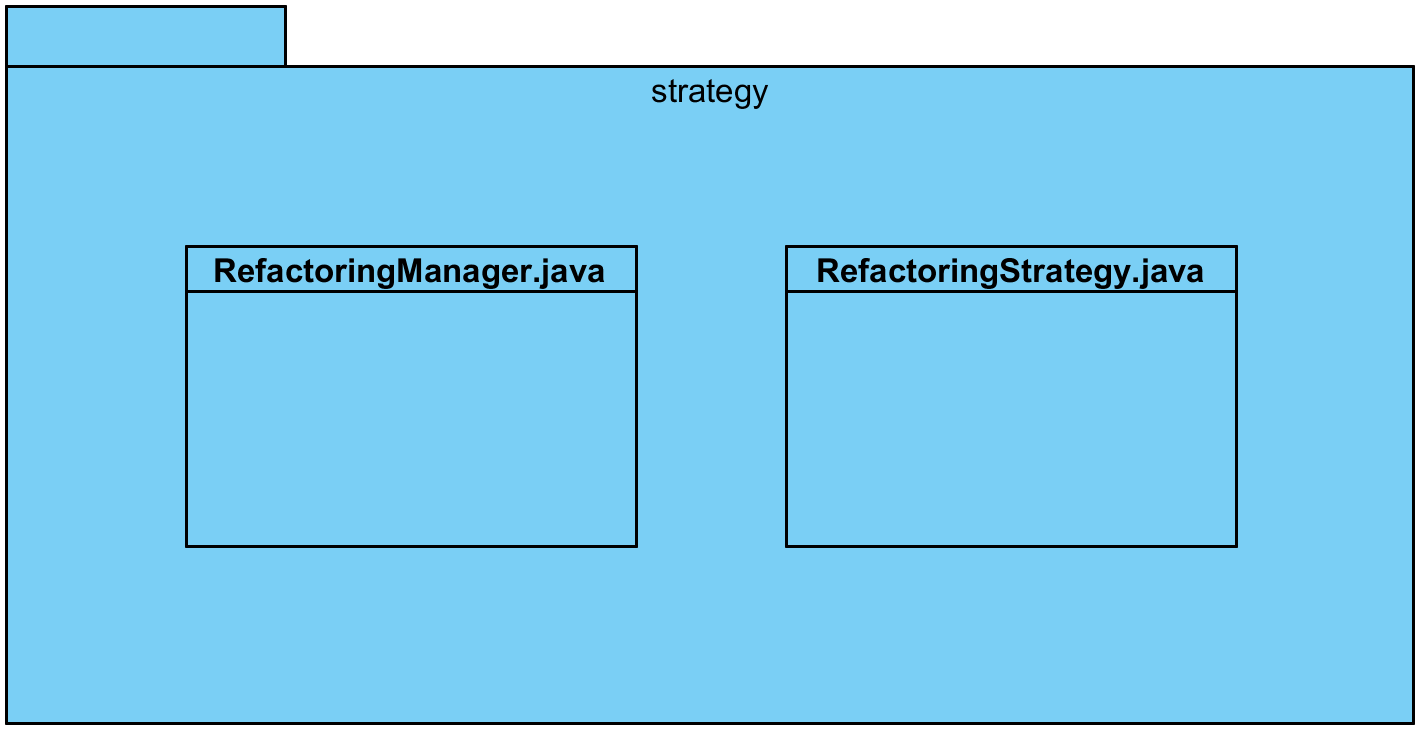
\includegraphics{diagrams/StrategyRefactorPackageDiagram}
				\end{figure}
				Di seguito sono riportate le tabelle delle descrizioni della classe e dell'interfaccia appartenenti al package strategy:
				\item \begin{tabular}{|p{7,6cm}|p{7,5cm}|}
					\hline
					\textbf{Classe} & \textbf{Descrizione}\\
					\hline
					RefactoringManager.java & Permette di effettuare il Refactor.  \\
					\hline
				\end{tabular}
				\item \begin{tabular}{|p{7,6cm}|p{7,5cm}|}
					\hline
					\textbf{Interfaccia} & \textbf{Descrizione}\\
					\hline
					RefactoringStrategy.java & Dichiara il metodo che effettua il Refactor, richiamato nella classe RefactoringManager. \\
					\hline
				\end{tabular}
				
			\end{description}
			
			\subsubsection{Package storage}
			Il sottopackage storage si suddivide a sua volta in tre sottopackage, ossia: 
			 \begin{figure}[!h]
				\centering
				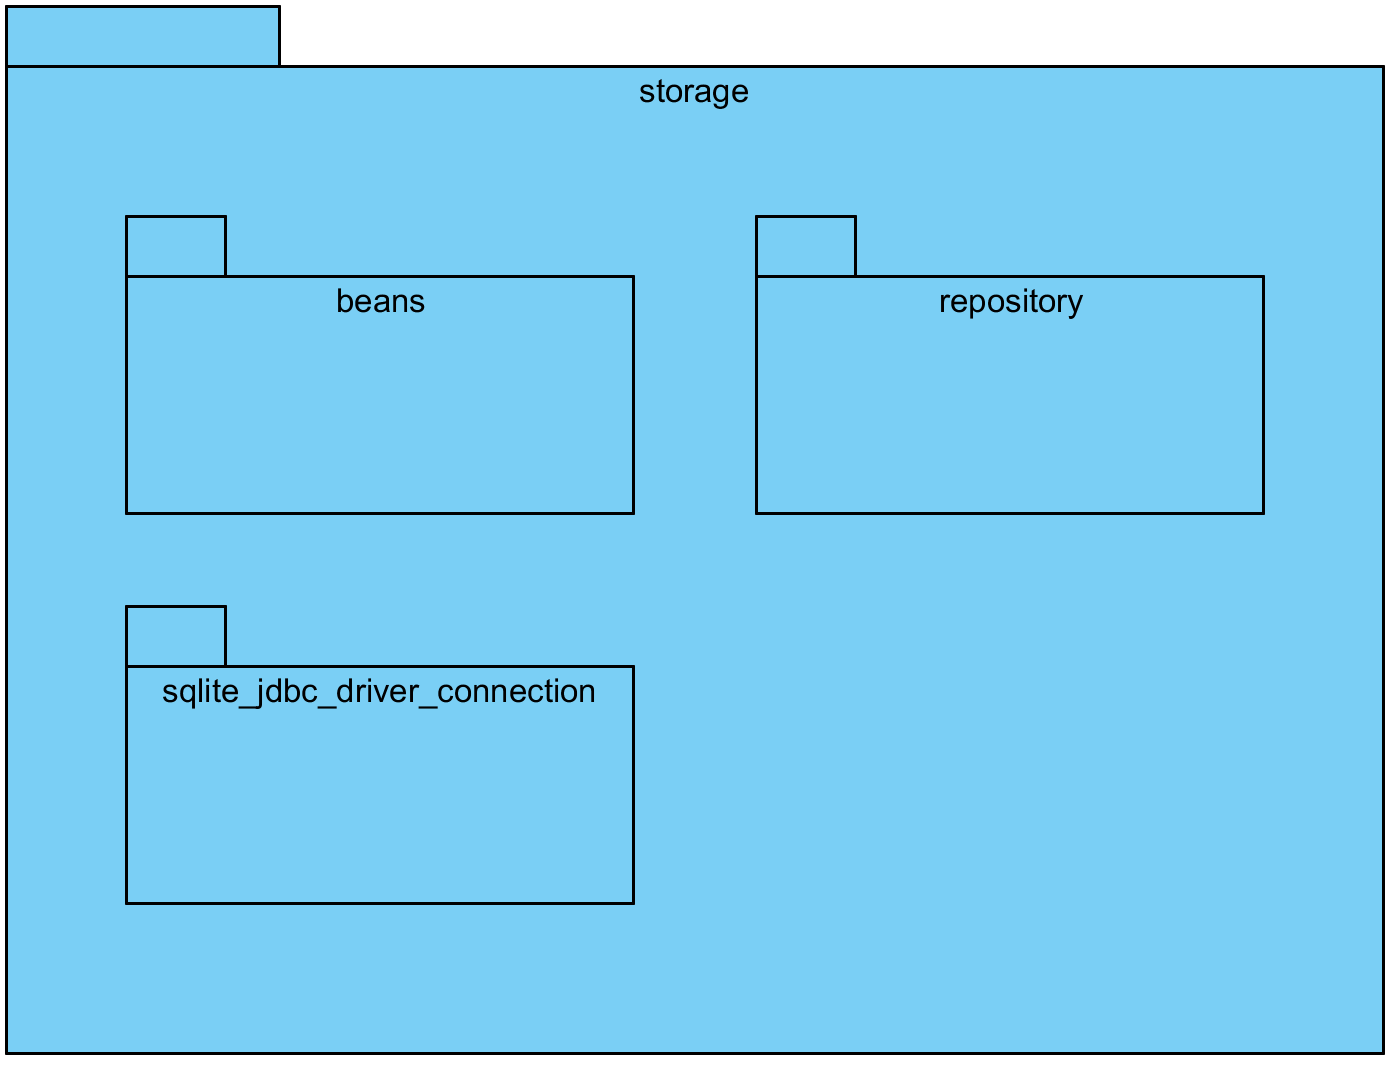
\includegraphics{diagrams/StoragePackageDiagram}
			\end{figure}
				\begin{description}
			\newpage
					\item[ 2.1.5.1 Package beans]
					\item \begin{figure}[!h]
						\centering
						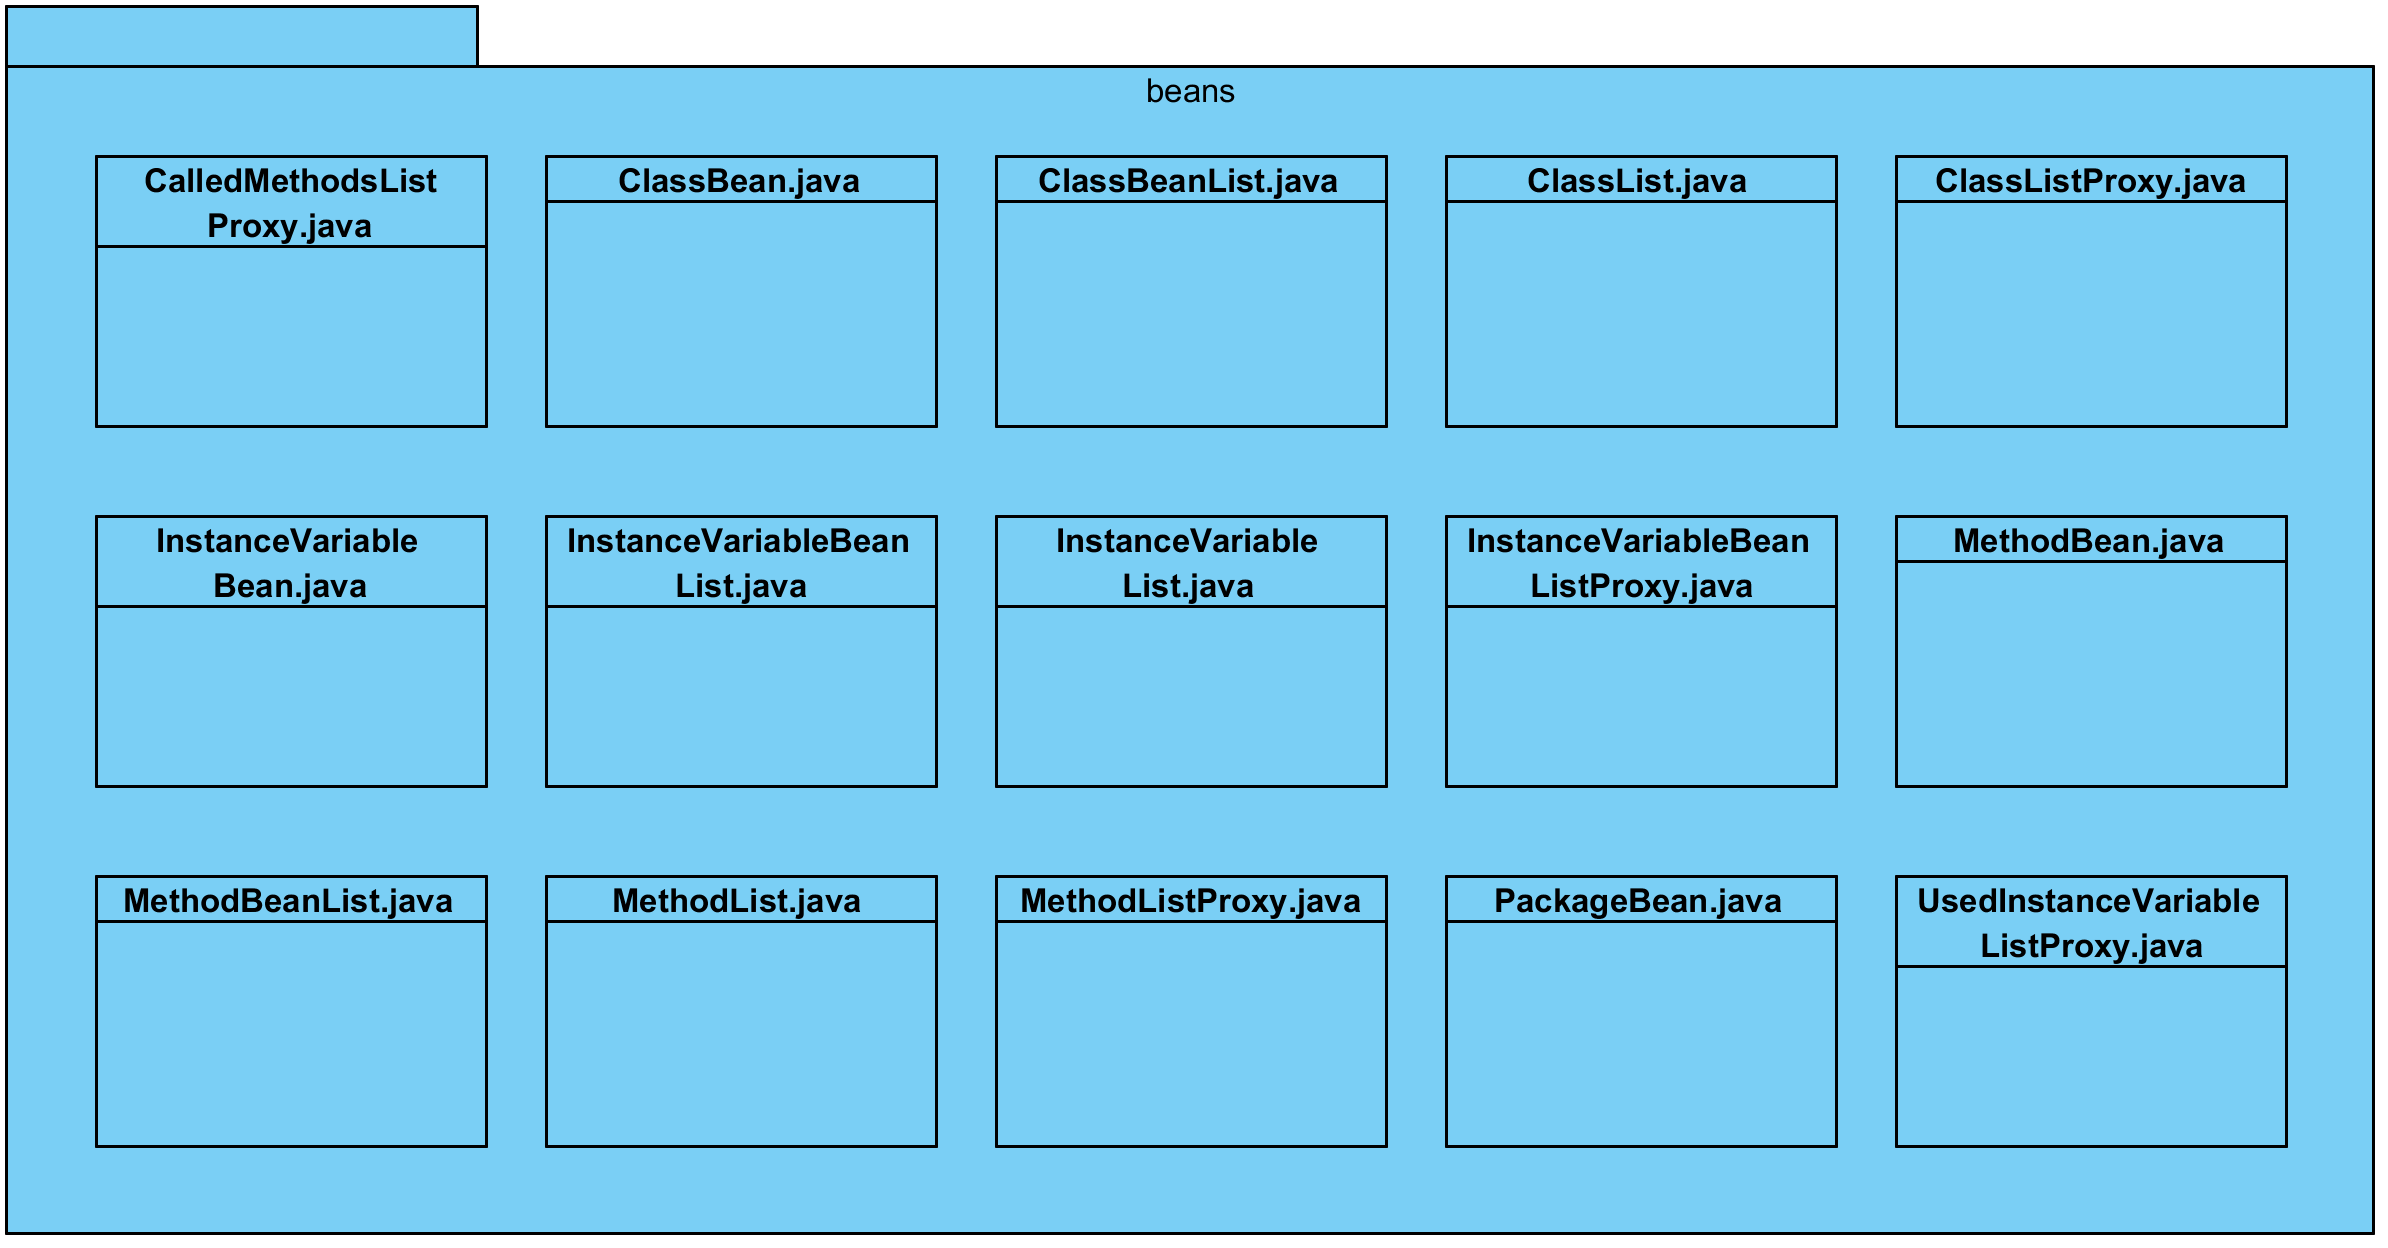
\includegraphics[width=15.5cm]{diagrams/BeansPackageDiagram}
					\end{figure}
					Di seguito sono riportate le tabelle delle descrizioni delle classi e delle interfacce appartenenti al package beans:
					\item \begin{tabular}{|p{7,6cm}|p{7,5cm}|}
						\hline
						\textbf{Classe} & \textbf{Descrizione}\\
						\hline
						CalledMethodsListProxy.java & Permette di realizzare il lazy loading della lista dei metodi chiamata da un metodo. \\
						\hline
						ClassBean.java & Permette di istanziare una classe. \\
						\hline
						ClassList.java & Permette di istanziare una lista di classi. \\
						\hline
						ClassListProxy.java & Permette di realizzare il lazy loading per le classi. \\
						\hline
						InstanceVariableBean.java & Permette di istanziare una variabile di istanza. \\
						\hline
						InstanceVariableList.java & Permette di istanziare una lista di variabili di istanza. \\
						\hline
						InstanceVariableListProxy.java & Permette di realizzare il lazy loading per le variabili di istanza. \\
						\hline
						MethodBean.java & Permette di istanziare un metodo. \\
						\hline
						MethodList.java & Permette di istanziare una lista di metodi. \\
						\hline
						MethodListProxy.java & Permette di realizzare il lazy loading per i metodi. \\
						\hline
						PackageBean.java & Permette di istanziare un package. \\
						\hline
						UsedInstanceVariableListProxy.java & Permette di realizzare il lazy loading delle variabili di istanza usate da un metodo. \\
						\hline
					\end{tabular}
				\item \begin{tabular}{|p{7,6cm}|p{7,5cm}|}
					\hline
					\textbf{Interfaccia} & \textbf{Descrizione}\\
					\hline
					ClassBeanList.java & Dichiara il metodo da implementare in ClassList e ClassListProxy. \\
					\hline
					InstanceVariableBeanList.java &  Dichiara il metodo da implementare in InstanceVariableList e InstanceVariableListProxy. \\
					\hline
					MethodBeanList.java & Dichiara il metodo da implementare in MethodList e MethodListProxy. \\
					\hline
				\end{tabular}
			\newpage
				\item[ 2.1.5.2 Package repository] 
				\item \begin{figure}[!h]
					\centering
					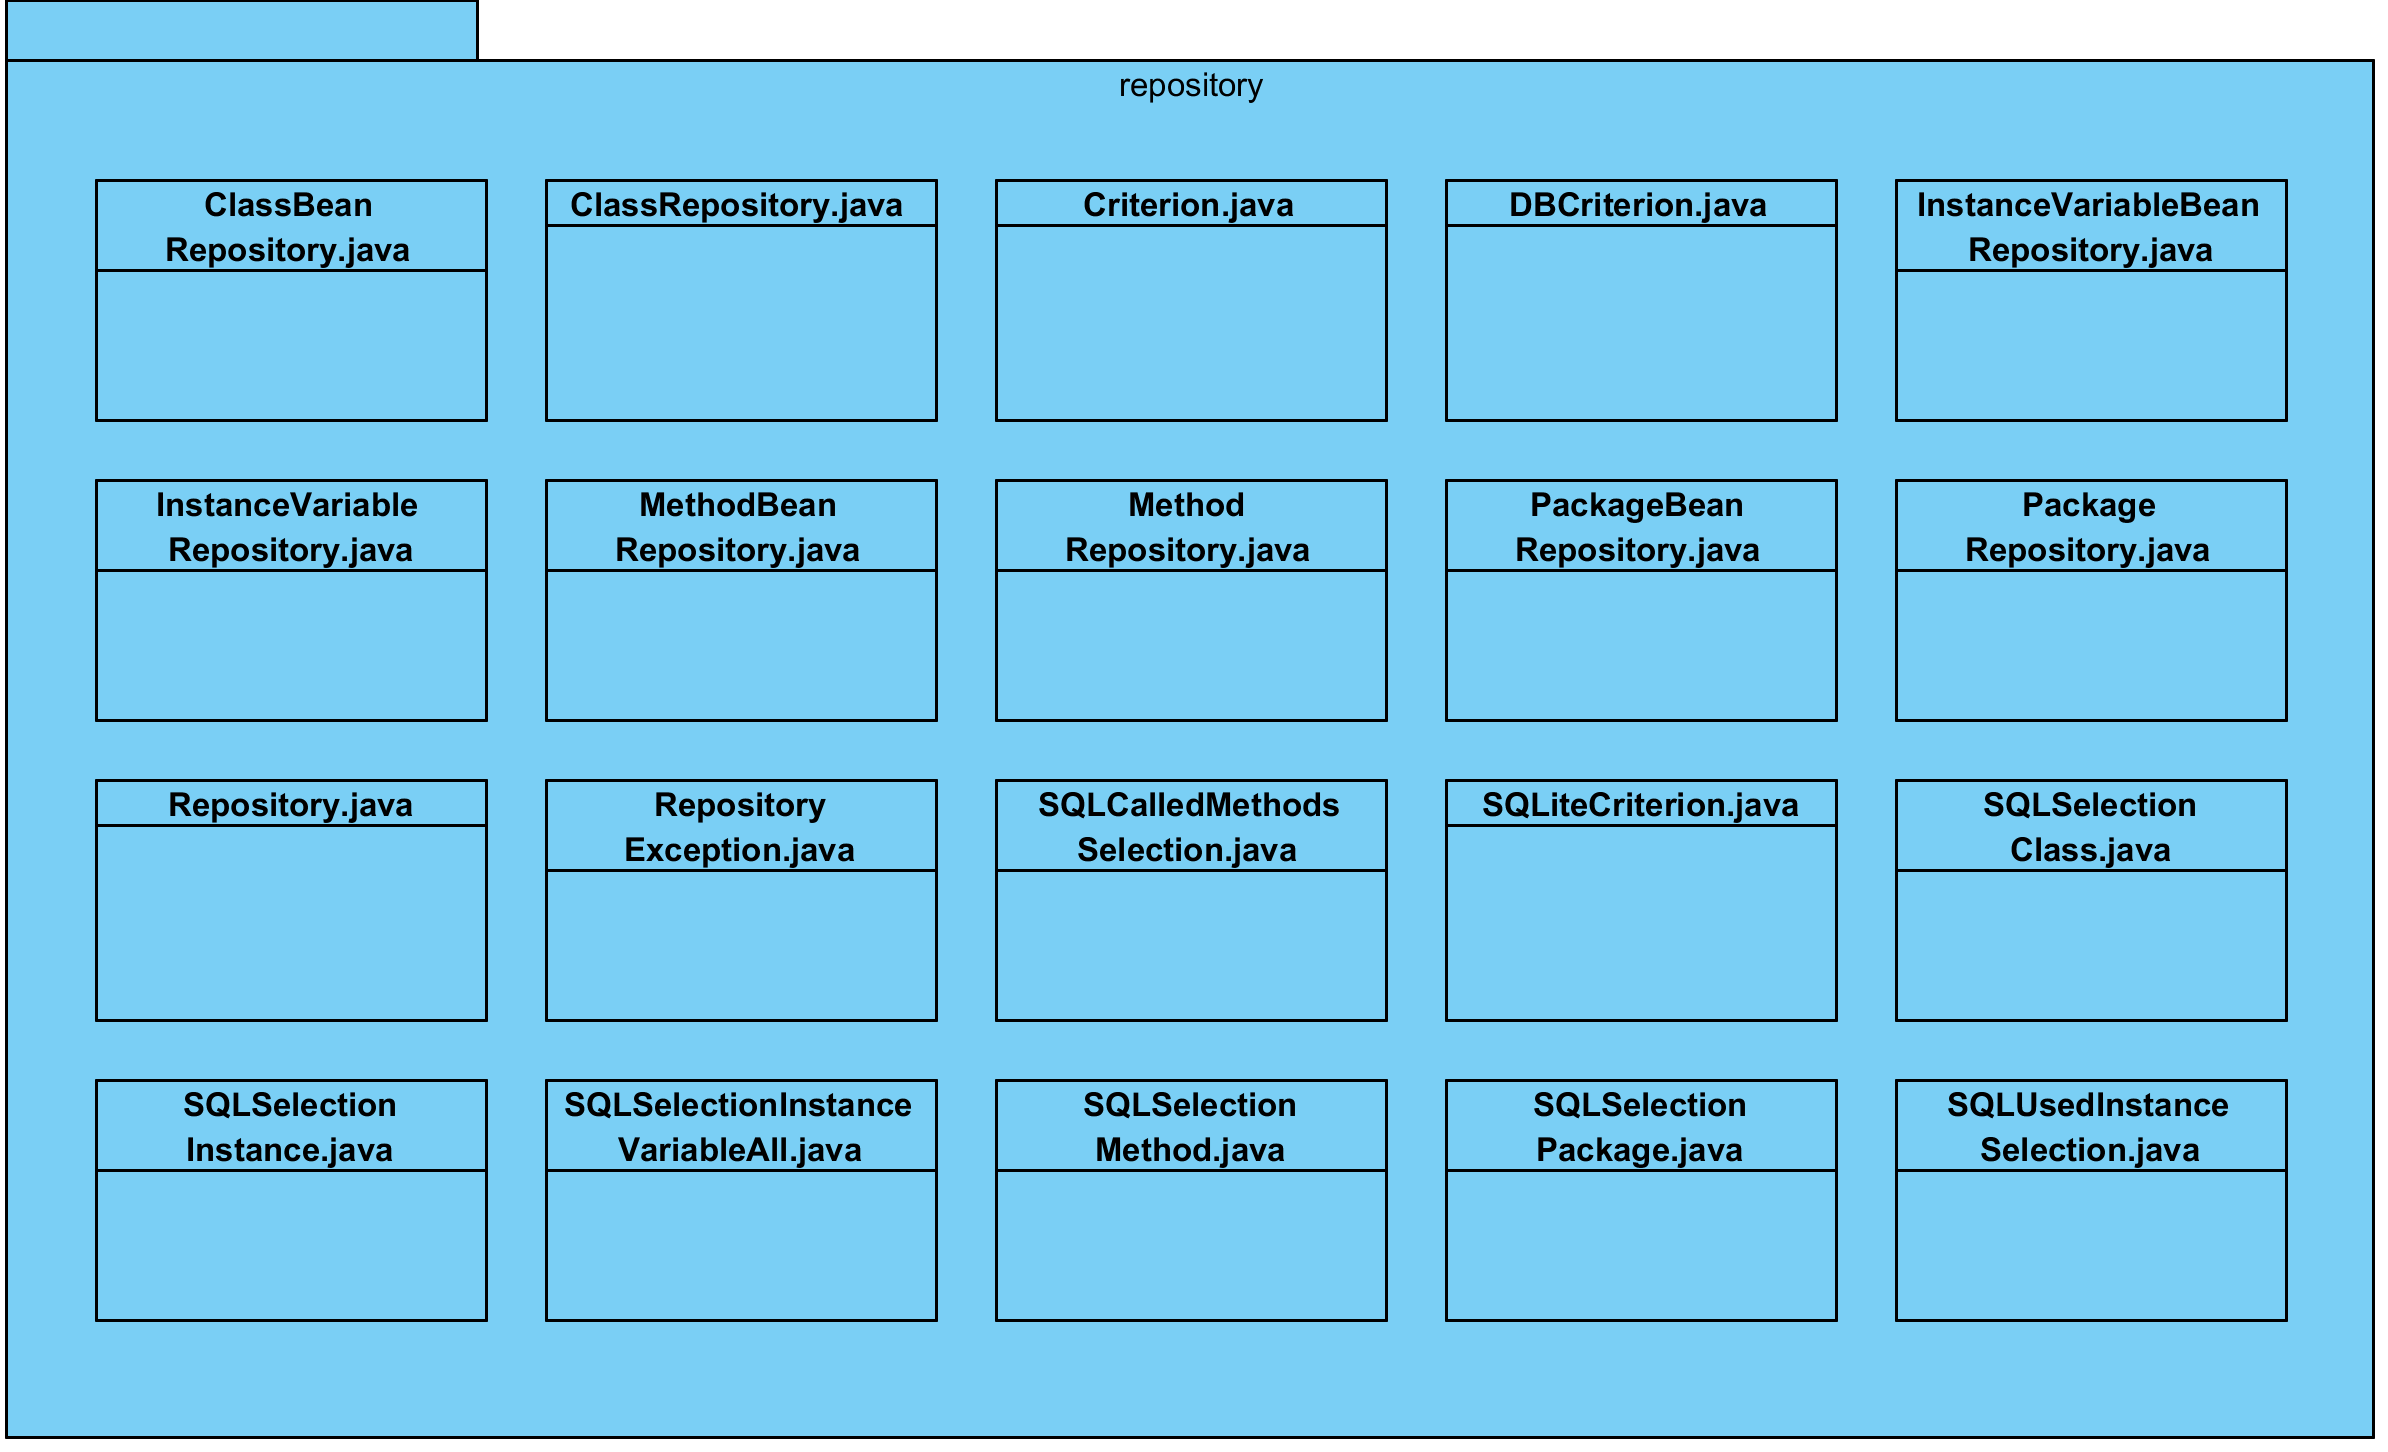
\includegraphics[width=15cm]{diagrams/RepositoryPackageDiagram}
				\end{figure}
				Di seguito sono riportate le tabelle delle descrizioni delle classi e delle interfacce appartenenti al package repository:
				\item \begin{tabular}{|p{7,6cm}|p{7,5cm}|}
					\hline
					\textbf{Classe} & \textbf{Descrizione}\\
					\hline
					ClassRepository.java & Permette di salvare nel DB le classi. \\
					\hline
					DBCreation.java & Permette di creare il DB. \\
					\hline
					InstanceVariableRepository.java & Permette di salvare nel DB le variabili di istanza.  \\
					\hline
					MethodRepository.java & Permette di salvare nel DB i metodi.  \\
					\hline
					PackageRepository.java & Permette di salvare nel DB i package. \\
					\hline
					RepositoryException.java & Permette di definire l'eccezione lanciata dalle Repository. \\
					\hline
					SQLCalledMethodsSelection.java & Permette di istanziare la query da eseguire per la selezione della lista dei metodi chiamata da un metodo. \\
					\hline
					SQLSelectionClass.java & Permette di istanziare la query da eseguire per la selezione delle classi. \\
					\hline
					SQLSelectionInstance.java & Permette di istanziare la query da eseguire per la selezione delle variabili di istanza. \\
					\hline
					SQLSelectionInstanceVariableAll.java & Permette di istanziare la query da eseguire per la selezione di tutte le variabili di istanza.\\
					\hline
					SQLSelectionMethod.java & Permette di istanziare la query da eseguire per la selezione dei metodi. \\
					\hline
					SQLSelectionPackage.java & Permette di istanziare la query da eseguire per la selezione dei package. \\
					\hline
					SQLUsedInstanceSelection.java & Permette di istanziare la query da eseguire per la selezione delle variabili di istanza usate da un metodo.	\\
					\hline
				\end{tabular}				
				\item \begin{tabular}{|p{7,6cm}|p{7,5cm}|}
					\hline
					\textbf{Interfaccia} & \textbf{Descrizione}\\
					\hline
					ClassBeanRepository.java & Dichiara i metodi da implementare nella Repository dedicata alle classi.\\
					\hline
					Criterion.java & Non dichiara nessun metodo, viene utilizzata per garantire manutenibilità. \\
					\hline
					InstanceVariableBeanRepository.java & Dichiara i metodi da implementare nella Repository dedicata alle variabili d'istanza. \\
					\hline
					MethodBeanRepository.java & Dichiara i metodi da implementare nella Repository dedicata ai metodi. \\
					\hline
					PackageBeanRepository.java & Dichiara i metodi da implementare nella Repository dedicata ai package. \\
					\hline
					Repository.java & Dichiara i metodi da implementare nelle interfacce dedicate alle Repository che la implementano.\\
					\hline	
					SQLiteCriterion.java & Dichiara il metodo da implementare
					nelle classi che istanziano le query per la selezione nel DB. \\
					\hline				
				\end{tabular}	
				\item[ 2.1.5.3 Package sqlite\_jdbc\_driver\_connection] 
				\item \begin{figure}[!h]
					\centering
					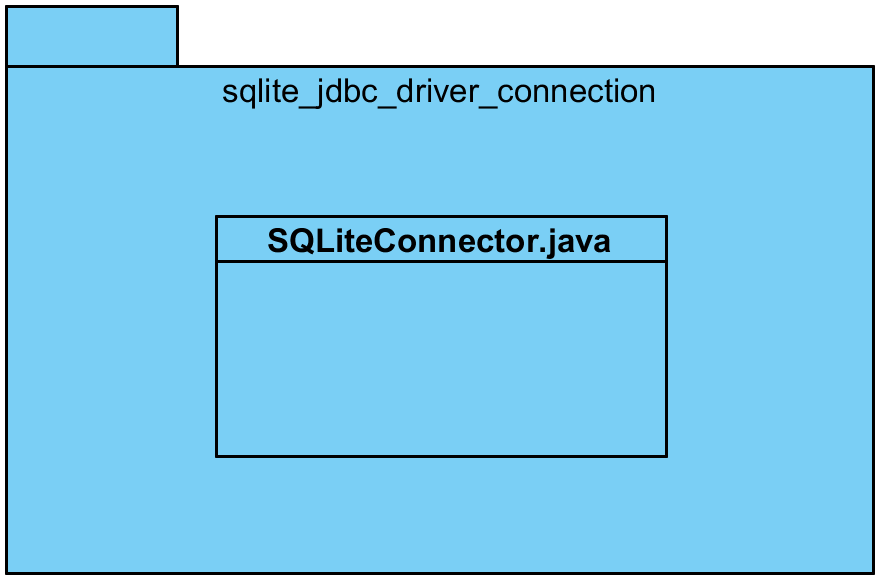
\includegraphics{diagrams/SQLite_JDBC_Driver_ConnectionPackageDiagram}
				\end{figure}
				Di seguito è riportata la tabella della descrizione della classe appartenente al package\\sqlite\_jdbc\_driver\_connection:
				\item \begin{tabular}{|p{7,6cm}|p{7,5cm}|}
					\hline
					\textbf{Classe} & \textbf{Descrizione}\\
					\hline
					SQLiteConnector.java & Permette di istanziare la connessione col DB. \\
					\hline
				\end{tabular}
			\end{description}
		
			\subsubsection{Package structuralMetrics}
			 \begin{figure}[!h]
				\centering
				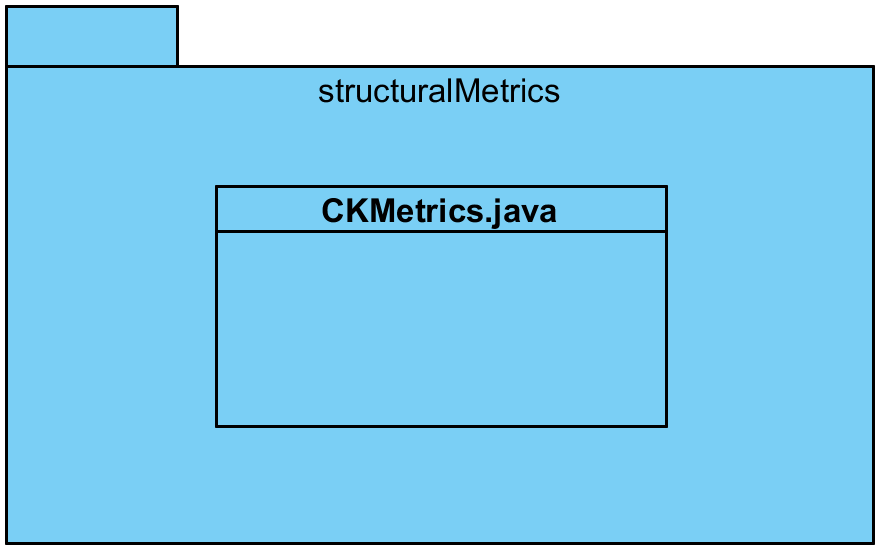
\includegraphics{diagrams/MetricsPackageDiagram}
			\end{figure}
			\begin{description}
				\item Di seguito è riportata la tabella della descrizione della classe appartenente al package\\structuralMetrics:
				\item \begin{tabular}{|p{7,6cm}|p{7,5cm}|}
					\hline
					\textbf{Classe} & \textbf{Descrizione}\\
					\hline
					CKMetrics.java & Permette di calcolare le metriche di qualità di un qualsiasi Bean. \\
					\hline
				\end{tabular}
			\end{description}
		\newpage
			\subsubsection{Package topics}
			 \begin{figure}[!h]
				\centering
				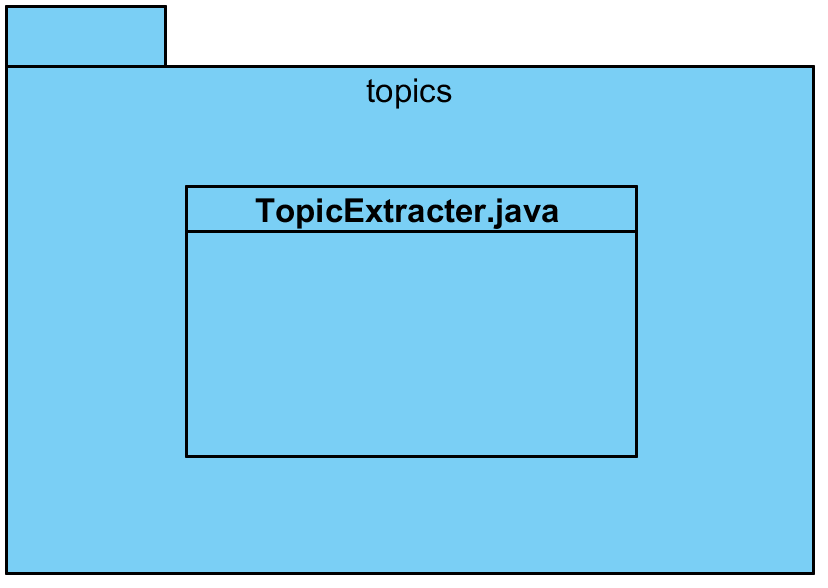
\includegraphics{diagrams/TopicsPackageDiagram}
			\end{figure}
	
			\begin{description}
				\item Di seguito è riportata la tabella della descrizione della classe appartenente al package\\topics:
				\item \begin{tabular}{|p{7,6cm}|p{7,5cm}|}
					\hline
					\textbf{Classe} & \textbf{Descrizione}\\
					\hline
					TopicExtracter.java & Permette di estrarre i topic, cioè cinque termini più frequenti, da un qualsiasi Bean. \\
					\hline
				\end{tabular}
			\end{description}
	
\newpage			
	\section{Interfaccia delle Classi}	
		\subsection{Analysis}
	
	
	\subsubsection{Code Smell}
	Si tratta di una classe che funge da interfaccia del sottosistema che individua i Code Smell durante l'analisi del codice.	
	\begin{itemize}
		\item  public abstract boolean affects(T component)\\
		Questo metodo verifica se è presente un Code Smell in un component T.
	\end{itemize}
	\begin{description}
		\item \textbf{ 3.1.1.1 Class Level Code Smell}
		\item Si tratta di una classe che funge da interfaccia del sottosistema che individua i Code Smell in una classe durante l'analisi del codice.		
		\begin{itemize}
			\item public boolean affects(ClassBean aBean)\\
			Questo metodo verifica se è presente un Code Smell in un Class Bean.
		\end{itemize}
		\item \textbf{ 3.1.1.2 Method Level Code Smell} 
		\item Si tratta di una classe che funge da interfaccia del sottosistema che individua i Code Smell in un metodo durante l'analisi del codice.		
		\begin{itemize}
			\item public boolean affects(MethodBean aMethod)\\
			Questo metodo verifica se è presente un Code Smell in un Method Bean.
		\end{itemize}
		\item \textbf{ 3.1.1.3 Package Level Code Smell}
		\item Si tratta di una classe che funge da interfaccia del sottosistema che individua i Code Smell in un package durante l'analisi del codice.		
		\begin{itemize}
			\item public boolean affects(PackageBean aPackage)\\
			Questo metodo verifica se è presente un Code Smell in un Package Bean.
		\end{itemize}
		\item \textbf{ 3.1.1.4 Blob Code Smell} 
		\item Si tratta di una classe che funge da interfaccia del sottosistema che individua i Code Smell di tipo Blob.		
		\begin{itemize}
			\item public boolean affects(ClassBean aClass)\\
			Questo metodo verifica se è presente un Code Smell di tipo Blob in un Class Bean.
		\end{itemize}
		\item \textbf{ 3.1.1.5 Feature Envy Code Smell}
		\item Si tratta di una classe che funge da interfaccia del sottosistema che individua i Code Smell di tipo Feature Envy.		
		\begin{itemize}
			\item public boolean affects(MethodBean aMethod)\\
			Questo metodo verifica se è presente un Code Smell di tipo Feature Envy in un Method Bean.
		\end{itemize}
		\item \textbf{ 3.1.1.6 Misplaced Class Code Smell} 
		\item Si tratta di una classe che funge da interfaccia del sottosistema che individua i Code Smell di tipo Misplaced Class.		
		\begin{itemize}
			\item public boolean affects(ClassBean aClass)\\
			Questo metodo verifica se è presente un Code Smell di tipo Misplaced Class in un Class Bean.
		\end{itemize}
		\item \textbf{ 3.1.1.7 Promiscuous Package Code Smell} 
		\item Si tratta di una classe che funge da interfaccia del sottosistema che individua i Code Smell di tipo Promiscuous Package.		
		\begin{itemize}
			\item public boolean affects(PackageBean aPackage)\\
			Questo metodo verifica se è presente un Code Smell di tipo Promiscuous Package in un Package Bean.
		\end{itemize}
\end{description}

	\subsubsection{Code Smell Detection}
			\begin{description}
			\item \textbf{3.1.2.1  Code Smell Detection Strategy}
			\item Si tratta di un'interfaccia del sottosistema che rileva Code Smell nei Bean.
			
			\begin{itemize}
				\item boolean isSmelly(T component)\\
				Questo metodo permette di verificare se il component T è affetto da Code Smell.				
			\end{itemize}
			\item \textbf{ 3.1.2.1.1  Class Smell Detection Strategy}\\
			Si tratta di un'interfaccia che implementa l'interfaccia del sottosistema che rilevano Code Smell nei Class Bean.
			\begin{itemize}
				\item public boolean isSmelly(ClassBean aClass)\\
				Questo metodo permette di verificare se un Class Bean è affetto da Code Smell.				
			\end{itemize}
			Questa interfaccia è implementata dalle classi \textbf{Textual Misplaced Class Strategy}, \textbf{Structural Misplaced Class Rule} e \textbf{Textual Blob Strategy}.
			\item \textbf{ 3.1.2.1.2  Method Smell Detection Strategy}\\
			Si tratta di un'interfaccia che implementa l'interfaccia del sottosistema che rilevano Code Smell nei Method Bean.
			\begin{itemize}
				\item public boolean isSmelly(MethodBean aMethod)\\
				Questo metodo permette di verificare se un Method Bean è affetto da Code Smell.				
			\end{itemize}
			Questa interfaccia è implementata dalla classe \textbf{Textual Feature Envy Strategy} e \textbf{Structural Feature Envy Rule}.
		
			\item \textbf{ 3.1.2.1.3  Package Smell Detection Strategy}\\
			Si tratta di un'interfaccia che implementa l'interfaccia del sottosistema che rilevano Code Smell nei Package Bean.		
			\begin{itemize}
				\item public boolean isSmelly(PackageBean aPackage)\\
				Questo metodo permette di verificare se un Package Bean è affetto da Code Smell.				
			\end{itemize}
			Questa interfaccia è implementata dalla classe \textbf{Textual Promiscuous Package Strategy}.
			
			\item \textbf{3.1.2.2 Comparable Bean}
			\item Si tratta di un'interfaccia del sottosistema che compara Bean fra loro per individuare Code Smell.
			\begin{itemize}
				\item  public double getSimilarity()\\
				Questo metodo permette di ottenere le similitudini dei Beans.		
			\end{itemize}
			\item \textbf{ 3.1.2.2.1 Bean Comparator}\\
			Si tratta di una classe che implementa l'interfaccia del sottosistema che compara Bean fra loro per individuare Code Smell.
			\begin{itemize}
				\item  public int compare(ComparableBean o1, ComparableBean o2)\\
				Questo metodo permette di comparare due Beans.		
			\end{itemize}
	\end{description}		
			
		\subsection{Parser}
		Si tratta di un'interfaccia del sottosistema che effettua la conversione in Bean.
		\begin{itemize}
			\item public void parse()\\Questo metodo effettua la conversione in Bean.
		\end{itemize}
		\subsubsection{Psi Parser}
		Si tratta di una classe che implementa l'interfaccia del sottosistema che effettua la conversione da Psi a Bean.
		\begin{itemize}
			\item public void parse()\\Questo metodo effettua la conversione da Psi a Bean.
		\end{itemize}
		
			
	
		\subsection{Refactoring}
	
		
			\subsubsection{Refactoring Manager}
			Si tratta di una classe che funge da interfaccia del sottosistema che esegue il Refactoring.
		\begin{itemize}
			
			\item public void executeRefactor()\\
			Questo metodo permette di eseguire il Refactor.
		\end{itemize}	
	
		\subsubsection{Refactoring Strategy}
		Si tratta di un'interfaccia del sottosistema che effettua il Refactoring.
		\begin{description}
			\item \begin{itemize}
				\item public void doRefactor()
			\end{itemize}
			Questo metodo permette di effettuare il Refactor.
			\item[3.4.2.1 Blob Refactoring Strategy]	
			\item Si tratta di una classe che implementa l'interfaccia del sottosistema che effettua il Refactoring del Code Smell Blob.
			\begin{itemize}
				\item public void doRefactor()\\Questo metodo permette di effettuare il Refactor delle classi affette da Code Smell di tipo Blob.
			\end{itemize}
			\item[3.4.2.2 Feature Envy Refactoring Strategy]	
			\item Si tratta di una classe che implementa l'interfaccia del sottosistema che effettua il Refactoring del Code Smell Feature Envy.
			\begin{itemize}
				\item public void doRefactor()\\Questo metodo permette di effettuare il Refactor delle metodi affetti da Code Smell di tipo Feature Envy.
			\end{itemize}
			\item[3.4.2.3 Misplaced Class Refactoring Strategy]
			\item Si tratta di una classe che implementa l'interfaccia del sottosistema che effettua il Refactoring del Code Smell Misplaced Class.
			 \begin{itemize}
				\item public void doRefactor()\\Questo metodo permette di effettuare il Refactor delle classi affette da Code Smell di tipo Misplaced Class.
			\end{itemize}
			\item[3.4.2.4 Promiscuous Package Refactoring Strategy]	
			\item Si tratta di una classe che implementa l'interfaccia del sottosistema che effettua il Refactoring del Code Smell Promiscuous Package.
			\begin{itemize}
				\item public void doRefactor()\\Questo metodo permette di effettuare il Refactor dei package affetti da Code Smell di tipo Promiscuous Package.
				
			\end{itemize}	
		\end{description}
		
			
			
			\subsection{Storage}
			
			\subsubsection{Beans}
			\begin{description}
				\item \textbf{3.1.1.1  Package Bean}
				\item Si tratta di una classe che funge da interfaccia del sottosistema che immagazzina i Package Bean.
				
				\begin{itemize}
					\item public boolean isAffected(CodeSmell smell)\\
					Questo metodo permette di verificare se nel Package Bean è presente un code smell.
					\item public void addClassList(ClassBean bean)\\
					Questo metodo permette di aggiungere una classe al Package Bean.
					\item public void removeClassList(ClassBean bean)\\
					Questo metodo permette di rimuovere una classe dal Package Bean.
					\item public void addSmell(CodeSmell smell)\\
					Questo metodo permette di aggiungere un code smell al Package Bean.				
				\end{itemize}
				\newpage
				\item \textbf{3.1.1.2  Class Bean} 
				\item Si tratta di una classe che funge da interfaccia del sottosistema che immagazzina i Class Bean. 
				
				\begin{itemize}
					\item public boolean isAffected(CodeSmell smell)\\
					Questo metodo permette di verificare se nel Class Bean è presente un code smell.
					\item public void addInstanceVariableList(ClassBean bean)\\
					Questo metodo permette di aggiungere una variabile d'istanza alla lista delle variabili d'istanza del Class Bean.
					\item public void removeInstanceVariableList(ClassBean bean)\\
					Questo metodo permette di rimuovere una variabile d'istanza alla lista delle variabili d'istanza del Class Bean.
					\item public void addMethodBeanList(MethodBean bean)\\
					Questo metodo permette di aggiungere un metodo alla lista dei metodi appartenenti al Class Bean.
					\item public void removeMethodBeanList(MethodBean bean)\\
					Questo metodo permette di rimuovere un metodo alla lista dei metodi appartenenti al Class Bean.
					\item public void addImports(String i)\\
					Questo metodo permette di aggiungere un import al Class Bean.
					\item public void removeImports(String i)\\
					Questo metodo permette di rimuovere un import dal Class Bean.
					\item public void addSmell(CodeSmell smell)\\
					Questo metodo permette di aggiungere un code smell al Class Bean.	 
				\end{itemize}
				
				\item \textbf{3.1.1.3  Method Bean} 
				
				\item Si tratta di una classe che funge da interfaccia del sottosistema che immagazzina i Method Bean. 
				
				\begin{itemize}
					\item public boolean isAffected(CodeSmell smell)\\
					Questo metodo permette di verificare se nel Method Bean è presente un code smell.
					\item public void addParameters(String key, ClassBean bean)\\
					Questo metodo permette di aggiungere un paramentro al Method Bean.
					\item public void removeParameters(String key, ClassBean bean)\\
					Questo metodo permette di rimuovere un paramentro al Method Bean.
					\item public void addInstanceVariableList(InstanceVariableBean bean)\\
					Questo metodo permette di aggiungere una variabile d'istanza alla lista delle variabili d'istanza del Method Bean.
					\item public void removeInstanceVariableList(InstanceVariableBean bean)\\
					Questo metodo permette di rimuovere una variabile d'istanza alla lista delle variabili d'istanza del Method Bean.
					\item  public void addMethodsCalls(MethodBean bean)\\
					Questo metodo permette di aggiungere un Method Bean alla lista dei metodi chiamati.
					\item public void removeMethodsCalls(MethodBean bean)\\
					Questo metodo permette di rimuovere un Method Bean alla lista dei metodi chiamati.
					\item public void addSmell(CodeSmell smell)\\
					Questo metodo permette di aggiungere un code smell al Method Bean.		 
				\end{itemize}
			\item \textbf{3.1.1.4  Class Bean List} 
			\item Si tratta di un'interfaccia del sottosistema che contiene la lista di Class Bean. 
			
			\begin{itemize}
				\item public List<ClassBean> getList()\\
				Questo metodo permette di ottenere la lista di classi presenti nel DB.
				
			\end{itemize}
				\item \textbf{ 3.1.1.4.1  Class List} \\
				Si tratta di una classe che implementa l'interfaccia del sottosistema che crea la lista di Class Bean.
				
				\begin{itemize}
					\item public List<ClassBean> getList() \\
					Questo metodo permette di ottenere la lista di classi presenti nel DB.
					\item public void setList(List<ClassBean> classes)\\
					Questo metodo permette di settare la lista di classi.
				\end{itemize}
			
				\item \textbf{ 3.1.1.4.2  Class List Proxy} \\
				Si tratta di una classe che implementa l'interfaccia del sottosistema che si occupa del lazy loading delle classi.
				
				\begin{itemize}
					\item public List<ClassBean> getList() \\
					Questo metodo permette di ottenere la lista di classi presenti nel DB.
				\end{itemize}
				
				\item \textbf{3.1.1.5  Method Bean List} 
			
			\item Si tratta di un'interfaccia del sottosistema che contiene la lista di Method Bean. 
			
			\begin{itemize}
				\item public List<MethodBean> getList() \\
				Questo metodo permette di ottenere la lista di metodi presenti nel DB.
			\end{itemize}
				\item \textbf{ 3.1.1.5.1  Method List} \\
				Si tratta di una classe che implementa l'interfaccia del sottosistema che crea la lista di Method Bean.
				
				\begin{itemize}
					\item public List<MethodBean> getList() \\
					Questo metodo permette di ottenere la lista di metodi presenti nel DB.
					\item public void setList(List<MethodBean> classes)\\
					Questo metodo permette di settare la lista di metodi.
				\end{itemize}
			\item \textbf{ 3.1.1.5.2  Method List Proxy} \\
			Si tratta di una classe che implementa l'interfaccia del sottosistema che si occupa del lazy loading dei metodi.
			
			\begin{itemize}
				\item public List<MethodBean> getList() \\
				Questo metodo permette di ottenere la lista di metodi presenti nel DB.
			\end{itemize}
			
			\item \textbf{ 3.1.1.5.3  Called Methods List Proxy} \\
			Si tratta di una classe che implementa l'interfaccia del sottosistema che si occupa del lazy loading dei metodi.
			
			\begin{itemize}
				\item public List<MethodBean> getList() \\
				Questo metodo permette di ottenere la lista di metodi chiamati da uno specifico metodo.
			\end{itemize}
		
				\item \textbf{3.1.1.6  Instance Variable Bean List} 
				\item Si tratta di un'interfaccia del sottosistema che contiene la lista di Instance Variable Bean.
				
				\begin{itemize}
					\item public List<InstanceVariableBean> getList()\\
					Questo metodo permette di ottenere la lista di variabili di istanza presenti nel DB.
				\end{itemize}
				\item \textbf{ 3.1.1.6.1  Instance Variable List} \\
				Si tratta di una classe che implementa l'interfaccia del sottosistema che crea la lista di Instance Variable Bean.
				\begin{itemize}
					\item public List<InstanceVariableBean> getList() \\
					Questo metodo permette di ottenere la lista di variabili di istanza presenti nel DB.
					\item public void setList(List<InstanceVariableBean> classes)\\
					Questo metodo permette di settare la lista di variabili di istanza.
				\end{itemize}
				\item \textbf{ 3.1.1.6.2  Instance Variable List Proxy} \\
				Si tratta di una classe che implementa l'interfaccia del sottosistema che si occupa del lazy loading delle variabili di istanza.
				
				\begin{itemize}
					\item public List<InstanceVariableBean> getList() \\
					Questo metodo permette di ottenere la lista di variabili di istanza presenti nel DB.
				\end{itemize}
				
					\item \textbf{ 3.1.1.6.3  Used Instance Variable List Proxy} \\
				Si tratta di una classe che implementa l'interfaccia del sottosistema che si occupa del lazy loading delle variabili di istanza.
				
				\begin{itemize}
					\item public List<InstanceVariableBean> getList() \\
					Questo metodo permette di ottenere la lista delle variabili di istanza utilizzate da uno specifico metodo.
				\end{itemize}		
			
			
			
			\end{description}
			
			
			
			\subsubsection{Repository}
				Si tratta di una classe che funge da interfaccia del sottosistema che contiene la Repository dei Bean.	
			\begin{itemize}
					\item public void add(T toAdd)\\
				Questo metodo permette di aggiungere un Bean al DB.
				\item public void remove(T toRemove)\\
				Questo metodo permette di rimuovere un Bean dal DB. 
				\item public void update(T toUpdate) \\
				Questo metodo permette di aggiornare un Bean contenuto nel DB.
				\item public List<T> select(Criterion criterion)\\
				Questo metodo permette di selezionare una lista di Bean dal DB.
			\end{itemize}
			\begin{description}
				\item \textbf{3.1.2.1  Package Bean Repository}
				
				Si tratta di una classe che funge da interfaccia del sottosistema che contiene la Repository dei Package Bean.
				
				\begin{itemize}
					\item public void add(PackageBean aPackage)\\
					Questo metodo permette di aggiungere un Package Bean al DB.
					\item public void remove(PackageBean aPackage)\\
					Questo metodo permette di rimuovere un Package Bean dal DB. 
					\item public void update(PackageBean aPackage) \\
					Questo metodo permette di aggiornare un Package Bean contenuto nel DB.
					\item public List<PackageBean> select(Criterion criterion)\\
					Questo metodo permette di selezionare una lista di Package Bean dal DB.
				\end{itemize}
				Questa interfaccia viene implementata dalla classe \textbf{Package Repository}.
				\item \textbf{3.1.2.2  Class Bean Repository}
				
				Si tratta di un'interfaccia del sottosistema che contiene la repository dei class bean.
				
				\begin{itemize}
					\item public void add(ClassBean aClass)\\
					Questo metodo permette di aggiungere un Class Bean al DB.
					\item public void remove(ClassBean aClass)\\
					Questo metodo permette di rimuovere un Class Bean dal DB.  
					\item public void update(ClassBean aClass) \\
					Questo metodo permette di aggiornare un Class Bean contenuto nel DB.
					\item public List<ClassBean> select(Criterion criterion)\\
					Questo metodo permette di selezionare una lista di Class Bean dal DB.
				\end{itemize}
				Questa interfaccia viene implementata dalla classe \textbf{Class Repository}.
				\item \textbf{3.1.2.3  Method Bean Repository}
				
				Si tratta di una classe che funge da interfaccia del sottosistema che contiene la repository dei method bean.
				
				\begin{itemize}
					\item public void add(MethodBean aMethod)\\
					Questo metodo permette di aggiungere un Class Bean dal DB.  
					\item public void remove(MethodBean aMethod)\\ 
					Questo metodo permette di rimuovere un Method Bean dal DB.  
					\item public void update(MethodBean aMethod) \\
					Questo metodo permette di aggiornare un Method Bean contenuto nel DB.
					\item public List<MethodBean> select(Criterion criterion)\\
					Questo metodo permette di selezionare una lista di Method Bean dal DB.
				\end{itemize}
				Questa interfaccia viene implementata dalla classe \textbf{Method Repository}.
				\item \textbf{3.1.2.4  Instance Variable Bean Repository}
				
				Si tratta di una classe che funge da interfaccia del sottosistema che contiene la repository degli instance variable bean.
				
				\begin{itemize}
					\item public void add(InstanceVariableBean aInstance)\\
					Questo metodo permette di aggiungere un Instance Variable Bean al DB.
					\item public void remove(InstanceVariableBean aInstance)\\
					Questo metodo permette di rimuovere un Instance Variable Bean al DB. 
					\item public void update(InstanceVariableBean aInstance) \\
					Questo metodo permette di aggiornare un Instance Variable Bean contenuto nel DB.
					\item public List<InstanceVariableBean> select(Criterion criterion)\\ 
					Questo metodo permette di selezionare una lista di Instance Variable Bean dal DB.
				\end{itemize}
			Questa interfaccia viene implementata dalla classe \textbf{Instance Variable Repository}.
			
			\item \textbf{3.1.2.5  Criterion}
			
			Si tratta di un'interfaccia del sottosistema che contiene la repository dei Bean.
				\item \textbf{ 3.1.2.5.1  SQLite Criterion} \\
			Si tratta di un'interfaccia che implementa l'interfaccia del sottosistema che contiene la repository dei Bean.
			\begin{itemize}
				\item public String toSQLquery()\\
				Questo metodo permette di ottenere la query da eseguire nel DB per la selezione.
			\end{itemize}
		
		\end{description}
			
		
		\subsection{CK Metrics}
		Si tratta di una classe che funge da interfaccia del sottosistema che calcola le metriche di qualità. 
		
		\begin{itemize}
			\item public static int getLOC(ClassBean cb)\\
			Questo metodo permette di calcolare la metrica LOC di un Class Bean.
			\item public static int getLOC(MethodBean cb)\\
			Questo metodo permette di calcolare la metrica LOC di un Method Bean.
			\item public static int getWMC(ClassBean cb)\\
			Questo metodo permette di calcolare la metrica WMC di un Class Bean.
			\item public static int getDIT(ClassBean cb, Vector<ClassBean> System, int inizialization)\\
			Questo metodo permette di calcolare la metrica DIT di un Class Bean.
			\item public static int getNOC(ClassBean cb, Vector<ClassBean> System)\\
			Questo metodo permette di calcolare la metrica NOC di un Class Bean.
			\item public static int getRFC(ClassBean cb)\\
			Questo metodo permette di calcolare la metrica RFC di un Class Bean.
			\item public static int getCBO(ClassBean cb)\\
			Questo metodo permette di calcolare la metrica CBO di un Class Bean.
			\item public static int getLCOM(ClassBean cb)\\
			Questo metodo permette di calcolare la metrica LCOM di un Class Bean.
			\item public static int getNOM(ClassBean cb)\\
			Questo metodo permette di calcolare la metrica NOM di un Class Bean.
			\item public static int getNOA(ClassBean cb)\\
			Questo metodo permette di calcolare la metrica NOA di un Class Bean.
			\item public static int getNOPA(ClassBean cb)\\
			Questo metodo permette di calcolare la metrica NOPA di un Class Bean.
			\item public static int getNOPrivateA(ClassBean cb)\\
			Questo metodo permette di calcolare la metrica NOPrivateA di un Class Bean.
			\item public static int getNOO(ClassBean cb, Vector<ClassBean> System)\\
			Questo metodo permette di calcolare la metrica NOO di un Class Bean.
		
		\end{itemize}
		
			
		
		\subsection{Topic Extracter}
		Si tratta di una classe che funge da interfaccia del sottosistema che calcola i topic (cioè i termini più frequenti) dei Bean. 
		
		\begin{itemize}
			\item public TreeMap<String, Integer> extractTopicFromPackageBean(PackageBean aBean)\\
			Questo metodo permette di estrarre topic da un PackageBean.
			\item     public TreeMap<String, Integer> extractTopicFromClassBean(ClassBean aBean)\\
			Questo metodo permette di estrarre topic da un ClassBean.
			\item     public TreeMap<String, Integer> extractTopicFromMethodBean(MethodBean aBean) \\
			Questo metodo permette di estrarre topic da un MethodBean.
			\item  public Collection<String> termsExtracter(String textContent)\\ 
			Questo metodo permette di estrarre tutte le parole di un testo.
			\item  public String deleteComments(String pTextContent)\\
			Questo metodo permette di eliminare da un testo i commenti contenuti in esso.
		\end{itemize} 
		
			
\newpage	
	\section{Design Patterns}
		\subsection{Strategy Pattern} 	
	
		Lo Strategy Pattern consente di isolare un algoritmo al di fuori di una classe, per far sì che quest’ultima possa variare dinamicamente il suo comportamento,	rendendo così gli algoritmi intercambiabili a runtime.
	
		Grazie allo Strategy Pattern è possibile utilizzare una qualsiasi implementazione (che viene genericamente chiamata Strategy o Strategia), scegliendo fra quelle disponibili,che si rende più opportuna in un determinato contesto, in quanto tutte le implementazioni	facenti parte della stessa famiglia hanno interfaccia comune.
		
		Questo pattern è stato usato per implementare le funzioni refactoring e analisi poichè per entrambe utilizziamo interfacce che fanno riferimento a metodi differenti. 
		\newline 
		
		Per il refactoring abbiamo un'interfaccia "RefactoringStrategy" che viene implementata dalle
		seguenti classi: BlobRefactoringStrategy, FeatureEnvyRefactoringStrategy, MisplacedClassRefactoringStrategy, PromiscuousPackageRefactoringStrategy.
		
		 \begin{figure}[!h]
			\centering
			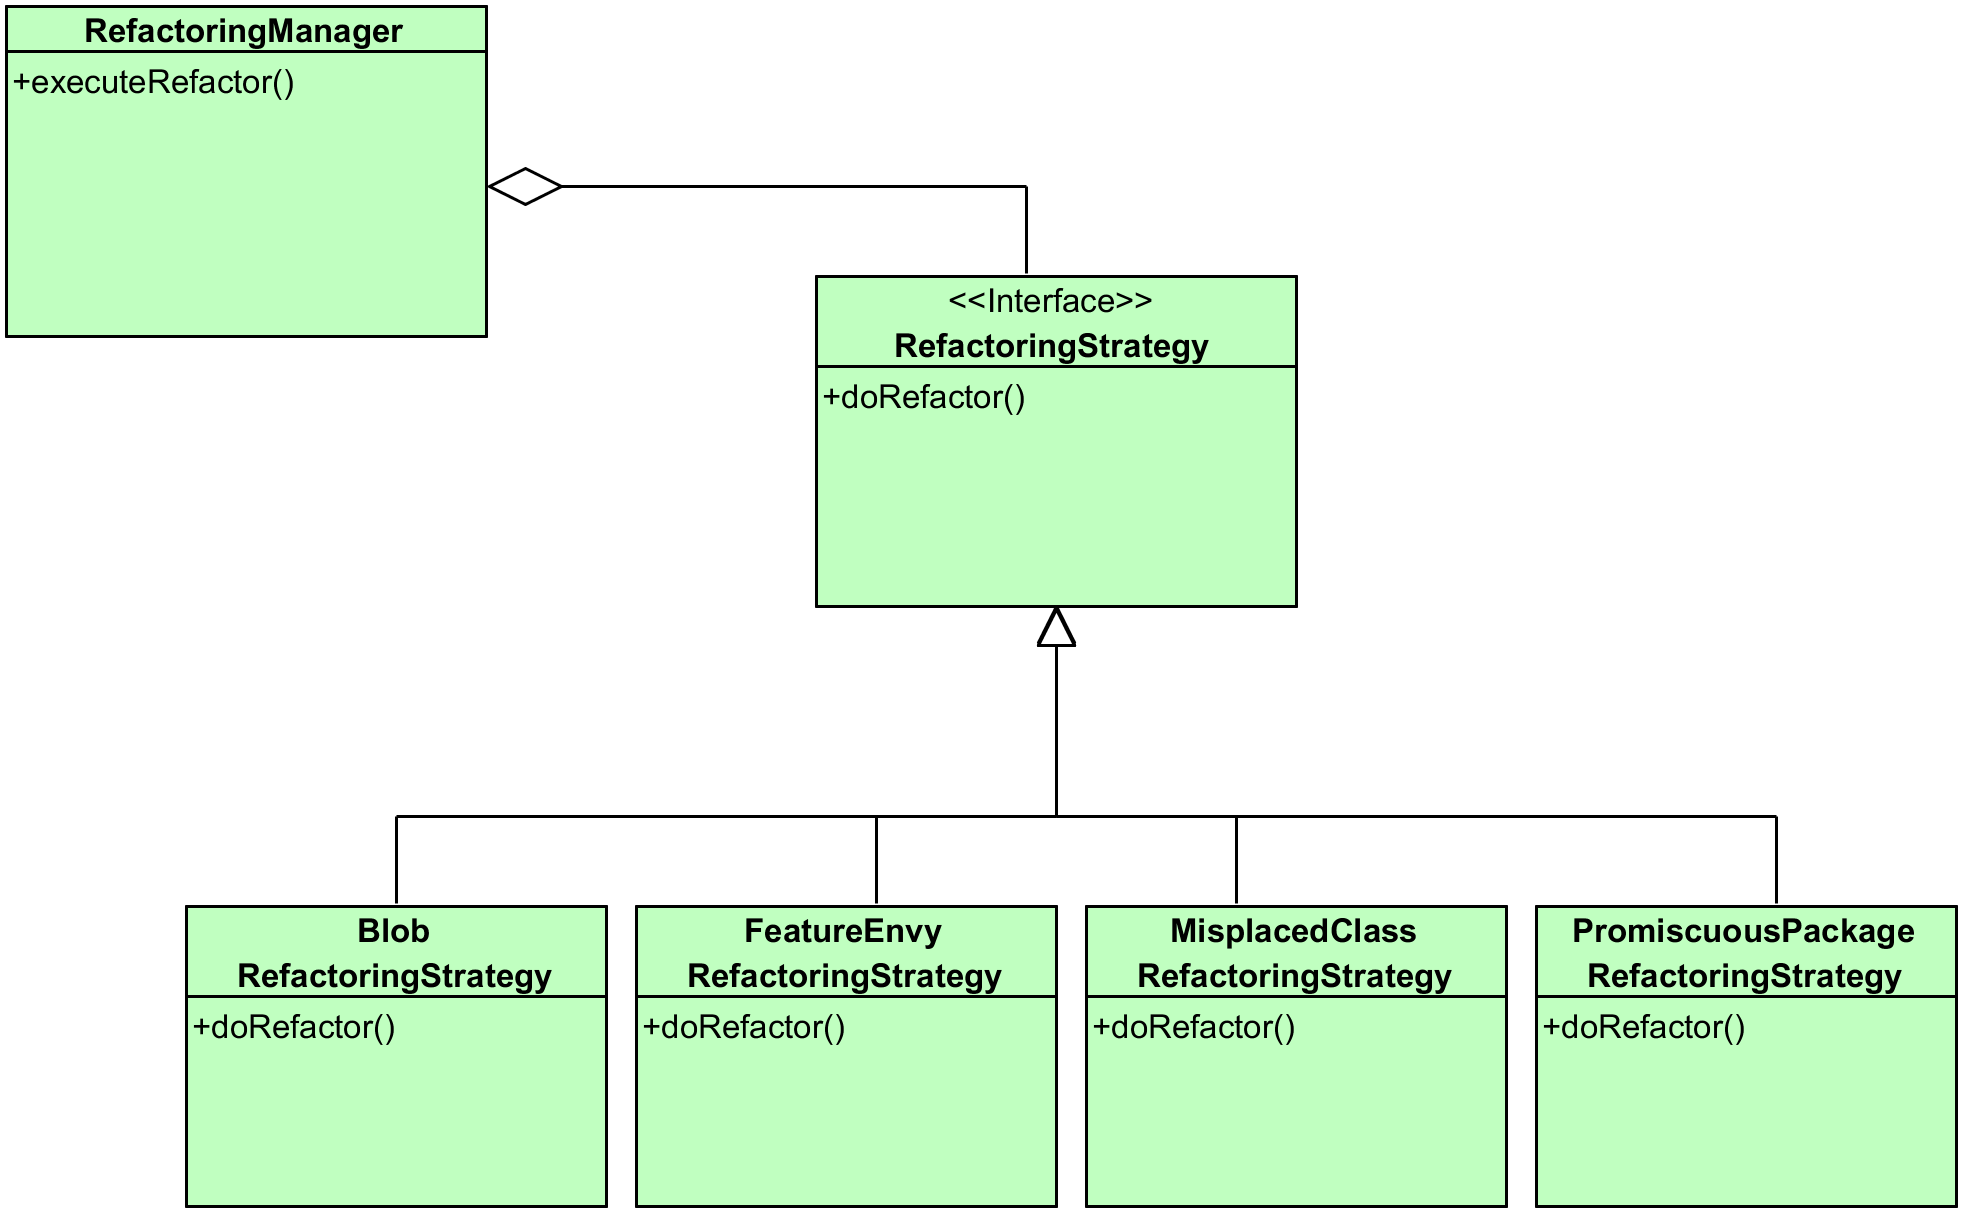
\includegraphics[width=11cm]{diagrams/RefactorStrategy}
		\end{figure}
	
			
		Per l'analisi abbiamo un'interfaccia "CodeSmellDetectionStrategy" che viene estesa dalle seguenti interfacce: ClassSmellDetectionStrategy, MethodSmellDetectionStrategy, PackageSmellDetectionStrategy.
		
		L'interfaccia ClassSmellDetectionStrategy è implementata da tre classi concrete, ossia TextBlobStrategy, StructuralMisplacedClassRule e TextualMisplacedClassStrategy.	
		
		L'interfaccia MethodSmellDetectionStrategy è implementata da due classi concrete, ossia StructuralFeatureEnvyRule e TextualFeatureEnvyRule. 
		
		L'interfaccia PackageSmellDetectionStrategy è implementata da una classe concreta, ossia TextualPromiscuousPackageStrategy.
		
		 \begin{figure}[!h]
			\centering
			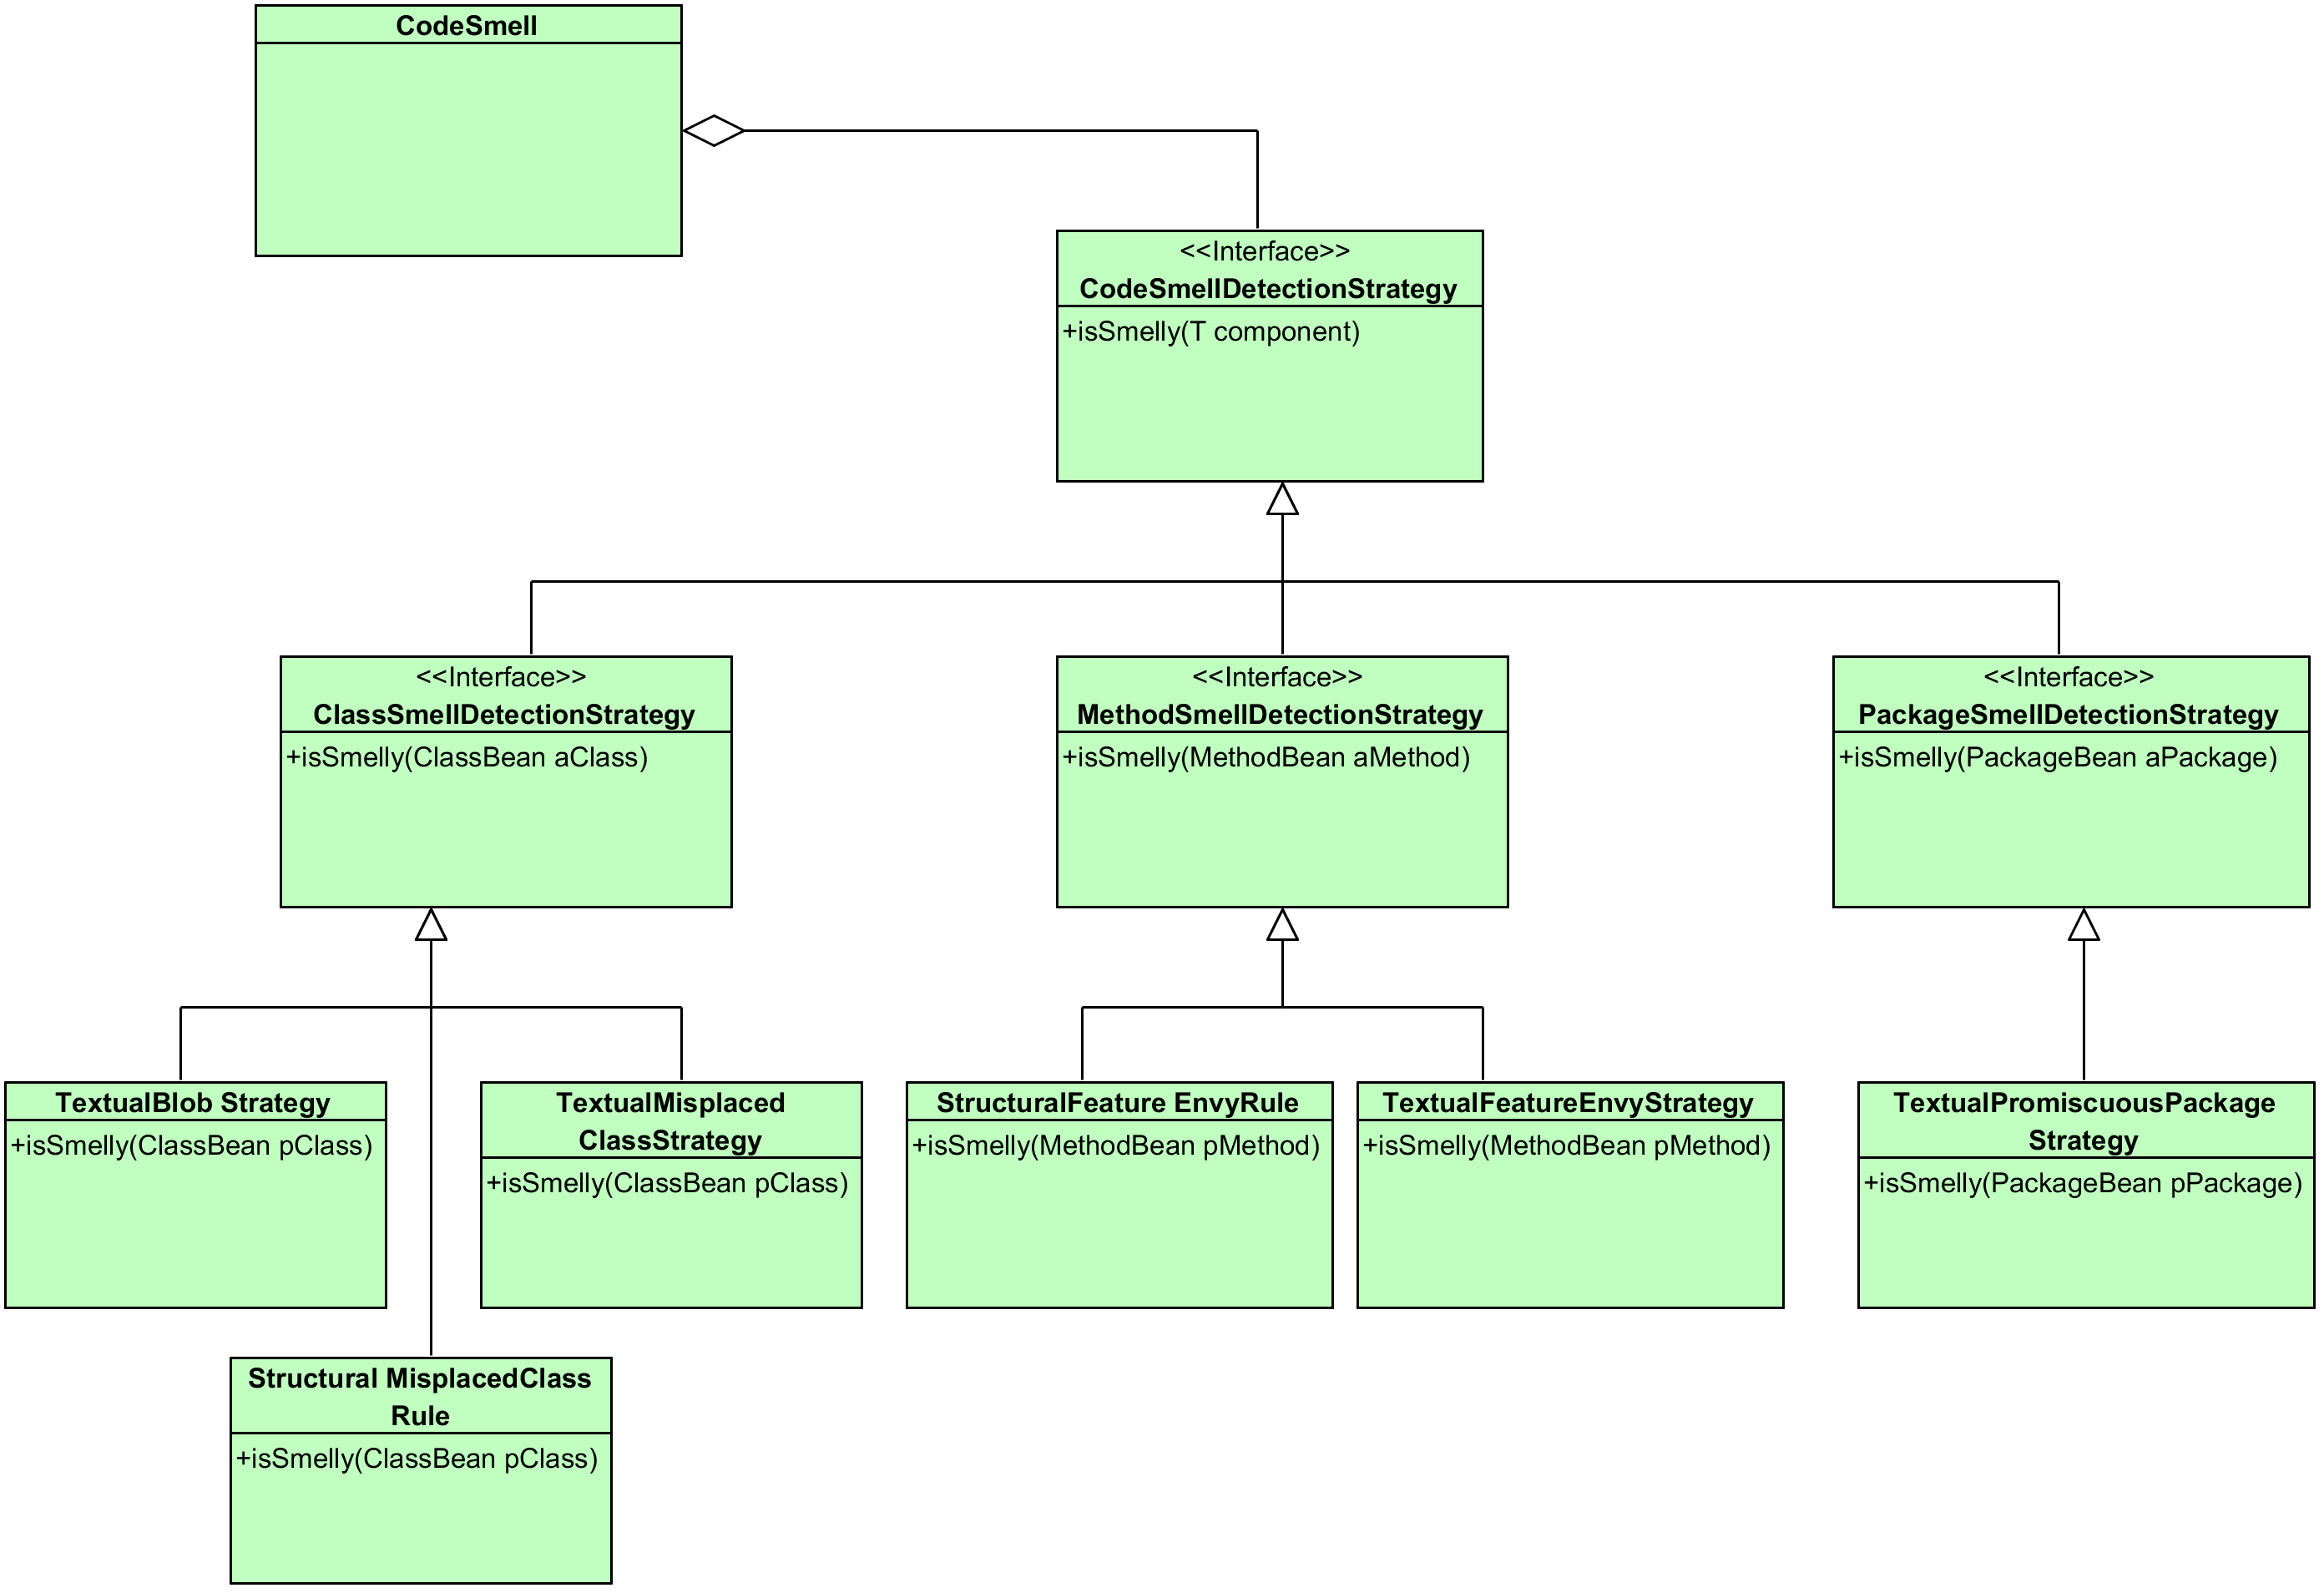
\includegraphics[width=15cm]{diagrams/AnalysisStrategy}
		\end{figure}	
	
	
		\subsection{Proxy Pattern}
	
	Si tratta di un pattern strutturale basato su oggetti che viene utilizzato per accedere
	ad un un oggetto complesso tramite un oggetto semplice.
	
	Questo pattern viene utilizzato per caricare una versione semplificata di oggetti di tipo
	InstanceVariableList, MethodList, ClassList tramite le classi proxy InstanceVariableListProxy,
	MethodListProxy, ClassListProxy.
	
	Il client può accedere a queste classi tramite interfacce "InstanceVariableBeanList",
	"MethodBeanList", "ClassBeanList".
	
	 \begin{figure}[!h]
		\centering
		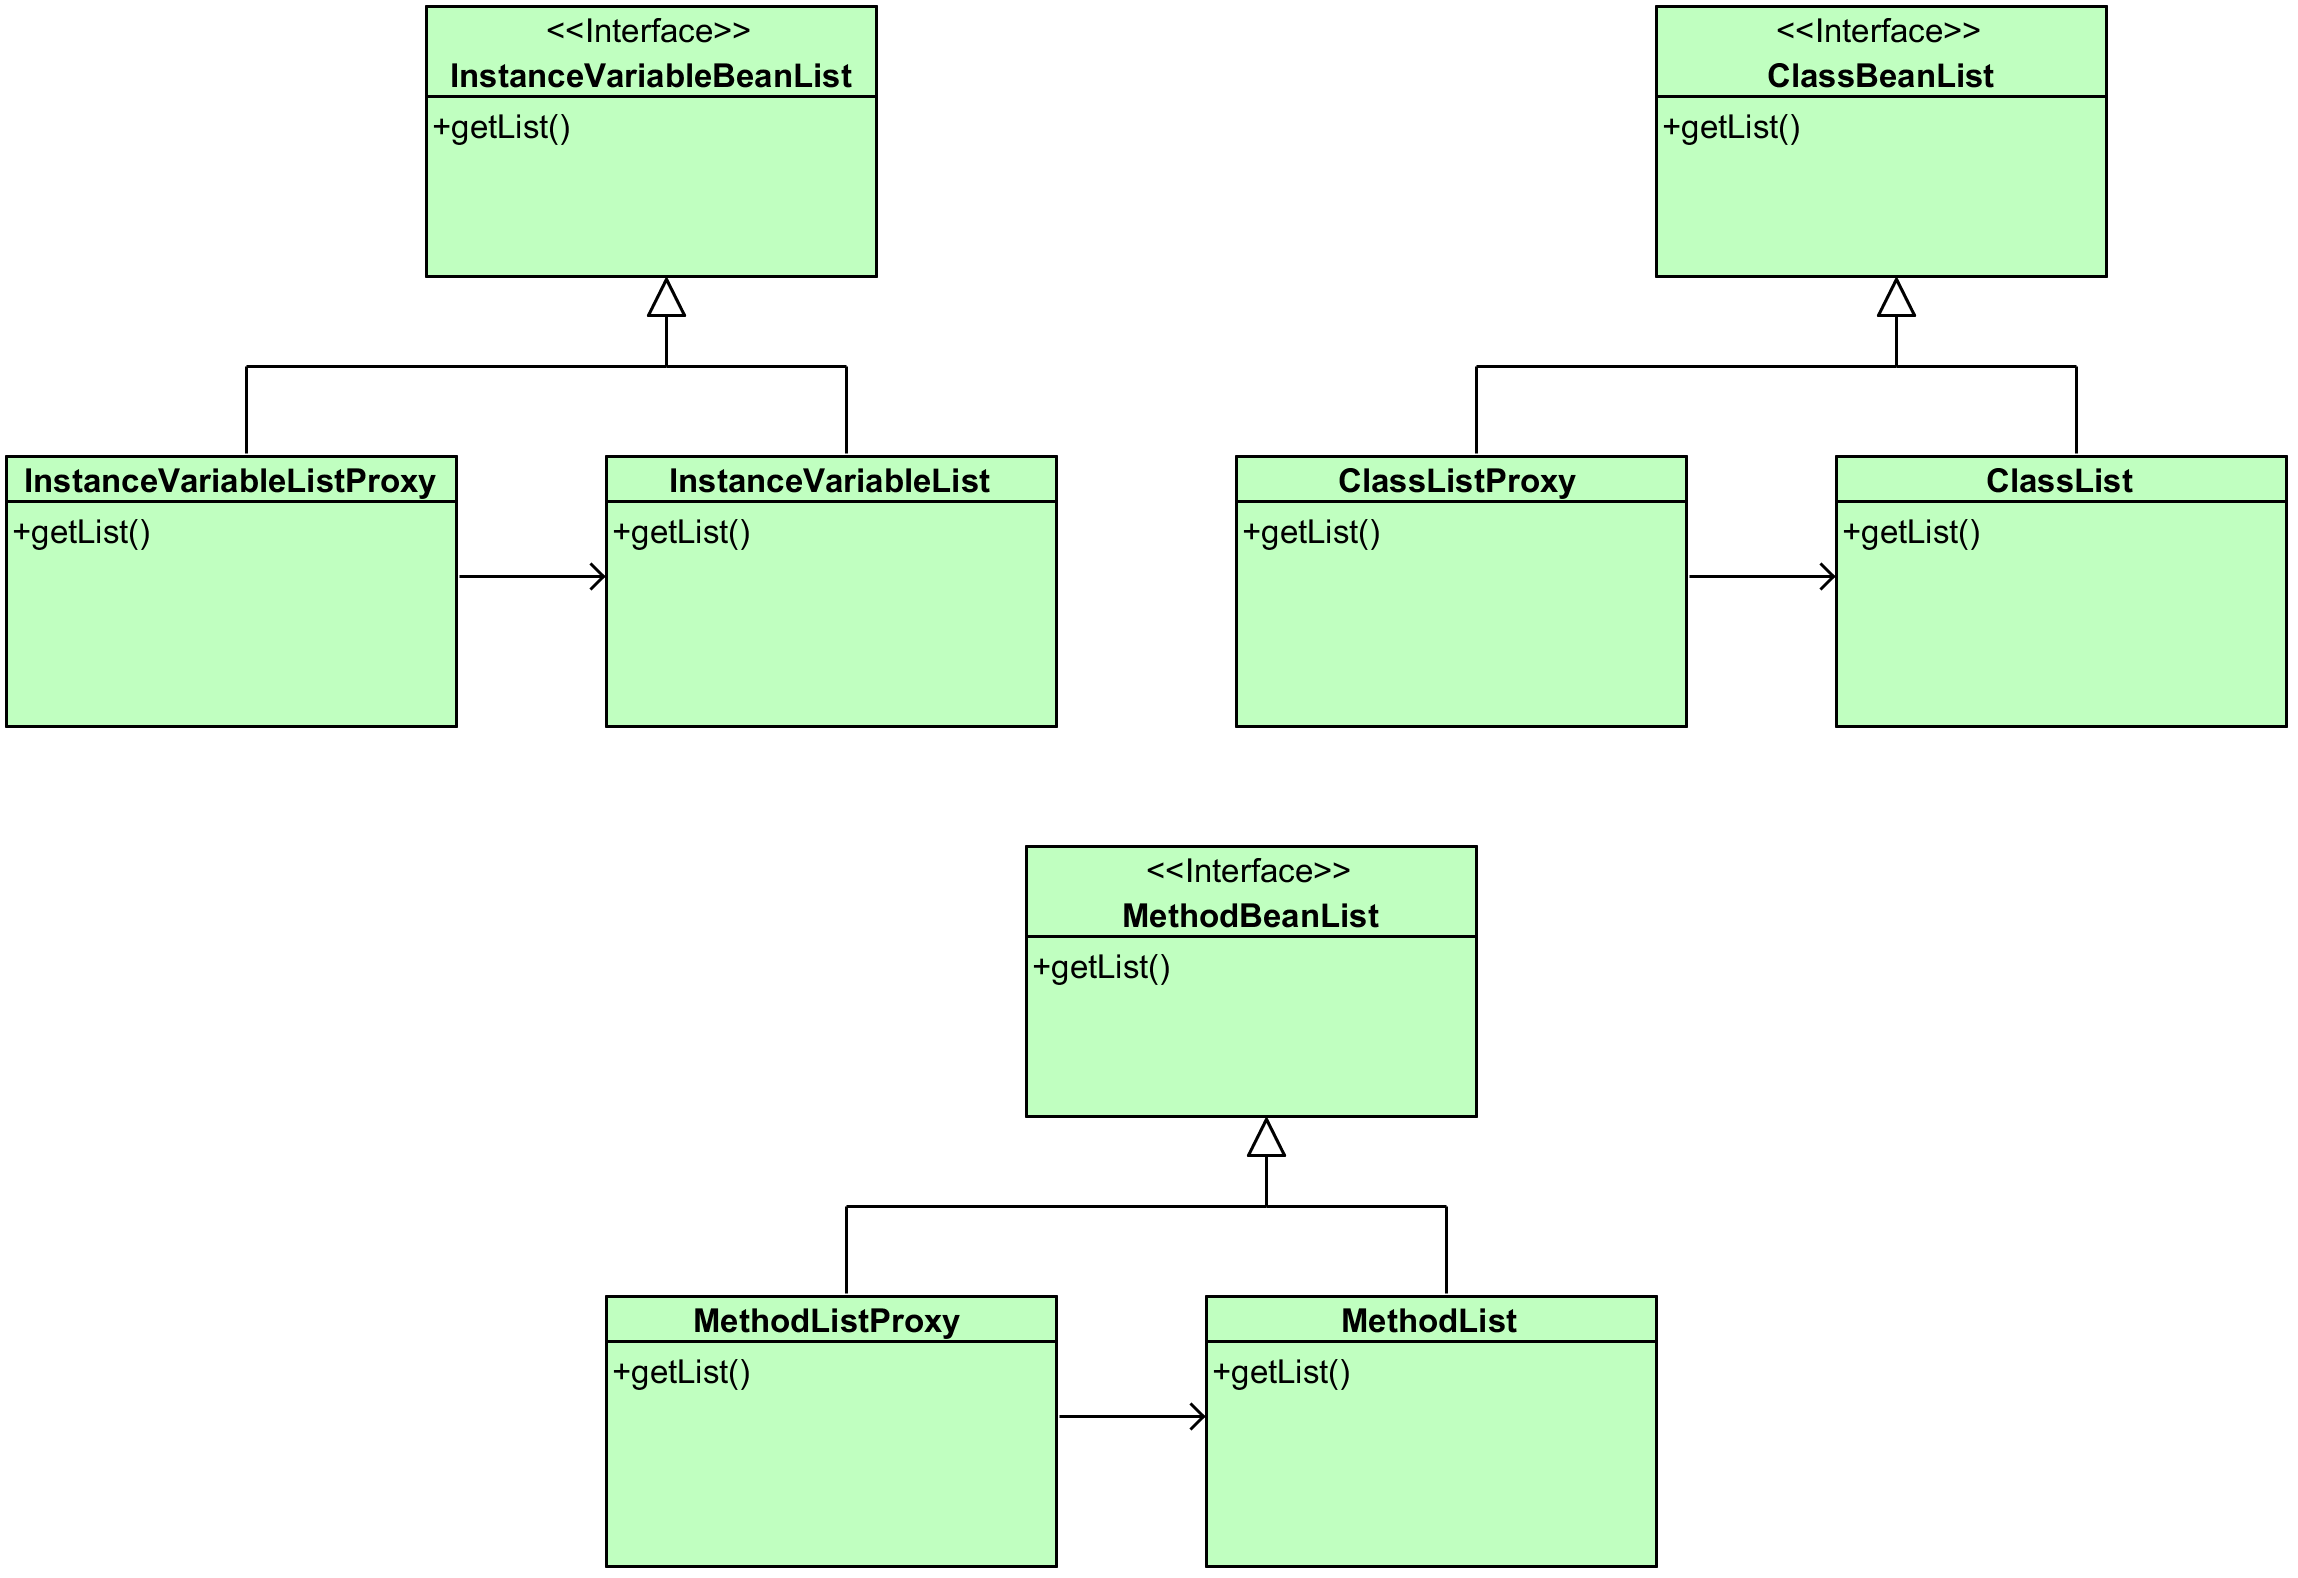
\includegraphics[width=13cm]{diagrams/ProxyPattern}
	\end{figure}	
	

	\subsection{Builder Pattern}
	
	Si tratta di un pattern creazionale basato su oggetti e viene utilizzato per creare un oggetto senza doverne conoscere i suoi dettagli implementativi.
	Questo pattern consente di utilizzare un Client che non debba essere a conoscenza dei passi necessari al fine della creazione di un oggetto ma tali passaggi
	vengono delegati ad un Director (classe che si occupa effettivamente di costruire l'oggetto) che sa cosa e come fare.
	
	Questo pattern è usato nel sistema per costruire gli oggetti di tipo ClassBean, PackageBean, MethodBean.
	\newpage
	\subsection{Repository Pattern}
	
	I repository sono classi o componenti che incapsulano la logica necessaria per accedere ai dati sorgente. Centralizzano le funzionalità comuni di accesso ai dati,
	fornendo una migliore manutenibilità e disaccoppiando l'infrastruttura o la tecnologia utilizzata per accedere ai database dal layer del modello di dominio.
	
	Questo pattern viene utilizzato per lo storage di oggetti di tipo InstanceVariableBean, MethodBean, ClassBean, PackageBean.	
	
	Per implementare questo pattern utilizziamo l'interfaccia "Repository" che viene estesa dalle
	seguenti interfacce: InstanceVariableBeanRepository, MethodBeanRepository, ClassBeanRepository, PackageBeanRepository.
	
	L'interfaccia InstanceVariableBeanRepository è implementata dalla classe InstanceVariableRepository.
	
	L'interfaccia MethodBeanRepository è implementata dalla classe MethodRepository.
	
	L'interfaccia ClassBeanRepository è implementata dalla classe ClassRepository.
	
	L'interfaccia PackageBeanRepository	è implementata dalla classe PackageRepository.
	
\begin{figure}[!h]
		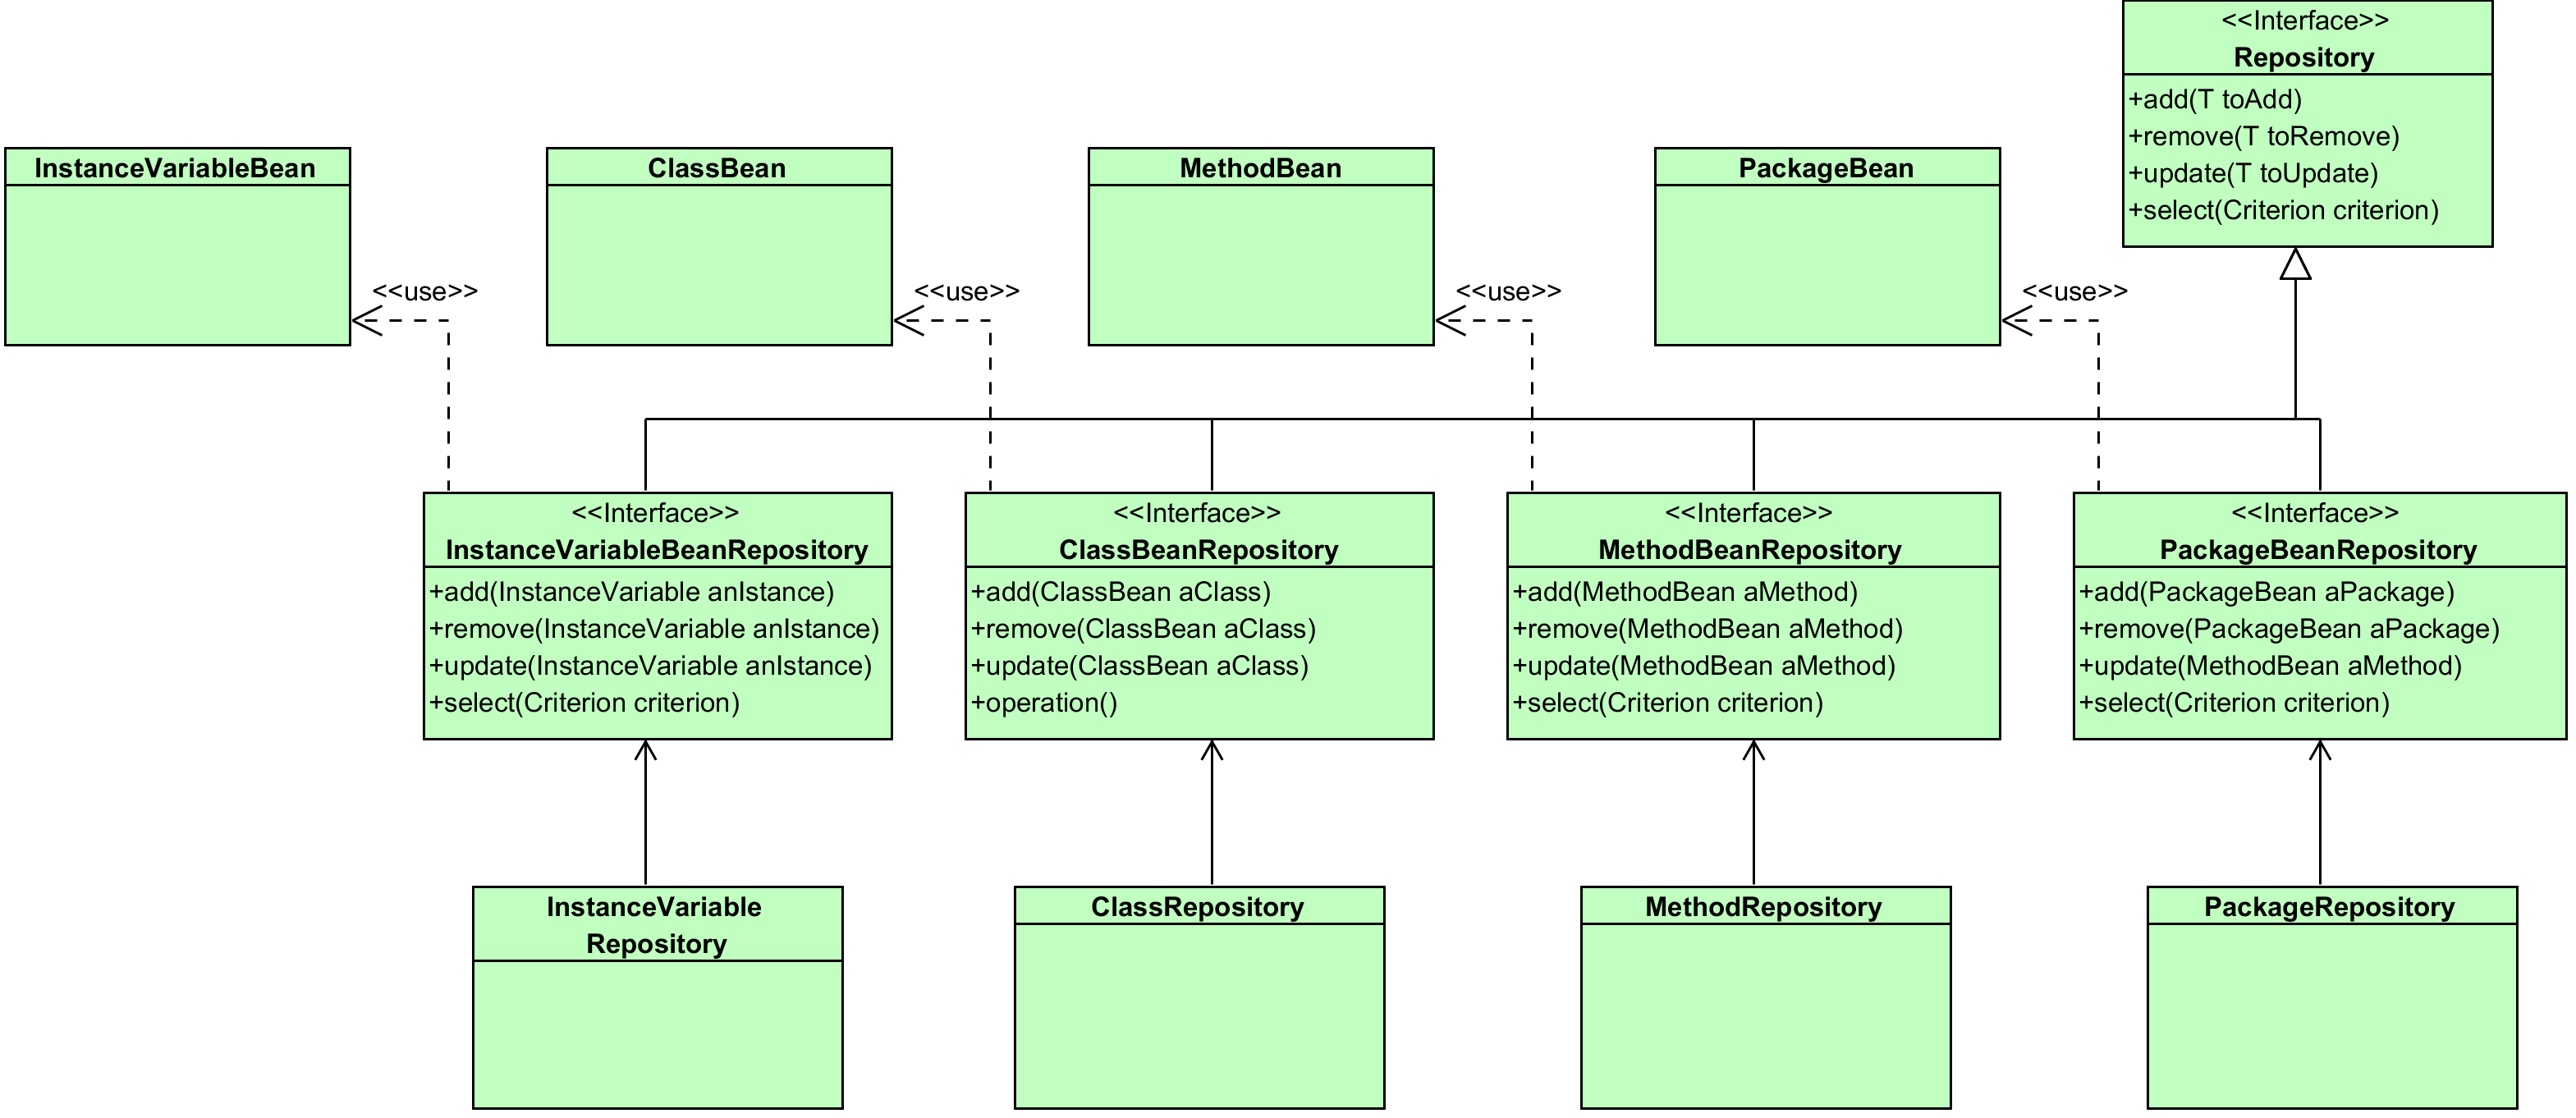
\includegraphics[width=16.5cm]{diagrams/RepositoryPattern}
	\end{figure}

\subsection{Adapter Pattern}

	L'Adapter è un pattern strutturale che può essere basato sia su classi (Class Adapter) che su oggetti (Object Adapter) e il suo scopo è convertire le interfacce di una classe in altre interfacce, attese dai client, per far sì che classi con interfacce di differenti e incompatibili possano comunque poter comunicare tra loro.
	
	Questo pattern viene utilizzato per costruire le RadarMap di ogni Bean.
	
	Per questo pattern è stata definita l'interfaccia "RadarMapUtils", che viene implementata dalla classe RadarMapUtilsAdapter.
	
	\begin{figure}[!h]
		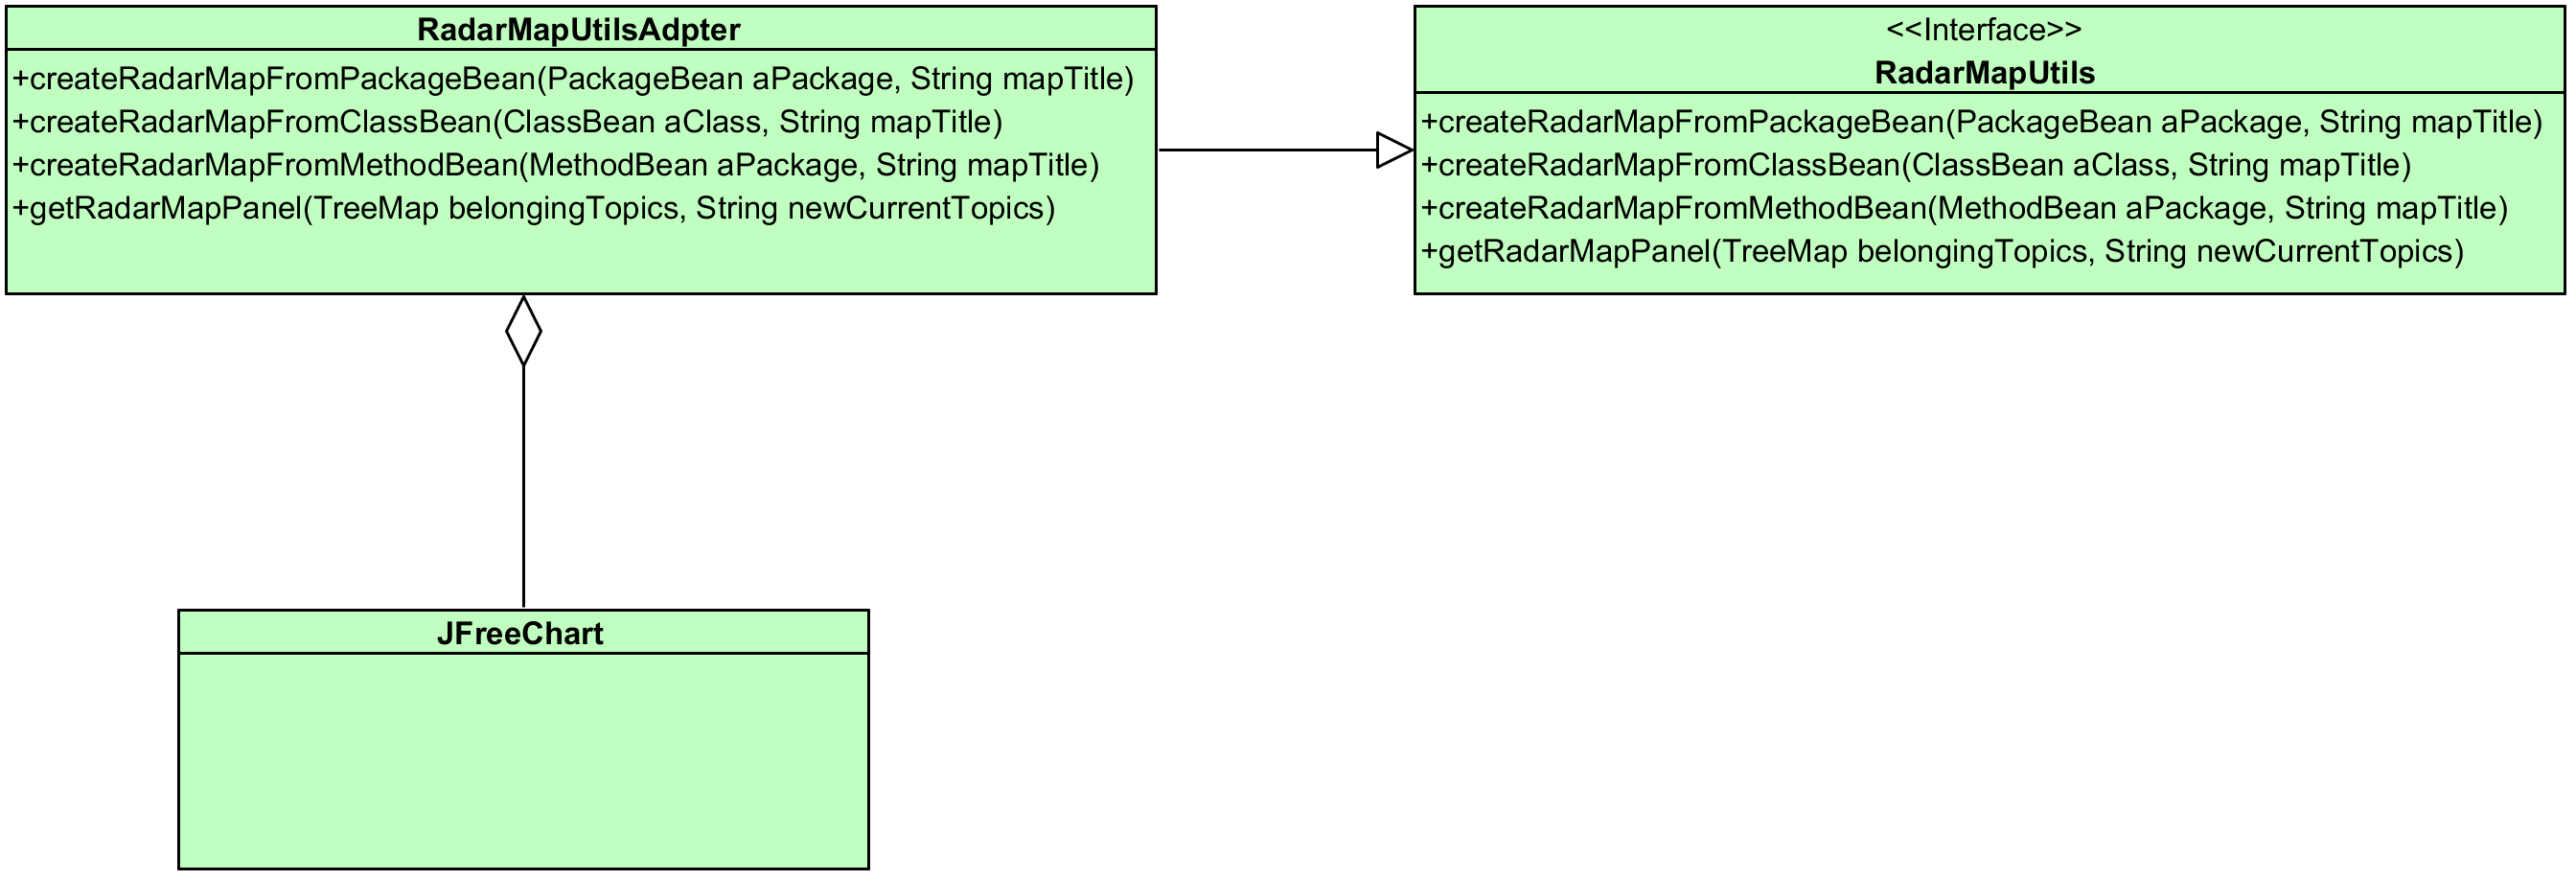
\includegraphics[width=16.5cm]{diagrams/AdapterPattern}
	\end{figure}
	

\end{document}